% Important: The shell-escape flag is required for the Minted package.
% Please compile this document with 'pdflatex -shell-escape main.tex'.
% If you are using another IDE, you may be able to specify this in the
% options or to provide an option like '% !TEX option = -shell-escape'
% in this file, depending on your builder. See the README.md for more.

% Don't put any content in here.
% Don't even include content files by using \input or \inlcude.
% Put your content into components/text.tex or include it there using \input.
% You probably want to modify the following files:
%   components/info.tex             contains the author, title etc.
%   components/settings.tex         contains the packages and settings.
%   components/commands.tex         contains helpful custom commands.
%   components/glossary.tex         contains an explanation of the used terms.
%   components/acknowledgements.tex contains the acknowledgements.
%   components/quote.tex            contains a quote.
%   components/abstract.tex         contains the abstract of the document.
%   components/text.tex             includes the actual content of the document.
%   components/outline.tex          contains the outline.
%   components/preface.tex          contains the preface.
%   chapters/                       contains the main text.
%   bibliography/literature.bib     contains the BibTeX entries.
%   images/                         contains all your content-related images.
%
% You probably don't need to change anything in the following files:
%   components/cover.tex            formats the front cover of the document.
%   components/titlepage.tex        formats the title page of the document.
%   components/disclaimer.tex       formats the disclaimer page.
%   styles/                         contains style elements (e.g. logos).
%   main.tex                        contains the top-level code structure.
%   README.md                       contains information about this template.

\documentclass[11pt,
              a4paper,
              article,
              index=totoc,
              headsepline,
              footsepline,
              BCOR=12mm,
              DIV=13]{scrbook}
\setcounter{secnumdepth}{3}
\usepackage{amsthm}
\usepackage[ruled,vlined]{algorithm2e}
\usepackage{tikz}
\usepackage{wrapfig}
\usetikzlibrary{shapes,arrows,positioning}
\setlength{\parindent}{0pt}
\usepackage{xcolor}
\usepackage{caption}
\usepackage{subcaption}
\usepackage{adjustbox}
% KOMA scrbook options:
%  index=totoc: include an entry for the index in the table of contents.
%  headsepline: use horizontal line under heading.
%  footsepline: use horizontal line above footer.
%  BCOR: binding correction (e.g.: BCOR=12mm)
%  DIV: Number of sheet sections (used for layout) (e.g.: DIV=13)


%  This code base is currently hosted at: 
%  https://github.com/waltsims/TUM_Thesis_Template_CSE
\usepackage[backend=biber, sorting=none]{biblatex}
\addbibresource{bibliography/literature.bib}
% !TEX root = ../main.tex
% Set here the title, authors and other stuff to be used for the cover
% This file is used by MAIN.TEX

% set title, authors and stuff for the cover
\def\university{Technische Universit{\"a}t M{\"u}nchen}
\def\universityLogo{styles/tum_logo}
\def\program{Robotics, Cognition, Intelligence (M.Sc.)}
\def\programLogo{styles/cse_logo}
\def\doctype{Master's Thesis}

\def\title{A Noval Approach For Inference Time Search On Continuous Action Space in Deterministic Environments}
\def\author{Hendrik Elvers}
\def\supervisor{Prof. Dr.-Ing. habil. Alois Knoll}
\def\advisor{Dr. rer. nat. Zhenshan Bing}
\def\date{April 15th, 2023}

\def\keywords{{RL}, {IL}, {POMDP}}

% The following are used for the PDF metadata, by default the same as above.
\def\metaTitle{\title}
\def\metaAuthor{\author}
\def\metaSubject{\doctype\ -\ \university}
\def\metaKeywords{\keywords}

% text to appear in the footer
\def\footertext{}


% !TEX root = ../main.tex
% Included by MAIN.TEX

%--------------------------------------------------
% Fonts and page setup
%--------------------------------------------------

% Default font
\usepackage{palatino}

% Enable special PostScript fonts (optional)
% \usepackage{pifont}

% Manipulate the footer
\usepackage{scrlayer-scrpage}
\usepackage{scrhack}
\pagestyle{scrheadings}
\ifoot[\footertext]{\footertext} % \footertext set in INFO.TEX

% Set the font for the section headings
\renewcommand{\sectfont}{\normalfont \bfseries}

% Conditional commands in LaTeX documents, used for the \clearemptydoublepage.
\usepackage{ifthen}

% Typeset text in multiple columns (optional)
% \usepackage{multicol}

% Rotation tools, including rotated full-page floats (optional)
\usepackage{rotating}


%--------------------------------------------------
% Document structure
%--------------------------------------------------

% Pro­duce hy­per­text links in the doc­u­ment (recommended)
\usepackage{hyperref}

% Create glossaries and lists of acronyms
% depending on how many packages were shipped with your TeX distribution,
% you might need to install xindy. On Linux: sudo apt install xindy
\usepackage[toc, xindy]{glossaries}

% Standard LaTeX package for creating indexes
\usepackage{makeidx}


%--------------------------------------------------
% Bibliography
%--------------------------------------------------

% Set the bibliography style (default: plain)
\bibliographystyle{plain}

% Special biblography package (nice to have)
% \usepackage{natbib}


%--------------------------------------------------
% Graphics and floats
%--------------------------------------------------

% Enhanced support for graphics (recommended)
\usepackage{graphicx}
% Path to the figures directory (default: {figures/})
% Multiple entries are allowed, e.g. {{figures1/}{figures2/}}.
\graphicspath{{figures/}}

% Improved interface for floating objects (optional)
\usepackage{float}

% To use the subfigures (optional)
\usepackage{subcaption}


%--------------------------------------------------
% Mathematics
%--------------------------------------------------

% AMS mathematical facilities for LaTeX (recommended)
\usepackage{amsmath}

% TeX fonts from the American Mathematical Society (recommended)
\usepackage{amsfonts}

% Some extra math symbols (optional)
% \usepackage{amssymb}

% Extended maths fonts for LaTeX (optional)
% \usepackage{yhmath}

% Provide math delimiters whose size can be computed automatically (optional)
% \usepackage{commath}


%--------------------------------------------------
% Source code and algorithms
%--------------------------------------------------

% Source code typesetting
% \usepackage{listings} % (optional - alternative)
\usepackage[newfloat]{minted} % (recommended)
% Set global Minted options
\setminted{linenos, autogobble, frame=lines, framesep=2mm}
% Inline C++ (optional)
\newcommand{\incpp}[1]{\mintinline{c++}{#1}}
\newenvironment{code}{\captionsetup{type=listing}}{}
\SetupFloatingEnvironment{listing}{name=Source Code}

% Typeset algorithms - pseudocode (optional)
% \usepackage{algorithmicx}
% \usepackage{algpseudocode}
% Normal arrow comments
% \algrenewcommand{\algorithmiccomment}[1]{\hfill$\rightarrow$ #1}


%--------------------------------------------------
% Tables
%--------------------------------------------------

% Tables (optional)
\usepackage{tabu}

% Add color to LaTeX tables (optional)
% \usepackage{colortbl}

% Create tabular cells spanning multiple rows (optional)
% \usepackage{multirow}


%--------------------------------------------------
% Color
%--------------------------------------------------

% Use colors
\usepackage[dvipsnames]{xcolor}

% You may find all the pre-defined colors in
% https://en.wikibooks.org/wiki/LaTeX/Colors#Predefined_colors

% Custom colors
\definecolor{Pantone300C}{HTML}{0065BD} % TUM primary blue
\definecolor{Pantone301}{HTML}{005293}  % TUM secondary light blue
\definecolor{Pantone540}{HTML}{003359}  % TUM secondary dark blue
\definecolor{DarkGray}{HTML}{333333}    % TUM secondary dark gray
\definecolor{MediumGray}{HTML}{808080}  % TUM secondary medium gray
\definecolor{LightGray}{HTML}{CCCCC6}   % TUM secondary light gray
\definecolor{Pantone7527}{HTML}{DAD7CB} % TUM accent gray
\definecolor{Pantone158}{HTML}{E37222}  % TUM accent orange
\definecolor{Pantone383}{HTML}{A2AD00}  % TUM accent green
\definecolor{Pantone283}{HTML}{98C6EA}  % TUM accent very light blue
\definecolor{Pantone542}{HTML}{64A0C8}  % TUM accent light blue

% Color for the hyperlinks (e.g. table of contents)
\def\colorLinks{Pantone300C}
% Color for the web links
\def\colorUrl{Pantone542}
% Color for the citations
\def\colorCitations{Pantone158}

%--------------------------------------------------
% PDF output
%--------------------------------------------------

% Adjust the color of the links
\hypersetup{
  linkcolor=\colorLinks,%
  urlcolor=\colorUrl,%
  citecolor=\colorCitations
}

% Disable the coloring of the links when printing.
% Requires a compatible PDF reader.
\usepackage[ocgcolorlinks]{ocgx2}[2017/03/30]

% PDF Metadata
\hypersetup{
  pdftitle={\metaTitle},%
  pdfauthor={\metaAuthor},%
  pdfkeywords={\metaKeywords},%
  pdfsubject={\metaSubject}
}

% Create XMP Metadata (uses the values from hyperref)
\usepackage{hyperxmp}

% Make thumbnails (optional)
% \usepackage{thumbpdf}


%--------------------------------------------------
% Other settings
%--------------------------------------------------

% Define commands that appear not to eat spaces (optional)
\usepackage{xspace}


% !TEX root = ../main.tex
% Included by MAIN.TEX
% Please include your own cool commands here.
% Be only sure to comment it sufficiently so others can use it.

%-------------------------------------------------------------
%                      Own Commands
%-------------------------------------------------------------


%-------------------------------------------------------------
% math stuff -------------------------------------------------

% nice R, N, C
\newcommand{\nat}{\mathbb{N}}
\newcommand{\real}{\mathbb{R}}
\newcommand{\compl}{\mathbb{C}}

% un demi
\newcommand{\half}{\frac{1}{2}}

% parantheses
\newcommand{\parenth}[1]{ \left(#1 \right) }
\newcommand{\bracket}[1]{ \left[#1 \right] }
\newcommand{\accolade}[1]{ \left\{ #1 \right\} }
%\newcommand{\angle}[1]{ \left\langle  #1 \right\rangle }

% partial derivative: %#1 function, #2 which variable
% simple / single line version
\newcommand{\pardevS}[2]{ \delta_{#1} f(#2) }

% fraction version
\newcommand{\pardevF}[2]{ \frac{\partial #1}{\partial #2} }

% render vectors: 3 and 4 dimensional
\newcommand{\veciii}[3]{\left[ \begin{array}[h]{c} #1 \\ #2 \\ #3	\end{array} \right]}
\newcommand{\veciv}[4]{\left[ \begin{array}[h]{c} #1 \\ #2 \\ #3 \\ #4	\end{array} \right]}

% render matrices: 3  dimensional (arguments in row first order)
\newcommand{\matiii}[9]{\left[ \begin{array}[h]{ccc} #1 & #2 & #3 \\ #4 & #5 & #6 \\ #7 & #8 & #9	\end{array} \right]}

%-------------------------------------------------------------
% some abreviations ------------------------------------------
\newcommand{\Reg}{$^{\textregistered}$}
\newcommand{\reg}{$^{\textregistered}$ }
\newcommand{\Tm}{\texttrademark}
\newcommand{\tm}{\texttrademark~}
\newcommand {\bsl} {$\backslash$}

%-------------------------------------------------------------
% formating --------------------------------------------------

% Theorem & Co environments and counters
\newtheorem{theorem}{Theorem}[chapter]
\newtheorem{lemma}[theorem]{Lemma}
\newtheorem{corollary}[theorem]{Corollary}
\newtheorem{remark}[theorem]{Remark}
\newtheorem{definition}[theorem]{Definition}
\newtheorem{equat}[theorem]{Equation}
\newtheorem{example}[theorem]{Example}
%\newtheorem{algorithm}[theorem]{Algorithm}

% inserting figures
\newcommand{\insertfigure}[4]{ % Filename, Caption, Label, Width percent of textwidth
	\begin{figure}[htbp]
		\begin{center}
			\includegraphics[width=#4\textwidth]{#1}
		\end{center}
		\vspace{-0.4cm}
		\caption{#2}
		\label{#3}
	\end{figure}
}

% referecing figures

\newcommand{\refFigure}[1]{ %label
	Figure~\ref{#1}
}
\newcommand{\refChapter}[1]{ %label
	Chapter~\ref{#1}
}

\newcommand{\refSection}[1]{ %label
	Section~\ref{#1}
}

\newcommand{\refParagraph}[1]{ %label
	Paragraph~\ref{#1}
}

\newcommand{\refEquation}[1]{ %label
	Equation~\ref{#1}
}

\newcommand{\refTable}[1]{ %label
	Table~\ref{#1}
}

\newcommand{\rigidTransform}[2]
{
	${}^{#2}\!\mathbf{H}_{#1}$
}

% comment that appears on the border - very practical !!!
\newcommand{\comment}[1]{\marginpar{\raggedright \noindent \footnotesize {\textsl{#1}} }}

% page clearing
\newcommand{\clearemptydoublepage}{%
  \ifthenelse{\boolean{@twoside}}{\newpage{\pagestyle{empty}\cleardoublepage}}%
  {\clearpage}}

%-------------------------------------------------------------
%-------------------------------------------------------------

\newcommand{\etAl}{\emph{et al.}\mbox{ }}


% !TEX root = ../main.tex
\newglossaryentry{computer}
{
  name=computer,
  description={is a programmable machine that receives input,
               stores and manipulates data, and provides
               output in a useful format}
}

\newglossaryentry{poc}
{
  name={proof of concept},
  description={}
  }
\newglossaryentry{ui}
{
  name={user interface},
  description={}
  }
\newglossaryentry{ai}
{
  name={arithmetic intensity},
  description={a measure of floating-point operations (FLOPs)
              \hyphenation{per-formed} performed by a \hyphenation{gi-ven} given code or code section relative
              to the amount of memory accesses (Bytes) that are required
               to support those operations\cite{AI}}
  }

\newglossaryentry{speed-up}
{
  name={speed-up},
  description={the factor of temporal acceleration a program
  exhibits when additional computational resources are dedicated to it's execution.}
}

\newglossaryentry{directive pragmas}
{
  name={directive pragma},
  description={a computer programming language construct that specifies how a compiler
  should process input data} % sourced from wikipedia
}


\newglossaryentry{rc}{%SOURCE: wikipedia
name={race condition},
description={A race condition or race hazard is the behaviour of an electronic,
 software, or other system where the output is dependent on the sequence or
 timing of other uncontrollable events. It becomes a bug when events do not
 happen in the order the programmer intended. The term originates with the idea
 of two signals racing each other to influence the output first.}
}
\newglossaryentry{dd}{
name={data dependencies},
description={}
}
\newglossaryentry{sisd}{
name={single instruction single data},
description={}
}
\newglossaryentry{simt}{
name={single instruction multiple threads},
description={}
}

\newglossaryentry{simd}{
name={single instruction multiple data},
description={}
}
\newglossaryentry{gp}{%SOURCE: wikipedia
name={Gaussian Plane},
description={The two dimensional plane of complex numbers.}
}
\newglossaryentry{CURAND}{
name={CURAND},
description={
The CURAND library provides facilities that focus on the simple and efficient
generation of high-quality pseudorandom and quasirandom numbers.\cite{cuRAND}
}
}

\newacronym[longplural={partial differential equations}]{PDE}{PDE}{partial differential equations}
\newacronym{mpi}{MPI}{Message Passing Interface}

\newacronym[longplural={Random Walks on Spheres}]{RWoS}{RWoS}{Random Walk on Spheres}

\newacronym[longplural={graphical processing units}]{GPU}{GPU}{graphical processing unit}

\newacronym[longplural={central processing units}]{CPU}{CPU}{central processing unit}
\newacronym{hpc}{HPC}{high performance computing}

\newacronym[longplural={arithmetic logic units}]{ALU}{ALU}{arithmetic logic unit}

\newacronym[longplural={streaming multi-processors}]{SM}{SM}{streaming multi-processor}

\newacronym[longplural={boundary value problems}]{BVP}{BVP}{boundary value problem}
\newacronym[longplural={general purpose graphical processing units}]{GPGPU}{GPGPU}{general purpose graphical processing units}
\newacronym{CUDA}{CUDA}{compute unified device architecture}
\newacronym{RAM}{RAM}{random access memory}
\newacronym{SRAM}{SRAM}{static random access memory}
\newacronym{DRAM}{DRAM}{dynamic random access memory}
\newacronym{I/O}{I/O}{input/output}
\newacronym{PTX}{PTX}{Parallel Thread eXecution}
\newacronym{jit}{JIT}{just in time}


\makeglossaries

\begin{document}

 \frontmatter

 % !TEX root = ../main.tex
% The front cover.
% Included by MAIN.TEX

%--------------------------------------------------
% The Front Cover
%--------------------------------------------------

% correct BCOR - undo at the end !!!
\def\bcorcor{0.15cm}
\addtolength{\hoffset}{\bcorcor}

\thispagestyle{empty}

\vspace{4cm}
\begin{center}
	\includegraphics[width=4cm]{\universityLogo}\\
	\vspace{5mm}
	\huge \university \\
	\vspace{0.5cm}

	\Large \department \\
	\vspace{0.5cm}

	\Large \doctype\\
	\vspace{0.5cm}
\end{center}

\vspace{20mm}
\begin{center}
	\vspace{20mm}
	{\huge \textbf \title}\\
	\vspace{15mm}
	{\LARGE  \author}\\
	\vspace{\fill}
\end{center}


 \clearemptydoublepage

 % !TEX root = ../main.tex
% The titlepage.
% Included by MAIN.TEX


%--------------------------------------------------
% The title page
%--------------------------------------------------

% correct BCOR - undo at the end !!!
\def\bcorcor{0.15cm}
\addtolength{\hoffset}{\bcorcor}

\thispagestyle{empty}

\vspace{4cm}
\begin{center}
    \includegraphics[width=4cm]{\universityLogo}\\
    \vspace{5mm}
    \huge \program \\
    \vspace{0.5cm}
    \large \university
\end{center}

\vspace{10mm}
\begin{center}
    {\Large \doctype}\\
    \vspace{10mm}
    {\LARGE \title}\\
    \vspace{10mm}

    \begin{tabular}{ll}
      \Large Author:                        & \Large \author \\[2mm]
      \Large Supervisor:                    & \Large \supervisor \\[2mm]
      \Large Advisor:                       & \Large \advisor \\[2mm]
      \Large Submission Date:               & \Large \date
    \end{tabular}

    \vspace{\fill}
    \includegraphics[width=4cm]{\programLogo}
\end{center}

% undo BCOR correction
\addtolength{\hoffset}{\bcorcor}


 % !TEX root = ../main.tex
\clearemptydoublepage

\thispagestyle{empty}
\vspace*{0.8\textheight}
\noindent
I confirm that this master's thesis is my own work and I have documented all sources and material used.


\vspace{15mm}
\noindent
\date \hspace{5cm} \author
\newpage


 % !TEX root = ../main.tex
% The abstract.
% Included by MAIN.TEX
\clearemptydoublepage
\phantomsection
\addcontentsline{toc}{chapter}{Abstract}

\vspace*{2cm}
\begin{center}
{\Large \textbf{Abstract}}
\end{center}
\vspace{1cm}

\chapter*{Abstract}
\label{chapter:Abstract}

\ac{rl} has shown remarkable progress in recent years, but still faces challenges in solving tasks with high-dimensional 
continuous state and action spaces, and sparse rewards. This thesis proposes a new \ac{rl} paradigm called \ac{avc}, which uses search at 
inference time and leverages expert demonstrations to overcome these challenges. \ac{avc} is a general-purpose algorithm applicable to both deterministic 
\ac{mdp}s and deterministic \ac{pomdp}s, and is the first algorithm to use inference-time search on continuous 
action spaces without a given model of the environment.\\

In this thesis, we investigate the effectiveness of \ac{avc} in solving tasks with sparse rewards and limited observations. We test \ac{avc} on 
a setup where a single observation per trajectory is provided along with expert demonstrations, as well as on an \ac{mdp} setting with observations 
after each step. We compare \ac{avc}'s performance to state-of-the-art \ac{rl} algorithms and a state-of-the-art imitation 
learning algorithm. \\

Our experimental results show that \ac{avc} outperforms the selected baselines in both the single observation \ac{pomdp}s and \ac{mdp}s, achieving superior 
performance while maintaining high sample efficiency. We also propose several avenues for future research, such as incorporating stochastic 
observations, modelling uncertainty estimates, and incorporating curiosity-driven exploration.\\

Overall, the results demonstrate the efficacy of the \ac{avc} paradigm in leveraging expert knowledge and search to achieve swift learning and 
increased stability in challenging \ac{rl} tasks.

 \tableofcontents

 \mainmatter

 % !TEX root = ../main.tex
% Included by MAIN.TEX
% Put your content in here or include it by using \input (\include won't work)

\addtolength{\evensidemargin}{-12mm}


% !TEX root = ../main.tex
\chapter{Introduction}
\label{chapter:Introduction}
Deep reinfocement learning made promising advances in recent years. Notably, DeepMinds MuZero \cite{MUZero} can solve challenging problems leveraging deep neural networks as function approximators and 
Monte Carlo Tree Search (MCTS) to plan actions ahead. Another field that made leaps forward recently is generative AI. As examples, Midjourney \cite{midjourney} 
can produce live like pictures from natural 
language description and "ChatGPT" is able to meaningfully provide assistance from natural language inputs. \\
We identify two important paradigms from these examples: search and pretraining. In this thesis, we develop the "Active Critic" (AC) algorithm, which aims to effectively use 
expert demonstrations and conducts a search over candidate trajectories during inference time, while still beeing real time capable.\\
Search is currently not widely used in robotik, as MCTS can not be used, because the number of branches per node is infinite making enumeration impossible. While there are recent approaches 
using search on continuous action spaces \cite{Manna2022} \cite{Lee_Jeon_Kim_Kim_2020}, they require a differentiable model of the system dynamics, which is difficult to provide in real world scenarios. 
Also currenlty there are no vast datasets for robot trajectories public, so data availablitliy is limited.\\ 
In this thesis we develop a new reinforcement learning 
paradigm called "Active Critic" (AC), that learns to model only relevant aspects of the world dynamics and does search in inference time to find good solutions, with a key aspect 
of making efficient use of expert knowledge. To the authors knowledge, AC is the only algorithm that uses inference time search on continuous action space with no given model of the environment.\\

To test our algorithm, we initially choose a setup, where a single observation per trajectory is provided together with a sparse reward signal, 
indicating if the trajectory solved the environment. We also provide expert demonstrations for guidance. \\

We find this to be an interesting setting. While a single observation is not a typical assumption in current reinfocement learning approaches, it is plausible that robots in the real world 
will not have the time to do complex computation on the input signal after each time step. Moreover we think sparse rewards are a practival constraint. 
They are typically easy to define even in real world applications or sparse reward from human feedback could be used. It is well 
discussed that reward shaping is tedious and can lead to sub optimal perforance. As an example for our setup, imagine an automated production line, where a robot conducts a 
fast correction step, like cutting away bad parts of food, with high speed, based on an image of the object. A human could easily provide the feedback of wether 
the object is in the intendet state after the operation. It would be vastly more effort to provide a reward signal for every step along the trajectory and it is 
not trivial to do so in a way that is helpful for the learning algorithm. As the time to perform the trajectory could be very short, realsitically only a sparse set of images per trajectory could be 
processed. In our setup, we take the extreme and work with one observation per trajectory. Another application are natural language models. Resent efforts have been made to tune 
models according to human preferences from a pretrained initialisation. Language models don't get any observations from the environment, as the initial 
observation is the input from the user and the current environment state is the generated text, which is fully determined by the actions, or words, of the model. 
In this sense, it is comparable to our setup.\\

We will also develop and test a version of Active Critic called "Dense Observation Active Critic" which acts on Marcov Descision Processes (MDP), getting an observation after each step. With this setup we 
showcase our approach is adaptbale to a wide range of applications.\\

"Active Critic" is generally applicable in deterministic MDPs and "Paritally Observable" MDPs, 
so it can be adapted to a wide range of usecases. 
Becaus of that, we comapre it to two state of the art general purpose reinforcement learning algorithms, namely TQC and PPO together with behavioural cloning and GAIL, a state of the art 
imitation learning algorithm, to make use of expert demonstrations.


% !TEX root = ../main.tex

\chapter{Background}
\label{chapter:Background}
In this thesis machine learning will be defined as the guided search for candidate functions $f^*: X \to Y$ to maximize the expectation of an objective function 
${g: X \times Y \to \mathbb{R}}$ using a signal function $g^*$, which is available during train time:
\begin{equation}
    \label{general_learning_paradigm}
    \begin{aligned}
        f^* &= \arg\max_{f} \mathbb{E}_{x \sim D}[g(x,f(x))] \\
        f^* &\approx f' = \arg\max_{f} \mathbb{E}_{x \sim D_{train}}[g^*(x,f(x))]
    \end{aligned}
\end{equation}

Commonly, $g^*$ is either a (negative) loss or a (positive) reward.

Following the book "Pattern Recognition and Machine Learning" \cite{bishop} there are three learning paradigms common in machine learning: 
\begin{itemize}
	\item Supervised Learning
	\item Unsupervised Learning
	\item Reinforcement Learning
\end{itemize} .

In the following sections, we will provide an overview of these learning paradigms. 
Then, we will introduce the mathematical framework of Markov Decision Processes (MDPs) to model the environment in reinforcement learning. 
After that, we will discuss model-free and model-based algorithms for MDPs. We will also introduce imitation learning and inverse reinfocement learning. 
Next, we will introduce Partially Observable Markov Decision Processes (POMDPs), followed by an overview of sequential models that can be used 
to solve POMDPs.

\section{Supervised Learning}
\label{section:super_learn}
Supervised learning is a learning paradigm where the input-output pairs $(x,y) \in X \times Y$ are given, and the goal is to learn a function 
$f^*$ that maps inputs $x \in X$ to outputs $y \in Y$. The objective function is typically a loss function that measures the difference between 
the predicted output $f(x)$ and the true output $y$.

Formally the signal or loss function $L = g^*$ is defined on a training set $D_{train} = {(x_i,y_i)}_{i=1}^n$ where $x_i \in X$ and $y_i \in Y$. Using the 
labels, it computes a loss between the output of a function $f(x_i)$ and a desired output $y_i$. The signal function is shaped such that optimizing $f$ for $L$ 
over $D_{train}$ should be aligned with optimizing $f$ for $g$ over $D$:

\begin{equation}
\begin{aligned}
f^* &= \arg\min_{f} \mathbb{E}_{(x,y) \sim D}[g(f(x), y)] \\
f^* &\approx f' = \arg\min_{f} \mathbb{E}_{(x,y) \sim D_{train}}[L(f(x),y)] = \arg\min{f} \frac{1}{n}\sum_{i=1}^n L(f(x_i),y_i)
\end{aligned}
\end{equation}


Supervised learning can be used for a variety of tasks, including classification, regression, and sequence prediction. In classification, 
the goal is to predict a discrete class label $y \in {1,2,\ldots,K}$ for a given input $x$. In regression, the goal is to predict a continuous 
output $y \in \mathbb{R}$ for a given input $x$. In sequence prediction, the goal is to predict a sequence of outputs $y_1,\ldots,y_T$ for a 
given input sequence $x_1,\ldots,x_T$ \cite[chapter~4]{bishop} \cite[chapter~5, chapter~6]{Goodfellow}.

\section{Unsupervised Learning}
\label{section:unsup_learn}
Unsupervised learning is a learning paradigm where the input data is unlabeled and the goal is to discover underlying patterns or structure in the data.
The objective function in unsupervised learning is typically not based on a predefined notion of correctness, but rather on measures of statistical
independence or data compression.\\

Unsupervised learning can be used for a variety of tasks, including clustering, density estimation, dimensionality reduction, and anomaly detection.
It is also often used as a pre-processing step in supervised learning, where the goal is to learn a more informative representation of the input data 
for the downstream task \cite[chapter~9]{bishop} \cite[chapter~5]{Goodfellow}. 

\section{Reinforcement Learning}
\label{section:rl}

Reinforcement learning is a learning paradigm where an agent interacts with an environment and learns to take actions that maximize a 
cumulative reward signal. In this paradigm, the input $x$ is typically the state $s$ of the environment, the output $y$ is the action $a$ taken by the agent, 
and the the objective function $g$ is a reward signal $r$.

The agent learns a policy $\pi: S \to A$ that maps states to actions, in order to maximize the expected cumulative reward:

\begin{equation*}
    \label{rl_objective}
    \pi^* &= \arg\max_{\pi} \mathbb{E}_{\tau \sim p(\tau | \pi)} \left[ \sum_{t=0}^T \gamma^t r_t \right]   
\end{equation*}
\begin{equation}
    \approx \pi' = \arg\max_{\pi} \frac{1}{N} \sum_{i=1}^N \left[ \sum_{t=0}^{T_i} \gamma^t r_{i,t} \right]
\end{equation}

where $\tau = (s_0, a_0, r_0, s_1, a_1, r_1, \ldots, s_T, a_T, r_T)$ is a trajectory, $p(\tau | \pi)$ is the probability of a trajectory 
under policy $\pi$, $\gamma \in [0,1]$ is a discount factor that controls the importance of future rewards, and $N$ is the number of trajectories sampled.

\subsection{Classification of Reinforcement Learning}
\begin{minipage}{\textwidth}
\begin{itemize}

    \item \textbf{Model type:}
    \begin{itemize}
    \item Model based: the algorithm explicitly models the dynamics of the environment.
    \item Model free: the algorithm learns a policy without explicitly modeling the environment.
    \end{itemize}
    \item \textbf{Action/Observation space:}
    \begin{itemize}
    \item Continuous: the action/observation space is continuous, typically represented by a real-valued vector.
    \item Discrete: the action/observation space is discrete, typically represented by a finite set of actions.
    \end{itemize}
    \item \textbf{Policy type:}
    \begin{itemize}
    \item On-policy: the algorithm learns the optimal policy while using the same policy to collect experience.
    \item Off-policy: the algorithm learns the optimal policy while using a different policy to collect experience.
    \end{itemize}
    \item \textbf{Reward type:}
    \begin{itemize}
    \item Dense reward: the agent receives a reward signal for every time step in the environment.
    \item Sparse reward: the agent receives a reward signal only for certain time steps in the environment.
    \end{itemize}
    \item \textbf{Time horizon:}
    \begin{itemize}
    \item Infinite horizon: the algorithm aims to maximize the expected sum of rewards over an infinite time horizon.
    \item Finite horizon: the algorithm aims to maximize the expected sum of rewards over a fixed time horizon.
    \end{itemize}
    \item \textbf{inference type:}
    \begin{itemize}
    \item Probabilistic inference: the algorithm samples actions according to a probability distribution.
    \item Deterministic inference: the algorithm chooses an action deterministically.
    \end{itemize}
    \end{itemize}
\end{minipage}

\section{Markov Decision Processes}
Markov Decision Processes (MDPs) are a mathematical framework used to model decision-making processes that occur in a sequence. They provide a useful 
context to develop reinforcement learning algorithms.

An MDP is defined as a tuple $(S, A, T, R, \gamma)$, where:
\begin{itemize}
    \item $S$ is the set of possible states in the system
    \item $A$ is the set of possible actions that can be taken in each state
    \item $T$ is the transition function that specifies the probability of moving from one state to another given a certain action
    \item $R$ is the reward function that specifies the immediate reward obtained after taking a certain action in a certain state
    \item $\gamma$ is the discount factor that determines the importance of future rewards relative to immediate rewards
\end{itemize}

The transition function $T$ is defined as:

$$T(s, a, s') = \mathbb{P}(s_{t+1}=s' \mid s_t=s, a_t=a)$$

This function specifies the probability of moving from state $s$ to state $s'$ after taking action $a$. The reward function $R$ is defined as:

$$R(s, a) = \mathbb{E}[r_{t+1} \mid s_t=s, a_t=a]$$

This function specifies the expected immediate reward obtained after taking action $a$ in state $s$. The discount factor $\gamma$ is a 
parameter that determines the importance of future rewards relative to immediate rewards. It is typically a value between 0 and 1, where 0 means that 
only immediate rewards are important and 1 means that future rewards are equally important. \\

Importantly, the transition function $T$ satisfies the markov property. The Markov property characterizes stochastic processes where the future state of the 
process depends only on the current state and not on any past states. Formally a stochastic process has the Markov property if, 
for all time steps $t$, states $s_t$, and actions $a_t$, the following condition holds:

\begin{equation*}
    P(s_{t+1} \mid s_t, a_t, s_{t-1}, a_{t-1}, \ldots, s_1, a_1) = P(s_{t+1} \mid s_t, a_t).
\end{equation*}
In this thesis, we will refer to $r(s_t, a_t)$ as $r_t$, if not indicated otherwise. Moreover, we will use $\tau = \{(a_t, s_t)\}_0^T$ to 
indicate a trajectory with actions $a_t$ and states $s_t$.

\begin{figure}
    \centering
    \begin{tikzpicture}[scale=0.1]
        font=\fontsize{10};
        % Define nodes
        \node (s1) [circle, draw, fill = green!30] {$s_1$};
        \node (t1_2) [rectangle, draw, right of=s1, xshift=1.5cm] {$T(s_2|s_1, a_1)$};
        \node (s2) [circle, draw, fill = green!30, right of = t1_2, xshift=1.5cm] {$s_2$};
        \node (t2_3) [rectangle, draw, right of=s2, xshift=1.5cm] {$T(s_3|s_2, a_2)$};
        \node (s3) [circle, draw, fill = green!30, right of = t2_3, xshift=1.5cm] {$s_3$};
        \node (r_1) [rectangle, draw, fill = {rgb,255:red,70;green,90;blue,70}, below of=t1_2] {$R(s_1, a_1)$};
        \node (r_2) [rectangle, draw, fill = {rgb,255:red,70;green,90;blue,70}, below of=t2_3] {$R(s_2, a_2)$};

        \node (policy_1) [diamond, draw, fill = yellow!30, above of = s1, yshift=1.5cm] {$\pi$};
        \node (policy_2) [diamond, draw, fill = yellow!30, above of = s2, yshift=1.5cm] {$\pi$};
        \node (policy_3) [diamond, draw, fill = yellow!30, above of = s3, yshift=1.5cm] {$\pi$};

        \draw [->, black!50, line width=2pt] (s1) -- node[midway, above] {} (policy_1);
        \draw [->, black!50, line width=2pt] (s2) -- node[midway, above] {} (policy_2);
        \draw [->, black!50, line width=2pt] (s3) -- node[midway, above] {} (policy_3);

        \draw [->, black!50, line width=2pt] (s1) -- node[midway, above] {} (t1_2);
        \draw [->, black!50, line width=2pt] (s2) -- node[midway, above] {} (t2_3);


        \draw [->, black!50, line width=2pt] (policy_1) -- node[black!100, midway, below] {$a_1$} (t1_2);
        \draw [->, black!50, line width=2pt] (policy_2) -- node[black!100, midway, below] {$a_2$} (t2_3);

        \draw [->, black!50, line width=2pt] (t1_2) -- node[midway, left] {} (s2);
        \draw [->, black!50, line width=2pt] (t2_3) -- node[midway, left] {} (s3);

        \draw [->, color={rgb,255:red,70;green,90;blue,70}, line width=2pt] (t1_2) -- node[midway, left] {} (r_1);
        \draw [->, color={rgb,255:red,70;green,90;blue,70}, line width=2pt] (t2_3) -- node[midway, left] {} (r_2);
    \end{tikzpicture}
  \caption{A MDP diagram with an agent that takes in states $s_t$ and outputs action $a_t$.}
\end{figure}

\section{Policy Gradient}
There are numerous ways to arrive at a policy that maximizes the reinforcement learning objective as defined in equation 
\ref{rl_objective}. For large or continuous action and observation spaces, a common approach is 
to parametrize the policy using a differentiable function.\\ 
In this thesis we use neural networks for this task, as they have shown most promising results. The expectation over the cumulative 
reward $J = E[\sum_{t} \gamma^t r_t]$ with respect to a policy $\pi$ with parameters $\theta$ can be written as:

\begin{equation}
J(\theta) = \mathbb{E}_{\tau \sim p(\tau | \pi)} \left[ \sum_{t=0}^T \gamma^t r_t \right]
\end{equation}
where  $p(\tau | \pi)$ is the probability of generating trajectory $\tau$ under policy $\pi$, and $\theta$ are the parameters of the policy $\pi$. 
$T$ can either be finite or infinite. If $T$ is infinite, $\gamma$ must be smaller then 1.

Our goal is to maximize $J(\theta)$ with respect to $\theta$. We can use the policy gradient theorem to compute the gradient of $J(\theta)$:
\begin{equation}
    \label{nabla_reinforce}
    \begin{aligned}
        \nabla_{\theta} J(\theta) = \mathbb{E}_{\tau \sim p(\tau | \pi)} \left[ \sum_{t=0}^T \nabla_{\theta} \log \pi(a_t|s_t;\theta) \cdot \sum_{t'=t}^T \gamma^{t'-t} r_{t'} \right]\\
        = \mathbb{E}_{\tau \sim p(\tau | \pi)} \left[ \sum_{t=0}^T \nabla_{\theta} \log \pi(a_t|s_t;\theta) \cdot  G_t\right]
    \end{aligned}
\end{equation}
With $G_t = \sum_{t'=t}^T \gamma^t' r_{t'}$ and $\pi(a_t|s_t;\theta)$ is the probability of taking action $a_t$ in state $s_t$ under policy $\pi$ with parameters $\theta$. 
$G_t$ represents the total discounted reward obtained after taking action $a_t$ in state $s_t$ and following trajectory $\tau_{i>t}$ after that.

In practice we don't have access to the real expectation. Instead we sample n trajectories and approximate the expectation.
A common choice is to sample one trajectory per update step. 
This finally gives us the gradient of the approximated expected reward with respect to the policy parameters $\theta$. We can use this gradient to update the parameters of the policy in the direction of steepest ascent. Specifically, we can use stochastic gradient ascent to update the policy parameters after observing a trajectory $\tau$:
\begin{equation}
    \label{reinf_update}
    \theta \leftarrow \theta + \alpha \nabla_{\theta} \log \pi(a_t|s_t;\theta) \cdot G_t
\end{equation}
where $\alpha$ is the learning rate. This update rule is used in the REINFORCE #TODO citation algorithm depicted in algorithm \ref{fig:REINFORCE}.
The algorithm collects 1 trajectory, computes the gradient estimate, and updates the policy parameters using stochastic gradient ascent. 
It continues until convergence.

\begin{algorithm}[H]
    \SetAlgoLined
        \KwIn{Policy function $\pi_{\theta}(a|s)$, learning rate $\alpha$}
        \KwOut{Learned policy parameters $\theta$}
        Initialize policy parameters $\theta$;
        \While{not converged}{
            Sample a trajectory $\tau = (s_1, a_1, r_2, \dots, s_{T-1}, a_{T-1}, r_T, s_T)$ by following the policy $\pi_{\theta}$:\\
            \For{$t\leftarrow 1$ \KwTo $T$}{
                Compute the return starting from time $t$: \\
                $G_t = \sum_{k=t}^T \gamma^{k-t} r_k$ ;\\
                Compute the gradient of the log probability of taking action $a_t$ in state $s_t$: \\
                $\delta_{\pi(\theta)} = \nabla_{\theta}\log \pi_{\theta}(a_t|s_t)$; \\
                Compute the gradient estimate for this time step: \\
                $g_t \leftarrow G_t \delta_{\pi(\theta)}$;
                Update policy parameters using the gradient estimate:
                $\theta \leftarrow \theta + \alpha g_t$;
            }
        }
    \caption{REINFORCE algorithm with one trajectory per update}
    \label{fig:REINFORCE}
\end{algorithm}
    

\section{MDP Model}
Now that we have established the foundation of reinforcement learning, we will investigate two learning paradigms, 
namely model free reinforcement learning in section \ref{sec:mod_free_ref} and model based reinforcement learning in section \ref{sec:mod_based_ref}. \\

Model free algorithms aim to learn the dynamics of the system together with the action distribution induced by the policy. In this sense, they learn to predict the posterior 
estimate of the expected rewards given the MDP dynamics and the current policy. It is the preferred paradigm in continuous action spaces, 
as it is robust to uncertainties of the MDP dynamics and does not need a model of the environment, which is hard to provide in many cases. 
Model based approaches learn the policy given a model of the MDP. If the model is not known, it is learned 
from observed interactions. The advantage of model based algorithms is, that the policy can use the model to plan steps ahead. 
Where it is applicable, planning has proven to be 
a crucial advantage. One example is the MuZero algorithm from Julian Schrittwieser et. al \cite{MUZero}.

\section{Model Free Learning}
\label{sec:mod_free_ref}
In the following section we develop the framework of value functions, on which off policy algorithms rely. 
We will then introduce PPO, a state-of-the-art on policy algorithm and TQC, a state-of-the-art off policy algorithm, 
which we will use as part of our baselines.

\subsection{Value Functions}

Value functions are a fundamental concept in reinforcement learning and are used to estimate the expected return of being in a 
particular state or taking a particular action. In this section we discuss the two main types of value functions in MDPs: state 
value functions and state action value functions.

\subsubsection{State Value Function}

The state value function $V_{\pi}(s)$ is the expected return when starting in state $s$ and following policy $\pi$ thereafter. It is defined as:

\begin{equation}
    \label{eq:value_func_proper}
    V_{\pi}(s) = \mathbb{E}_{\tau \propto \pi}\left[\sum_{t=0}^{\infty} \gamma^t r_t \mid s_0 = s\right].
\end{equation}

$\mathbb{E}_{\tau \propto \pi}$ denotes the expected value under policy $\pi$.

The state value function satisfies the Bellman equation, which expresses the relationship between the value of a state and the values of its successor states:

\begin{equation}
    \label{bootstrap_v}
    \begin{aligned}
        V_{\pi}(s) = \mathbb{E}_{\tau \propto \pi}\left[\sum_{t=0}^{\infty} \gamma^t r_t \mid s_0 = s\right] \\
        = \sum_{a \in \mathcal{A}} \pi(a \mid s) \left[ r(a,s)  + \gamma \sum_{s' \in \mathcal{S}} p(s' \mid s,a) \sum_{a' \in \mathcal{A}} \pi(a' \mid s') \left[ r(a',s') + \gamma ...\right] \right]\\
        = \sum_{a \in \mathcal{A}} \pi(a \mid s) \left[ r(a,s) +  \gamma \sum_{s' \in \mathcal{S}} p(s' \mid s,a) V_{\pi}(s')\right]
    \end{aligned}
\end{equation}

where $\mathcal{A}$ is the set of possible actions, $\mathcal{S}$ is the set of possible states, $p(s' \mid s,a)$ is the transition probability 
from state $s$ to state $s'$ under action $a$, $r(s,a)$ is the reward received in state $s$ with action $a$, and $\gamma \in [0,1]$ is the discount factor. 
This formulation assumes a discrete action space,
however it can be adapted for continuous cases by changeing the summation with an integral over the probability density function.

\subsubsection{State Action Value Function}

The state action value function, also known as the Q-function, is the expected return when starting in state $s$, taking action $a$, and then following 
policy $\pi$. It is defined as:

\begin{equation}
    Q_{\pi}(s, a) = \mathbb{E}_{\tau \propto \pi}\left[\sum_{t=0}^T \gamma^t r_t \mid s_0 = s, a_0=a\right].
\end{equation}

The state action value function also satisfies the Bellman equation:

\begin{equation}
    \label{bmeq_q}
    Q_{\pi}(s,a) = r(s,a) + \sum_{s' \in \mathcal{S}} p(s' \mid s,a) \left(\gamma \sum_{a' \in \mathcal{A}} \pi(a' \mid s') Q_{\pi}(s',a')\right).
\end{equation}

Both value functions can be expressed in terms of the respective other value function using the Bellman equation:
\begin{equation}
    \label{q_from_v}
    Q_{\pi}(s,a) = r(s,a) + \gamma \mathbb{E}_{s'\propto T(s,a,s')}\left[ v_{\pi}(s') \right]
\end{equation}

and 

\begin{equation}
    V_{\pi}(s) = \mathbb{E}_{a \propto \pi(\cdot|s)} \left[ Q_\pi(s,a) \right]
\end{equation}



\subsection{Temporal Difference Learning}
\label{subsection:TD_learning}
Temporal Difference (TD) learning is a paradigm that learns the value function from experience by updating its value based on the difference between the predicted reward and the actual reward received at each time step.

The update rule for TD learning is derived from the Bellman equation as stated in \ref{bootstrap_v}.

The idea behind TD learning is to update the value function V(s) iteratively based on the difference between the predicted reward and the actual reward received at each time step t. This difference is known as the temporal difference error $\delta$:
\begin{equation}
    \label{TD_update}
    \delta_t = r_t + \gamma V(s_{t+1}) - V(s_t).
\end{equation}
The update rule for the value function in TD learning is:
$$V(s_t) \leftarrow V(s_t) + \alpha \delta_t$$

where $\alpha (0 < \alpha \leq 1)$ is the learning rate, which determines the weight given to new information relative to old information. TD learning for the $Q$ 
value is analogous. Recursively plugging in the temporal difference error n times is referred to as n-step TD learning. For example, 2-step TD learning can be written as 
$\delta_t = r_t + \gamma (r_{t+1} + \gamma V(s_{t+2}) - V(s_{t+1})  ) - V(s_t)$.\\

Iterating the value function estimate according to the update rule \ref{TD_update} is guaranteed to converge to the real value function of $\pi$. To see this, 
let $V$ be the value function estimate and $V_{\pi}$ be the true value function for policy $\pi$ as defined in \ref{bootstrap_v}. Also let $T$ be the 
Bellman update operator defined as:

\begin{equation}
    (T V)(s) = E_{\tau \propto \pi} \left(r(s,a) + \gamma \sum_{s' \in S} p(s' \mid s,a) V(s')\right).
\end{equation}
From this equation it follows, that the expectation of the TD error \ref{TD_update} can be expressed from the Bellman operator $T$ as 
\begin{equation}
    \label{TD_update_BM}
    \delta_t = (T V)(s_t) - V(s_t),
\end{equation} 
so 
\begin{equation*}
    V^{t+1} = V^t + \delta_t = (T V)^t
\end{equation*}
We want to proof that $V$ converges to $V_{\pi}$ under the action of the update operator $T$. We will do this in two steps:
\begin{enumerate}
    \item Show that $T$ is a contraction mapping
    \item Show that the unique fixed point of $T$ given policy $\pi$ is the true value function $V_{\pi}$.
\end{enumerate}
\\ \\

\textbf{Step 1:} Contraction property\\
\textbf{Definition:}\\
Let $(X, d)$ be a complete metric space. A map $\mathcal{B}:X \rightarrow X$ is called a contractor if there exists a factor $\gamma \in [0, 1)$ s.t.
\begin{equation}
    d(\mathcal{B}(x), \mathcal{B}(y)) \leq \gamma d(x,y) \quad \forall x,y \in X.
\end{equation}
\\ \\

\textbf{Banach Fixed Point Theorem:}\\
Let (X,d) be a complete metric space and $\mathcal{B}:X \rightarrow X$ a contractor. 
Then $\mathcal{B}$ has a unique fixed point $x^* \in X$, s.t. $\mathcal{B}(x^*) = x^*$. The sequence $\text{lim}_{n \rightarrow \infty}\mathcal{B}^n(x)$ converges to $x^*$.\\ \\

First we will show that $T$ is a contraction mapping with respect to the infinity norm. Let $V$ and $W$ be two value function estimates. Then we have:

\begin{equation}
    |(TV)(s) - (TW)(s)|_\infty =  
\end{equation}
\begin{equation*}
    \max_{s \in S}\left|E_{\tau \propto \pi}\left(r(s,a) + \gamma \sum_{s' \in S} p(s' \mid s,a) V(s')\right) -E_{\tau \propto \pi}\left(r(s,a) + \gamma \sum_{s' \in S} p(s' \mid s,a) W(s')\right)\right| 
\end{equation*}
\begin{equation*}
    &= \max_{s \in S}\gamma \sum_{s' \in S} p(s' \mid s,a) |V(s') - W(s')| 
\end{equation*}
\begin{equation*}
    &\leq \max_{s \in S}\gamma \sum_{s' \in S} p(s' \mid s,a) \max_{s'' \in S}|V(s'') - W(s'')| 
\end{equation*}
\begin{equation*}
    &= \gamma |V - W|_\infty
\end{equation*}

where the last equality comes from the fact that probability distributions are normalized: $\sum_{s' \in S} p(s' \mid s,a) = 1$ and 
$|V(s'') - W(s'')|$ is independent of $s'$.

Therefore, $T'$ is a contraction mapping with respect to the infinity norm. \\

\textbf{Step 2:} Unique fixed point\\
By the Banach fixed point theorem, $T$ has a fixed point $TV^* = V^*$. 
We see, that this fixed point satisfies the Bellman equation \ref{bootstrap_v} with 
$$TV^* = E_{\tau \propto \pi} \left(r(s,a) + \gamma \sum_{s' \in S} p(s' \mid s,a) V^*(s')\right).$$
As the fixed point is unique, this proves that iteratively applying $TV$ will converge to $V_{\pi}$. Following \ref{TD_update_BM} it is shown that for small enough 
update rates $\alpha$, TD learning converges to the true value function. A similar proof can be found for TD learning of the $Q$ value function.


\subsection{Actor Critic Algorithm}
\label{AC-Alg}
One problem with REINFORCE is, that $G_t$ is computed from the rollout of a whole trajectory. As the policy changes with respect to the update step, this update 
rule can only be used once on a sampled trajectory, making it sample inefficient. An idea is to approximate the expectation over $G_t$ using another neural network, so that an update can be made after every step, 
rather then after the whole trajectory. This approximation is referred to as a "critic" in the actor critic method.

\subsubsection{Critic}
In this section, we will derive an expression to approximate $G_t$ by using an iterative update step with guaranteed convergence.
Revisiting \ref{nabla_reinforce}: 
\begin{equation}
    \label{ac policy update}
    \begin{aligned}
        \nabla_{\theta} J(\phi) = \mathbb{E}_{\tau \sim p(\tau | \pi_{\phi})} \left[ \sum_{t=0}^T \nabla_{\phi} \log \pi(a_t|s_t;\phi) \cdot  G_t\right]\\
        = \mathbb{E}_{s_0, a_0, ... ,s_T, a_T \propto \pi} \left[
            \sum_{t=0}^{T}\nabla_{\phi} log \pi_{\phi}(a_t|s_t) \mathbb{E}_{r_t...r_T \propto \pi} \left[ G_t \right]
        \right],
    \end{aligned}
\end{equation}
where 
\begin{equation}
    \begin{align}
        \mathbb{E}_{s_t, a_t, r_t...s_T, a_T, r_T \propto \pi} \left[ G_t \right] \\
        = r(s_t,a_t) + \gamma \mathbb{E}_{s_{t+1} \propto T(s_{t+1}|s_t, a_t)}\left[\mathbb{E}_{a_{t+1} \propto \pi(\cdot|s_t)}  \left[q_{\pi}(s_{t+1},a_{t+1})\right]  \right]
        = q_{\pi}(s_{t},a_{t}).
    \end{align}
\end{equation}

Plugging in the defintion of the $Q$-value recursively gives us the Bellman equation for $Q$-values:
\begin{equation}
q_{\pi}(s_t, a_t) = \mathbb{E}_{\tau \propto p(\tau|\pi)} \left[ r(s_t,a_t) + \gamma q_{\pi}(s_{t+1}, a_{t+1})\right]
\end{equation}
for the sequence $\tau = (s_0,a_0, s_1, a_1...) \propto \pi$.\\

One way to approximate the $Q$ value using a neural network with parameters $\theta$ is to use the temporal difference term as defined in \ref{TD_update_BM} for the $Q$ value:
\begin{equation}
    \label{Q-ValueTD}
    \delta_t = (T Q_{\theta})(s_t) - Q_{\theta}(s_t) = r_t + \gamma Q_{\theta}(s_{t+1}, a_{t+1}) - Q_{\theta}(s_{t}, a_{t}).
\end{equation}
Using the mean squared $J$ of $\delta_t$ as a loss function we get the update:
\begin{equation}
    \nabla_{\theta} J(\theta) = \nabla_{\theta} \mathbb{E}_{\tau \propto \pi}((T Q_{\theta})(s_t, a_t) - Q_{\theta}(s_t, a_t))^2.
\end{equation}
We can use this to update the $Q$ function using the learning rate $\alpha$ with $\theta_{i+1} = \theta_i + \alpha \nabla_{\theta} J(\theta)$. As shown for the value 
function, this update rule is guaranteed to converge to $Q_{\pi}$ with sufficiently small $\alpha$.

\subsubsection{Actor}
Once we have an estimate of the state value function, we can use policy gradient to update our policy $\pi_{\phi}$ with parameters $\phi$:
\begin{equation}
    \label{AC_general_update}
    \nabla_{\phi} J(\phi) = \mathbb{E}_{\tau \sim p(\tau | \pi_{\phi})} \left[\nabla_{\phi} \log \pi(a_t|s_t;\phi) Q_{\theta}(a_t, s_t) \right]
\end{equation}

This defines two update steps, one for the policy and one for the critic. Commonly this approach is called deep deterministic policy gradient or DDPG \cite{lillicrap2019continuous}. 
Some algorithms don't use the $Q$ value for the update step of the policy, but a closely 
related value, called the advantage $A_t$ defined as $A_t = -V(s_t) + r_t + \gamma r_{t+1} + \cdots + \gamma^{T-t+1} r_{T-1} + \gamma^{T-t} V(s_T)$ \cite{A2C}. For the one step 
unroll of the rewards, this value becomes $A_t = Q(a_t, s_t) - V(s_t)$. 
Intuitively, the advantage $A$ is a measure for how good a specific action $a$ is compared to the average action taken by the current policy. 
A proof for the convergence and optimality of this estimator can be found in \cite{proof_A}.

\subsection{Soft Actor Critic}
\label{SAC}
Tuomas Haarnoja, et al. \cite{haarnoja2018soft} developed a new approach for exploration called "Soft Actor-Critic" (SAC). Exploration vs. exploitation 
is a fundamental trade-off in reinforcement learning. An agent must exploit the current knowledge to maximize the cumulative reward it receives 
over the course of its interactions with the environment. Also, the agent must explore new actions and states to improve its knowledge and avoid getting stuck in suboptimal policies. 
The balance between exploration and exploitation is crucial for the success of RL algorithms, and different methods aim to find a good compromise between them.

SAC extends the AC method by introducing a new objective that encourages the policy to be more stochastic. Specifically, the SAC algorithm maximizes a modified 
version of the expected cumulative reward that takes into account both the expected reward and the entropy of the policy. The modified objective is given by:

\begin{equation}
J(\pi) = \mathbb{E}_{s_t \sim \mathcal{D}, a_t \sim \pi}[r(s_t, a_t) + \alpha \mathcal{H}(\pi(\cdot|s_t))]
\end{equation}

where $\mathcal{D}$ is the replay buffer, $r(s_t, a_t)$ is the immediate reward for taking action $a_t$ in state $s_t$, and $\mathcal{H}(\pi(\cdot|s_t))$ is the entropy of the policy. The entropy 
encourages the policy to explore different actions, while the temperature parameter $\alpha$ controls the trade-off between exploration and exploitation.\\

In the original implementation, SAC uses two $Q$ value estimates and a state value estimate $V$. $V$ is learned given by 

\begin{equation}
    V_{\psi}(s_t) = \mathbb{E}_{a_t \sim \pi_{\phi(a_t|s_t)}}[q_\text{min}(s_t, a_t) - \alpha \log \pi_{\phi(a_t|s_t)}],
\end{equation}
with the minimum value of the two $Q$ critics $Q_\text{min}$ to compensate for the overestimation bias of critics in actor critic 
algorithms. We will 
go into more detail on this bias in section \ref{sec:TQC}.
The $Q$ values are trained with TD learning:

\begin{equation}
    \mathcal{J}(Q_{\theta_i}) = \mathbb{E}_{(s_t, a_t, r_t, s{t+1}) \sim \mathcal{D}}[(q_{\theta_i}(s_t,a_t) - y_t)^2]
\end{equation}

where $y_t = r(s_t, a_t) + \gamma \mathbb{E}_{s_{t+1} \sim p}[V(s_{t+1})]$ is the target value. This is the same update rule as derived in \ref{Q-ValueTD}, 
considering the identity \ref{q_from_v}.

The policy is updated to minimize the Kullback-Leibler (KL) divergence to the normalized $Q$-Values:
\begin{equation}
    \label{sac_pol_obj}
    J_\pi(\phi_{i}) = D_{KL} \left( \pi_{\phi_{i}}(\cdot|s_t) || \frac{\exp(Q_{min, {\theta_i}}(\cdot|s_t))}{\underset{a}{\sum}  \exp(Q_{\theta_i}(a|s_t))} \right).
\end{equation}

The KL divergence is a measure of the alikeness of two distributions $P(x)$ and $Q(x)$ over the same sample space $X$:
\begin{equation}
    \label{KL}
    \mathrm{KL}(P\|Q) = \int_{x\in X} P(x) \log \frac{P(x)}{Q(x)} \mathrm{d}x
\end{equation}
It is non-negative, asymmetric in the distributions and $\mathrm{KL}(P\|Q) = 0$ if and only if $P = Q$. In addition to that, it can be differentiated, making it 
a common choice in deep learning applications.\\

This approach also leads to provably optimal policies, as shown in the appendix B3.1 of the SAC paper \cite{haarnoja2018soft}. \\
The policy is inherently stochastic and returns an action according to a spherical gaussian distribution with noise vector $\epsilon_t$, learned mean and variance $a_t = f_{\phi}(\epsilon_t;s_t)$. 
To approximate the derivative of \ref{sac_pol_obj} given limited sample size, the reparametrization trick is used:

\begin{equation}
    \label{SAC_update_rule}
    \begin{align}
        \nabla_{\phi}J_\pi(\phi_{i}) \approx \mathbb{E}_{\mathcal{D}} [\nabla_{\phi} log (\pi(\phi_{i})(a_t, s_t))\\
        + \left( \nabla_{a_t} log (\pi(\phi_{i})(a_t, s_t)) - \nabla_{a_t} Q_{\theta_i}(a_t, s_t) \right) \nabla_{\phi} f_{\phi}(\epsilon_t;s_t)].
    \end{align}
\end{equation}



To summarize, SAC introduces a parameter $\alpha$ with which the trade off between exploration and exploitation can be tuned. It outperforms non stochastic 
policies in a number of challenging tasks including robot manipulation tasks with large, continuous action spaces.

\subsection{TRPO}
\label{sec:TRPO}
Trust Region Policy optimisation \cite{TRPO} aims to find a policy update step with a provabal lower bound on value improvement.\\ 
Recall we defined the reinforcement learning objective as:
\begin{equation}
    J(\pi) = \mathbb{E}_{s_0, a_0, ...}\left[\sum_{t=0}^{\infty}  \gamma^t r(s_t) \right].
\end{equation}
We can compute $J(\tile{\pi})$ for a different policy $\tilde{\pi}$ using $J(\pi)$ like:
\begin{equation}
    J(\tilde{\pi}) = J(\pi) + \mathbb{E}_{s_0, a_0, ... \propto \tilde{\pi}}\left[ \sum_{t=0}^{\infty}  \gamma^t A_{\pi}(s_t, a_t)\right],
\end{equation}
with the advantage function $A_{\pi}(s_t, a_t) = Q_{\pi}(s_t,a_t) - V_{\pi}(s_t)$. Note that the expectation of the states and actions is taken with respect to 
$\tilde{\pi}$. 
We now introduce the occupancy measure $\rho_{\pi}$ for states, which measures how often a state is visited, given a policy:
\begin{equation*}
    \rho_{\pi}:\mathcal{S} \rightarrow \mathbb{R} = \mathbb{E}_{\tau \propto \pi} \left[ \sum_{t=0}^\infty \gamma^t P(s_t=s) \right].
\end{equation*}
With this, we can define a local approximation $L$ to $J(\tilde{\pi})$:
\begin{equation}
    L_{\pi}(\tilde{\pi}) = J(\pi) + \sum_s \rho_{\pi}(s) \sum_a \tilde{\pi}(a|s) A_{\pi}(s,a),
\end{equation}
where we used the occupancy measure and advantage function of $\pi$, but the policy $\tilde{\pi}$. This is a useful quantity for policy update algorithms. 
Let's say we have policy $\pi$ and collect statistics by generating trajectories from it to approximate $J(\pi)$ and $\rho(\pi)$. We now want to change the policy 
such that our expected value $J$ improves $J(\tilde{\pi}) > J(\pi)$, but we don't have an estimate of $J(\tilde{\pi})$ before we use $\tilde{\pi}$. 
However, given the current data from policy $\pi$ we can compute $L_{\pi}(\tilde{\pi})$. It has been shown, that the following lower bound on policy 
improvement holds:
\begin{equation*}
    J(\tilde{\pi}) \geq L_{\pi}(\tilde{\pi}) - C D^{\max}_{\operatorname{KL}} (\pi,\tilde{\pi}),
\end{equation*}
\begin{equation*}
    \text{where}\quad C = \frac{4\epsilon}{\gamma/(1-\gamma)^2}\
\end{equation*}
\begin{equation}
    \label{eq:pol_impr_TRPO}
    \text{and} \quad  D^{\max}_{\operatorname{KL}} (\pi,\tilde{\pi}) = \max_s D_{\operatorname{KL}} (\pi(\cdot|s),\tilde{\pi}(\cdot|s)).
\end{equation}
Following this insight, the authors propose an algorithm that aims to maximize expected policy improvement under a $\operatorname{KL}$ divergence constraint. 
We will not explain their algorithm here, as the PPO algorithm builds upon this insight, but is computationally cheaper and has been empirically shown to have 
similar or better performance then TRPO.

\section{Model Based Learning}
\label{sec:mod_based_ref}
In model based reinforcement learning the actor has access to the transition model $\mathcal{T}(s, a, s')$ of the MDP. Given this transition model, it can predict the 
expected reward of a sequence of actions given the current state. With this prediction, the agent can use planning algorithms to find an action sequence 
$a_{1, ..., T}$ to optimize the expected reward $J(a_{1:T}) = \mathbb{E}_{\tau \propto a, s_1}\sum_{t=1}^T \gamma^t r_t$. If the model has to learn the transition model, the 
expectation is build with respect to the current estimate of the transition model $\mathcal{T}'(s,a,s')$ with \\
$J(a_{1:T}) = \mathbb{E}_{s_t \propto T'(s_{t-1}, a_t, s_t)}\sum_{t=1}^T \gamma^t r_t$. As shown by Xu, et al. \cite{NEURIPS2020_b5c01503}, a policy based on a learned 
model of the environment has a quadratic error in $\gamma$. Formally let $V_{\pi}^{M^*}$ be the optimal value function for the environment with model $M^*$ and
and let $V_{\pi}^{M_\theta}$ be the value function, given $\pi$ is the optimal policy for the learned model $M_{\theta}$. It is shown, that 
$|V_{\pi}^{M^*} - V_{\pi}^{M_\theta}| \le c \cdot \frac{1}{(1 - \gamma^2)}$, where $c$ is dependent on the KL divergence between the model $M_{\theta}$ and $M^*$. 
Intuitively, with higher $\gamma$, the value function $V_{\pi}^{M_\theta}$ can further deviate from the optimal value 
function $V_{\pi}^{M^*}$.\\
Considering these findings, it is obvious that most successful applications of this framework are in cases, where the model is known or 
the action space is discrete, to make the task of learning the model easier.

\subsection{Proper Value Equivalence}
So far we have stated, that the proper transition function $T(s,a,s')$ must be known or learned for model based learning. However this is not strictly the case. Recall we are 
interested in optimizing the expected reward $J$. When we plan n steps ahead to choose the best sequence of actions, we are not interested in the exact state $s_t$ 
of our environment at each timestep, but only in the rewards $r_t$. \\
This insight has been formalized by Christopher Grimm et. al \cite{grimm2021proper} by defining a proper value equivalence model class of an MDP. For that 
let $\mathcal{T}^m_{\pi}(V)$ be the Bellman update for policy $\pi$ given the actual transition function $m$ of the MDP and let 
$\mathcal{T}^{m'}_{\pi}(V)$ be another Bellman update given a model $m'$. A model $m'$ is $k^{th}$ order value equvialent to $m$, 
if $k$ applications of the Bellman operator result in the same updated value function: 
\begin{equation}
    \label{eq_kthVE}
    \left(\mathcal{T}^{m}_{\pi}(V)\right)^k = \left(\mathcal{T}^{m'}_{\pi}(V)\right)^k.
\end{equation}
It can be shown, that for $\lim_{k \rightarrow \infty}$ the value function $V_{\pi}^{m'} = V_{\pi}^m$ for every policy $\pi$. Recall the value function is 
defined as $v_{\pi}(s) = \mathbb{E}_{\tau \propto \pi}\left[\sum_{t=0}^{\infty} \gamma^t r_t \mid s_0 = s\right]$. A model $m'$ that is proper value 
equvivalent to $m$, but does not predict the observations or states is sometimes referred to as a weakly grounded model.\\ 
From this work we conclude that solving the 
reinforcement learning problem on $m'$ is guaranteed to find a policy $\pi$ that is optimal for the actual MDP with model $m$. 

\section{Imitation Learning}
Imitation learning is a type of supervised learning in which an agent learns a policy by observing expert demonstrations, 
rather than by trial and error \cite{IL}. In this approach, the data distribution seen during test time is dependent on the learned policy, 
breaking the i.i.d. (independent and identically distributed) assumption typically made in supervised learning. This means that the performance of the 
learned policy can be severely impacted by distributional shifts between the training data and the test data. \\ \\

Formally imitation learning can be defined as the task of learning a policy $\pi^*$ that maximizes the expected discounted sum over rewards during test time, given a dataset of expert demonstrations $D = {s_1, a_1, ..., s_T, a_T}$:

\begin{equation}
    \pi^* = \underset{\pi}{\text{argmax}}\left[\mathbb{E} [\sum_{t=0}^{\infty} \gamma^t r(s_t, a_t)]\right]
\end{equation}

where $s_t$ is the state at time step $t$, $a_t$ is the action taken by the agent at time step $t$, $r(s_t, a_t)$ is the reward received for taking action $a_t$ in state $s_t$, and $\gamma \in [0,1]$ is the discount factor.

Returning to our general learning paradigm \ref{general_learning_paradigm}, $g^*$ has access to expert Data $D_{\text{expert}}$. 
The challenge of imitation learning 
opposed to the general supervised learning paradigm is, that the data distribution during test time depends on the learned policy $\pi_{\text{imitation}}$:
\begin{align}
    \mathbb{E}_{\mathcal{D} \propto \pi_{\text{imitaion}}}[\sum_{t=0}^{\infty} \gamma^t r(s_t, a_t)] \neq \mathbb{E}_{\mathcal{D} \ propto \pi_{\text{expert}}}[\sum_{t=0}^{\infty} \gamma^t r(s_t, a_t)]
\end{align}
in general.
\\ \\
The goal of imitation learning is to learn a policy that performs as well as the expert demonstrations in a new, unseen environment. 
This approach has been applied successfully in a variety of domains, including robotics \cite{stepputtis2020languageconditioned}, video games \cite{MUZero}, 
and natural language processing \cite{brown2020language}.

\subsection{Behavioural Cloning}
Behavioural cloning is a popular technique used in imitation learning. 
In behavioural cloning, the policy is learned by minimizing the difference between the actions taken by the expert and the 
actions predicted by the learned policy. Formally let $a_{\text{expert}}$ be the action taken by the expert and $a_{\text{imitation}}$ be the action 
predicted by the learned policy. The goal is to minimize the expected distance between the two actions:

\begin{equation}
\min_{\theta} \mathbb{E}{(s, a{\text{expert}}) \sim D_{\text{expert}}} [d(a_{\text{expert}}, a_{\text{imitation}})]
\end{equation}

where $d(\cdot, \cdot)$ is a distance metric, and $\theta$ are the parameters of the learned policy. The distance metric could for example be the mean 
squared error, or the cross-entropy loss.


\subsection{Behavioural Cloning for Stochastic Policies}
Behavioural cloning for stochastic policies is a variant of behavioural cloning that is suited for learning policies that output probability distributions over actions. In this setting, the goal is to maximize the probability of the learned policy selecting the action proposed by the expert, rather than simply minimizing the distance between the expert and learned actions. 
A common choice to achieve this is to minimize the KL divergence between the expert policy and the trained policy.

Formally let 

\begin{center}
    \pi_{\text{expert}}(a|s) = 
        \begin{cases}
            1 \ |\ (a|s)\in \mathcal{D}_{\text{expert}}\\
            0, \text{else}
        \end{cases}

\end{center}

be the probability of the expert selecting action $a$ in state $s$, and let $\pi_{\theta}(a|s)$ be the probability of the learned policy. Then the KL divergence can be approximated by
\begin{equation}
    D_{KL}(\pi_{\text{expert}} || \pi_{\theta}) \approx \sum_{a,s \in \mathcal{D}_{\text{expert}}} \pi_{\text{expert}}(a,s) log\left(\frac{\pi_{\text{expert}}(a,s)}{\pi_{\theta}(a|s)}\right)
\end{equation}

Differentiating the KL divergence with respect to $\theta$ gives:
\begin{equation}
    \label{prob_imitation_learning}
    \nabla_{\theta} D_{KL}(\pi_{\text{expert}} || \pi_{\theta}) \approx \nabla_{\theta} (-log\left({\pi_{\theta}(a|s)}\right))
\end{equation}
, as $\pi_{\text{expert}}(a,s)$ does not depend on $\theta$.

\section{Inverse Reinforcement Learning}
Inverse reinforcement learning (IRL) describes a class of algorithms that are provided with an incomplete $\text{MDP}_{\bar{\text{R}}}$, 
where the reward function is not given. Instead an expert policy provides optimal behaviour. The goal of IRL is to recover the reward function from the 
expert behaviour to train a policy that imitates the expert policy. This is close to direct imitation learning as discussed in the last section, 
with the difference that the learned reward 
function can be used to train a policy on additional interactions with the environment, 
while direct imitation learning only acts on the provided expert trajectories. 
Formally let $r'$ be a reward function and $\pi_{r'}^*$ defined as:
\begin{equation}
    \pi_{r'}^* &= \arg\max_{\pi} \mathbb{E}_{\tau \sim p(\tau | \pi)} \left[ \sum_{t=0}^T \gamma^t r'_t \right]
\end{equation}
be the optimal policy under the reward function $r'$. This equation can be inverted, such that we find the reward function $r_{inv}$ for which the 
actions under the policy $\pi_{r'}^*$ are optimal:
\begin{equation}
    r_{\text{inv}} = \underset{r}{\text{argmax}} \left( \mathbb{E}_{\tau \sim p(\tau | \pi_{r'}^*)} \left[ \sum_{t=0}^T \gamma^t r_t \right] \right).
\end{equation}
This equation is not convex and there is no unique solutoin for $r_{\text{inv}}$. It can be easily understood by the following example: \\
Let $r_{max}(a,s)$ be the maximum reward and let $r_{\text{inv}} = r_{max} \forall a,s$. It is obvious, that every policy maximizes the expected discounted reward.\\
There are different approaches to disambiguate the reward function and the resulting policy. One approach is Generative Adversarial Imitation Learning, 
which is developed in the next section.


\section{Partially Observable Markov Decision Processes}
\label{POMDP}
So far, we have discussed MDPs with knowledge of a state $s_t$ that gives us sufficient statistics with respect to the 
transition model $T$: $p(s_{t+1}) = T(s_{t+1}|s_t, a_t)$, which is called the Markovian assumption. In many real-world applications the underlying system 
is only partially observable. Those dynamics are captured in a Partially Observable Markov Decision Processes (POMDP).

A POMDP is defined as a tuple:

\begin{itemize}
\item $\mathcal{S}$: a finite set of states.
\item $\mathcal{A}$: a finite set of actions.
\item $\mathcal{O}$: a finite set of observations.
\item $\mathcal{T}$: the transition function $\mathcal{T}: \mathcal{S} \times \mathcal{A} \times \mathcal{S} \rightarrow [0, 1]$, which gives the probability of transitioning from state $s \in \mathcal{S}$ to state $s' \in \mathcal{S}$ after taking action $a \in \mathcal{A}$, i.e., $\mathcal{T}(s, a, s') = \mathbb{P}(s_{t+1} = s' \mid s_t = s, a_t = a)$.
\item $\mathcal{R}$: the reward function $\mathcal{R}: \mathcal{S} \times \mathcal{A} \rightarrow \mathbb{R}$, which gives the reward received after taking action $a \in \mathcal{A}$ in state $s \in \mathcal{S}$, i.e., $\mathcal{R}(s, a)$.
\item $\mathcal{Z}$: the observation function $\mathcal{Z}: \mathcal{S} \times \mathcal{O} \rightarrow [0, 1]$, which gives the probability of observing $o \in \mathcal{O}$ in state $s \in \mathcal{S}$, i.e., $\mathcal{Z}(s, o) = \mathbb{P}(o_{t} = o \mid s_t = s)$.
\item $\gamma$: the discount factor $\gamma \in [0, 1)$.
\end{itemize}

To handle the partial observability, the agent maintains a belief state, which is a probability distribution over the underlying states of the MDP given the history of 
actions and observations. Formally a belief state $b_t(s)$ at time $t$ is the probability of the system to be in state $s$, 
given action $a$, observation $o$ and belief state distribution $b_{t}$. The update step is written as:
\begin{equation*}
    b_{t+1}(s) = p(s|a,o,b_{t}) = 
\end{equation*}
\begin{equation*}
    \frac{p(o|s) p(s|a,b_{t})}{p(o|a,b_{t})}.
\end{equation*}
Using the definitions from the POMDP, we can write this update as:
\begin{equation}
    \label{pomdp_bayes}
b_{t+1}(s') = \frac{\mathcal{Z}(s', o_{t+1}) \sum_{s \in \mathcal{S}} \mathcal{T}(s, a_t, s') b_t(s)}{\sum_{s'' \in \mathcal{S}} \mathcal{Z}(s'', o_{t+1}) \sum_{s \in \mathcal{S}} \mathcal{T}(s, a_t, s') b_t(s)}
\end{equation}

where $a_t$ is the action taken at time $t$, $o_{t+1}$ is the observation received at time $t+1$, and $s'$ is the resulting state after taking action $a_t$ in state $s$.

While the transition probability $\mathcal{T}$ only depends on the last state $s_t$ and the last action $a_t$, 
in equation \ref{pomdp_bayes} the probability distribution over the current state $p(s_{t+1} = s') = b_{t_+1}(s')$ depends on the last probability distribution $b_{t}$.
This means an optimal policy has to know the history of the mdp: $\pi(a_t|a_{0:t-1}, o_{0:t-1})$, thus the observation space grows linear in time. 
An example is depicted in figure \ref{fig:POMDP}.  \\
\begin{figure}
    \centering
    \begin{tikzpicture}[scale=0.1]
        font=\fontsize{10};
        % Define nodes
        \node (s1) [circle, draw, fill = green!30] {$s_1$};
        \node (t1_2) [rectangle, draw, right of=s1, xshift=1.5cm] {$T(s_2|s_1, a_1)$};
        \node (s2) [circle, draw, fill = green!30, right of = t1_2, xshift=1.5cm] {$s_2$};
        \node (t2_3) [rectangle, draw, right of=s2, xshift=1.5cm] {$T(s_3|s_2, a_2)$};
        \node (s3) [circle, draw, fill = green!30, right of = t2_3, xshift=1.5cm] {$s_3$};
        \node (o1) [rectangle, draw, fill = blue!50, above of = s1, yshift=1.5cm] {$o_1 \propto z_1$};
        \node (o2) [rectangle, draw, fill = blue!50, above of = s2, yshift=1.5cm] {$o_2 \propto z_2$};
        \node (o3) [rectangle, draw, fill = blue!50, above of = s3, yshift=1.5cm] {$o_3 \propto z_3$};
        \node (policy_1) [diamond, draw, fill = yellow!30, above of = o1, yshift=1.5cm] {$\pi$};
        \node (policy_2) [diamond, draw, fill = yellow!30, above of = o2, yshift=1.5cm] {$\pi$};
        \node (policy_3) [diamond, draw, fill = yellow!30, above of = o3, yshift=1.5cm] {$\pi$};
        \node (r_1) [rectangle, draw, fill = {rgb,255:red,70;green,90;blue,70}, below of=t1_2] {$R(s_1, a_1)$};
        \node (r_2) [rectangle, draw, fill = {rgb,255:red,70;green,90;blue,70}, below of=t2_3] {$R(s_2, a_2)$};


        \draw [->, green!50!black, line width=2pt] (s1) -- node[midway, above] {} (o1);
        \draw [->, green!50!black, line width=2pt] (s2) -- node[midway, above] {} (o2);
        \draw [->, green!50!black, line width=2pt] (s3) -- node[midway, above] {} (o3);

        \draw [->, black!50, line width=2pt] (s1) -- node[midway, above] {} (t1_2);
        \draw [->, black!50, line width=2pt] (s2) -- node[midway, above] {} (t2_3);

        \draw [->, color={rgb,255:red,80;green,80;blue,180}, line width=2pt] (o1) -- node[midway, above] {} (policy_1);
        \draw [->, color={rgb,255:red,80;green,80;blue,180}, line width=2pt] (o1) -- node[midway, above] {} (policy_2);
        \draw [->, color={rgb,255:red,80;green,80;blue,180}, line width=2pt] (o1) -- node[midway, above] {} (policy_3);
        \draw [->, color={rgb,255:red,80;green,80;blue,180}, line width=2pt] (o2) -- node[midway, above] {} (policy_2);
        \draw [->, color={rgb,255:red,80;green,80;blue,180}, line width=2pt] (o2) -- node[midway, above] {} (policy_3);
        \draw [->, color={rgb,255:red,80;green,80;blue,180}, line width=2pt] (o3) -- node[midway, above] {} (policy_3);

        \draw [->, color={rgb,255:red,200;green,200;blue,0}, line width=2pt] (policy_1) -- node[color={rgb,255:red,30;green,30;blue,0}, midway, below] {$a_1$} (t1_2);
        \draw [->, color={rgb,255:red,200;green,200;blue,0}, line width=2pt] (policy_2) -- node[color={rgb,255:red,30;green,30;blue,0}, midway, below] {$a_2$} (t2_3);

        \draw [->, black!50, line width=2pt] (t1_2) -- node[midway, left] {} (s2);
        \draw [->, black!50, line width=2pt] (t2_3) -- node[midway, left] {} (s3);

        \draw [->, color={rgb,255:red,70;green,90;blue,70}, line width=2pt] (t1_2) -- node[midway, left] {} (r_1);
        \draw [->, color={rgb,255:red,70;green,90;blue,70}, line width=2pt] (t2_3) -- node[midway, left] {} (r_2);
    \end{tikzpicture}
  \caption{A POMDP diagram with an agent that takes in observation $o_t$ and outputs action $a_t$.}
  \label{fig:POMDP}
\end{figure}

\subsection{Curse Of Dimensionality}
\label{COD}
A problem in dealing with POMDPs is the large input space to a policy, considering the time horizon. 
The curse of dimensionality describes how the volume of a distribution increases exponentially with the dimension of the distribution. That means in general, 
that you need exponentially many observations from a distribution with respect to the number of dimensions, to get sufficient evidence for a model of the distribution. 
To motivate this, assume a simple 
discrete probability distribution for a two-class classifier on n dimensions with two values per dimension:
\begin{equation}
    p(C=i|x_1, ..., x_n)  = \theta_{i,j} | i \in \{0, 1\}, j \in \{0, ..., 2^n\}.
\end{equation}
There are $2^n$ possible values for $x_1, ..., x_n$ and two values for the class label. This gives a total of $2*(2^n-1)$ cases, where the $-1$ comes from using 
the fact that the probability mass function must sum up to one. The variance of $\theta_{i, j}$ follows the empiciral distribution 
with $\sigma_{\theta_{i,j}} \propto \frac{1}{N}$ and thus the standard deviation scales with $\frac{1}{\sqrt{N}}$, where N is the number of samples 
for a specific value of $\theta_{i,j}$. So for $\sigma_{\theta_{i,j}} < \epsilon$, you get
\begin{equation}
    N_{i,j} > \left(\frac{1}{\epsilon}\right)^2
\end{equation}
and $N = \sum_{i, j} N_{i, j} = 2 (2^n-1) N_{i,j}$. While this example uses discrete distributions, continuous distributions also empirically follow a similar 
power law.\\
An explanation for the power law in the continuous case can be provided by using the Bayesian Information Criterion (BIC), assuming the parameter number increases linearly with the dimension 
of the problem, which is a natural assumption given that for each degree of freedom, you need at least one parameter. 
The BIC links the evidence for a model to the number of parameters in that model, as discussed by Bishop \cite[chapter 4.4.1]{bishop}.
The idea behind the BIC is to model the posterior distribution $p(\mathcal{M}|\mathcal{D})$ as a function of the number of parameters of $\mathcal{M}$. 
Let $\mathcal{L}_n(\theta_j) = p(\mathcal{D}_n|\mathcal{M}_j, \theta_{j})$ with the model $\mathcal{M}_j$ and its parameter values $\theta_j$ be the likelihood 
of measuring some data $\mathcal{D}_n$ under the assumption of model $\mathcal{M}_j$ with parameters $\theta_j$. The BIC is defined as:
\begin{equation}
    BIC(M_j) = \text{log}(\mathcal{L}_n(\theta_j)) - \frac{d}{2} \text{log}(n),
\end{equation}
with $d$ the number of parameters of $\mathcal{M}$ and n the number of samples in the dataset $D_n$.
It is shown that, under certain regularity conditions of $D_n$ and $\mathcal{M}_j$, the posterior probability of model $\mathcal{M}_j$ can be approximated by:
\begin{equation}
    p(\mathcal{M_j}|\mathcal{D}_n) \approx \frac{\text{exp}(BIC(\mathcal{M}_j))}{\sum_{i=i}^K(\text{exp}(BIC(\mathcal{M}_i)))},
\end{equation}
which is exponential in the number of parameters $d$.
In summary, evidence for a model is approximately inverse proportional to the exponent of the number of dimensions of the dataset it is trained on.

\section{Sequence Models}
Sequence models are a natural choice to model POMDPs. 
A sequence model takes in a sequence of inputs and returns a sequence of outputs. The input and output sequence do not have to have the same length. For example, 
a sequence model could take as input a sequence of n observations and return one action. \\ 
Naively, the input sequence of n tokens with dimension d could be modeled by stacking the n inputs together and use the stacked observation sequence as one 
input to a model. The dimension of the input then scales linear with the sequence length. As motivated in section \ref{COD}, this means exponentially more evidence is 
required with sequence length n to achieve the same confidence. These approaches are referred to as frame stacking and can solve a POMDPs as shown by Raffin 
\cite{framestacking}, though 
their performance decreases with the number of frames needed to accurately represent the POMDP. \\
Frame stacking handels the input sequence uniformly without regard for structure of the input data. We know however, that consecutive observations share a common 
structure. For example, if the observations are sensor readings, the same dimensions of each observation refer to the same sensor. To make use of this structure, 
sequence models reuse their parameters along the input sequence, which we expect to be an advantage following the BIC criterion. This has also been studied empirically 
by Sundermeyer, et al. \cite{6639310}.\\
Currently there are two types of sequence models widely used:
\begin{itemize}
    \item Recurrent Neural Networks
    \item Attention Based Neural Networks.
\end{itemize}

\subsection{Recurrent Neural Networks}
\label{POMDP_RNN}
Recurrent neural networks (RNNs) are a type of neural network, where the previous outputs are fed back as inputs to the current computation. A diagram of a 
recurrent neural network is depicted in figure \ref{RNN_diag}. 
A naiv implementation of RNNs suffers from the problem of vanishing gradients, where the gradients become extremely small as they propagate back in time, 
leading to slow learning and difficulty in capturing long-term dependencies.
For a neural network, suppose the activation of a hidden state at time t+1 depends on the hidden state at time t like:
\begin{equation}
    h_{t+1} = \sigma(\omega h_t),
\end{equation}
where we ignored an input term and a bias term for ease of annotation. Now the update rule after t timesteps is:
\begin{align*}
        \frac{\partial h_t}{\partial h_1} \approx \Pi_{t'=1}^t \ \omega \sigma'(\omega h_{t'}) \\
        = \omega^{t} \Pi_{t'=1}^t \sigma'(\omega h_{t'}).
\end{align*}
If $\omega \neq 1$, this becomes zero (vanishing gradient) or infinity (exploding gradient) exponentially quickly with t.
To address this issue, Long Short-Term Memory (LSTM) and Gated Recurrent Units (GRU) are proposed as more effective RNN variants. 
LSTMs introduce a memory cell that can selectively store and erase information, and a set of gates to control the flow of information. 
GRUs simplify the LSTM architecture by introducing only two gates, the reset gate and update gate. 
They have empirically been shown to have comparable performance to LSTMs by Cahuantzi, et al. \cite{cahuantzi2023comparison}.

\begin{figure}
    \centering
    \begin{tikzpicture}[scale=0.1]
        font=\fontsize{10};
        % Define nodes
        \node (o0) [] {};
        \node (o1) [circle, draw, fill = green!30, right of = o0, xshift=2.5cm] {$o_1$};
        \node (o2) [circle, draw, fill = green!30, right of = o1, xshift=2.5cm] {$o_2$};
        \node (o3) [circle, draw, fill = green!30, right of = o2, xshift=2.5cm] {$o_3$};
        \node (o4) [right of = o3, xshift=2.5cm] {};

        \node (RNN_0) [above of = o0, yshift=1cm] {};
        \node (RNN_1) [diamond, draw, fill = yellow!30, above of = o1, yshift=1cm] {RNN};
        \node (RNN_2) [diamond, draw, fill = yellow!30, above of = o2, yshift=1cm] {RNN};
        \node (RNN_3) [diamond, draw, fill = yellow!30, above of = o3, yshift=1cm] {RNN};
        \node (RNN_4) [above of = o4, yshift=1cm] {};

        \node (y_1) [above of = RNN_1, yshift=1cm] {};
        \node (y_2) [above of = RNN_2, yshift=1cm] {};
        \node (y_3) [above of = RNN_3, yshift=1cm] {};


        \draw [->, black!50, line width=2pt] (o1) -- node[midway, above] {} (RNN_1);
        \draw [->, black!50, line width=2pt] (o2) -- node[midway, above] {} (RNN_2);
        \draw [->, black!50, line width=2pt] (o3) -- node[midway, above] {} (RNN_3);

        \draw [->, black!50, line width=2pt] (RNN_0) -- node[midway, above] {$h_0$} (RNN_1);
        \draw [->, black!50, line width=2pt] (RNN_1) -- node[midway, above] {$h_1$} (RNN_2);
        \draw [->, black!50, line width=2pt] (RNN_2) -- node[midway, above] {$h_2$} (RNN_3);
        \draw [->, black!50, line width=2pt] (RNN_3) -- node[midway, above] {$h_3$} (RNN_4);

        \draw [->, black!50, line width=2pt] (RNN_1) -- node[midway, left] {$y_1$} (y_1);
        \draw [->, black!50, line width=2pt] (RNN_2) -- node[midway, left] {$y_2$} (y_2);
        \draw [->, black!50, line width=2pt] (RNN_3) -- node[midway, left] {$y_3$} (y_3);



    \end{tikzpicture}
  \caption{A Recurrent Neural Network with input observations $o_n$, hidden activations $h_n$ and outputs $y_n$.}
  \label{RNN_diag}

\end{figure}


The update equations for the GRU cell can be written as follows:

\begin{align}
    u_t = \sigma(W_u x_t + R_u h_{t-1} + b_u)\\
    r_t = \sigma(W_r x_t + R_r h_{t-1} + b_r)\\
    \tilde{h}_t = \tanh(W_h x_t + (r_t \odot h_{t-1})R_h + b_h)\\
    h_t = (1 - u_t) \odot h_{t-1} + u_t \tilde{h}_t\\
    y_t = \sigma(W_y h_t + b_y)
\end{align}



where $h_{t-1}$ is the previous hidden state, $x_t$ is the current input, $r_t$ and $z_t$ are the reset and update gates, respectively, $\tilde{h}_t$ is the new hidden state, and $h_t$ is the updated hidden state.

While GRUs still can have vanishing gradients, they cannot have exploding gradients, which stabilizes the training process \cite{cahuantzi2023comparison}.


\subsection{Attention Based Sequence Models}

While RNNs are a popular choice for sequence modeling, they have some limitations such as difficulties in capturing long-term dependencies and parallelization.
Attention based sequence models, on the other hand, allow parallel processing of the input sequence and can selectively focus on relevant parts of the 
input sequence. \\

\begin{figure}[htbp]
    \centering
    \begin{subfigure}{0.2\textwidth}
        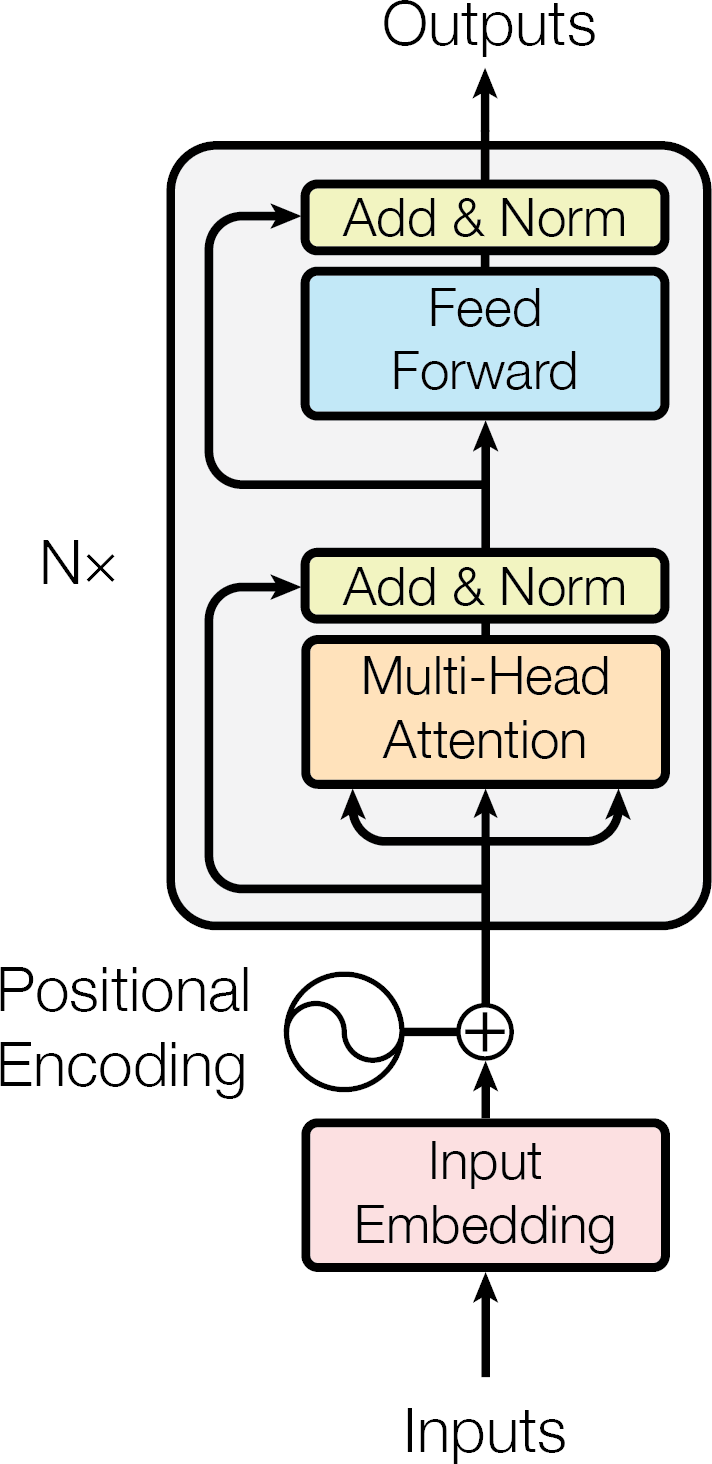
\includegraphics[width=\textwidth]{images/Transformer/TF_Encoder.png}

      \caption{Overview of the Transformer Encoder.}
      \label{fig:encoder}
    \end{subfigure}
    \hspace{0.2\textwidth}
    \begin{subfigure}{0.2\textwidth}
        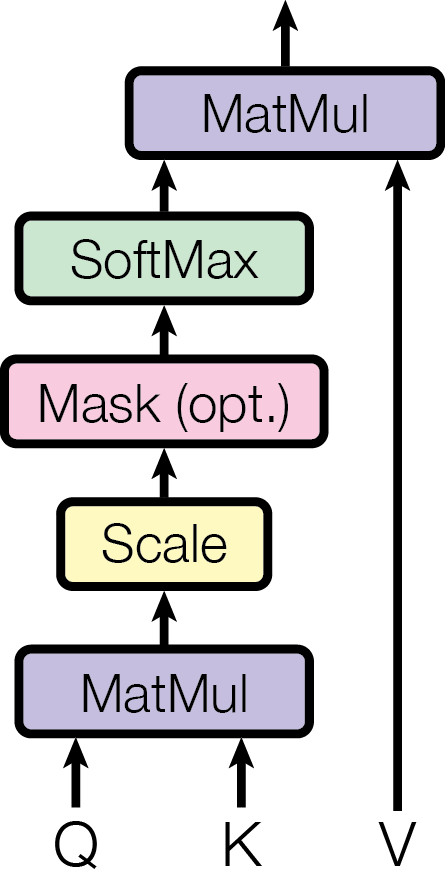
\includegraphics[width=\textwidth]{images/Transformer//AttentionHead.png}
        \caption{Attention Mechanism.}
      \label{fig:selfattention}
    \end{subfigure}
    \caption{Transformer Encoder Architecture. Figures taken from \cite{vaswani2017attention}.}
    \label{fig:transformer}
  \end{figure}

The idea of attention can be explained as follows: given a set of inputs, the model learns to assign a weight to each input based on its relevance to the 
task at hand.
This weighted sum of inputs is then used as a representation of the input sequence.\\

One of the most successful architectures for attention based sequence models is the Transformer developed by Vaswani, et al. \cite{vaswani2017attention}. In the paper, the transformer 
consists of an encoder and a decoder.\\

The Transformer architecture consists of an encoder and a decoder, each containing multiple layers of self-attention and feedforward neural networks. \\
In the self-attention layer, each input token is transformed into a query $Q$, key $K$, and value $V$ vector. 
The vectors $Q$, $K$ and $V$ are computed using a position wise feed forward network with ReLU activation:
\begin{equation}
    QKV = \text{ReLU}(x \ W_1 + b1)W_2 + b_2,
\end{equation}
where the same weights $W_n$ and biases $b_n$ are used for every input $x$ of the sequence. This is expected to be an advantage following the BIC argument from section \ref{COD}. 
These vectors are used to compute the attention weights between each pair of input tokens.
The resulting weighted sum of value vectors is used as the output of the self-attention layer.
The attention weights are computed as follows:
\begin{equation}
\text{Attention}(Q, K, V) = \text{softmax}\left(\frac{QK^T}{\sqrt{d_k}}\right)V,
\end{equation}
where $d_k$ is the dimensionality of the key vectors.
The softmax function normalizes the dot product of $Q$ and $K$, which represents the similarity between the query and key vectors.
The attention weights represent the importance of each value vector in the weighted sum. They can then be input to an MLP to compute the result.\\
 
Note with this setup, the model has no way to encode the relative position of the tokens, which is why a positional encoding is added along the sequence dimension, 
using sine and cosine functions, to break the symmetry.\\ 
In this thesis, we will use transformer encoder to model our neural networks. They only consists of self attention and the output MLP, as depicted in figure \ref{fig:transformer}. 
We will not describe the whole transformer architecture, 
as in this thesis we only make use of the encoder architecture.\\
One advantage of the Transformer architecture is that it does not suffer from the problem of vanishing or exploding gradients.
This is because the self-attention mechanism allows the model to directly access any input token, without the need for recurrent connections. Self attention type 
architectures have been shown to outperform recurrent networks on a number of sequence based tasks. For example they are used in the GPT-3 architecture, which has 
shown impressive results in natural language prediction \cite{brown2020language}. While they were developed for natural language tasks, they have 
shown promising results in a multitude of areas, including image generation, image classification, imitation learning and reinforcement learning.

% !TEX root = ../main.tex

\chapter{Related Work}
\label{chapter:RelWork}
Our work focuses on using search in inference time. Importantly, we consider \ac{mdp}s and \ac{pomdp}s where only a single observation is given. 
We assume some expert demonstrations and access to a sparse
reward of whether the task was successfully solved. \\

While sparse rewards and expert demonstrations are a key feature of our algorithm, it is generally applicable to deterministic \ac{mdp}s and deterministic \ac{pomdp}s. That is why we compare our 
findings to two state-of-the-art general purpose \ac{rl} algorithms, which we will develop in this section in detail, as we find it key to analyze experimental results. 
Another key aspect is imitation learning, which is why we include a state-of-the-art imitation learning algorithm in our baselines, which we will introduce in this section. \\

Furthermore, we will discuss current approaches that addresses parts of our setup. \\
We will first focus on imitation learning, then cover guided \ac{rl} with sparse rewards, and then
discuss how inference time search is used in current algorithms. Some of the presented approaches cover multiple requirements, so they cannot unambiguously be sorted into the provided categories.

\section{General Purpose Reinforcement Learning Algorithms}
\subsection{PPO}
\label{section:PPO}
Schulman, et al. \cite{PPO} introduce "Proximal Policy optimization" (PPO), which 
builds upon the ideas of Trust Region Policy optimization (TRPO) \cite{TRPO}. In TRPO, instead of the objective \ref{LPG}, a "surrogate" objective $L^{TRPO}$ is optimized 
with respect to a KL divergence constraint:
\begin{flalign}
        \text{optimize } L^{TRPO}(\theta) = \mathbb{E}_{(a, s, t) \propto \pi_{\theta}} \left[\frac{\pi_{\theta}(a|s)}{\pi_{\theta_{old}}(a|s)} A(s,a)\right] \\
        \text{subject to\ \ \ \ \ \ \ \ \ \ \ \ } \mathbb{E}_t[\text{KL}[ \pi_{\theta_{\text{old}}}(\cdot | s_t), \pi_{\theta}(\cdot | s_t)] ] \leq \delta
\end{flalign}
The core idea is to place a constraint on the distance between the new policy and the old policy. By doing so, 
too large update steps to the policy should be prevented, resulting in a more stable learning behavior. 
Recall the advantage estimator was defined as:
\begin{equation}
    A(s,a) = Q(s,a) - V(s).
\end{equation}
Plugging in the advantage estimator into \ref{reinf_update} gives the update rule:
\begin{equation}
    \nabla_{\theta} J(\pi_{\theta}) = \mathbb{E}_{(a, s, t) \propto \pi_{\theta}}[\nabla_{\theta} \mathrm{log}(\pi_{\theta}(a|s))A(s,a)]
\end{equation}
with the corresponding loss:
\begin{equation}
    \label{LPG}
    L^{\mathrm{PG}}(\theta) = \mathbb{E}_{(a, s, t) \propto \pi_{\theta}}[-\mathrm{log}(\pi_{\theta}(a|s))A(s,a)].
\end{equation}
Most common implementations of PPO use a stochastic policy, like in SAC, with the corresponding loss:
\begin{equation}
    \label{PPO_Loss_Reg}
    L^{\mathrm{PG}}(\theta) = \mathbb{E}_{(a, s, t) \propto \pi_{\theta}}[-\mathrm{log}(\pi_{\theta}(a|s))A(s,a)+\alpha \mathrm{log}(\pi_{\theta}(a|s))].
\end{equation}

In TRPO, ensuring the KL constraint requires a second order approximation to it. PPO is an on-policy algorithm that uses only first order approximations, while 
also making sure that the policy update does not change the policy too much. Instead of the hard KL constraint, it clips the gradient of the policy update within 
an $\epsilon$ region around the old policy.\\

Let
\begin{equation}
    r_t = \frac{\pi_{\theta}(a_t|s_t)}{\pi_{\theta_{old}}(a_t|s_t)}
\end{equation}

\begin{equation}
        L^{\mathrm{CLIP}}(\theta) = {E}_t \left[ \min \left(r_t(\theta) {A}_t, \text{clip} \left(r_t(\theta), 1-\epsilon, 1+\epsilon \right) {A}_t \right) \right].
\end{equation} \\

The algorithm aims to minimize $L^{\mathrm{CLIP}}(\theta)$ by doing gradient update steps:
\begin{equation}
    \theta_{i+1} = \theta_{i} + \alpha \nabla_{\theta} L^{\mathrm{CLIP}}(\theta_i).
\end{equation}\\

The pseudocode of the algorithm is shown in algorithm \ref{ppo_algo}.
\begin{algorithm}[h]
    \SetAlgoLined
    \begin{algorithmic}
    \For{$\text{iteration}=1,2,\dots$}{ \\
        \State Run policy $\pi_{\theta_\text{old}}$ in environment for $T$ timesteps\\
        \State Compute advantage estimates $\hat{A}_1, \dots, \hat{A}_T$\\
        \State optimize surrogate $L^{\mathrm{CLIP}}$ with respect to $\theta$. \\
        \State $\theta_\text{old} \gets \theta$
        }
        
    \end{algorithmic}
    \caption{PPO, actor critic style}
    \label{ppo_algo}

\end{algorithm}
Overall, PPO is a robust and effective algorithm for deep reinforcement learning, and has been successfully applied to a wide range of environments and tasks.\\

A GRU can be used in the recurrent implementation of PPO called Recurrent Proximal Policy optimization (RPPO) as analysed by Pleines, et al. 
\cite{RPPO}. Here the policy $\pi$ is defined on the history of observations and actions using a recurrent hidden state $h_t : o_{1:t} \times a_{1:t}$ with $\pi : o_{1:t} \times a_{1:t} \rightarrow \mathcal{R}$.
The adapted loss function from PPO is defined as:
\begin{equation}
    LC_t(\theta) = \widehat{\mathbb{E}}_t\big[\min\big(q_t(\theta)\widehat{A}_t, \text{clip}\big(q_t(\theta), 1 - \epsilon, 1 + \epsilon\big)\widehat{A}_t\big)\big] \tag{1}
\end{equation}
\begin{equation*}
    \text{with ratio} \quad q_t(\theta) = \frac{\pi_{\theta}(a_t \vert o_t, h_t)}{\pi_{\theta \text{old}}(a_t \vert o_t, h_t)}.
\end{equation*}
We will use RPPO as part of our baselines.


\subsection{TQC}
\label{section:TQC}
Arsenii Kuznetsov, et al. proposed "Truncated Mixture of Continuous Distributional Quantile Critics" (TQC) \cite{TQC_Paper} to compensate for the over estimation bias of critics in actor critic methods.\\
Empirically, the learned $Q$ function tends to overestimate the actual $Q$ value. We already saw one way to counter this bias by using the minimum value of 
two critics in the SAC algorithm \ref{SAC}. From a formal derivation of the overestimation bias by 
Thrun and Schwartz \cite{thrun1993issues} it is found that:
\begin{equation}
    \label{eq:overestimation}
    \begin{align}
        \max_a Q(s,a) = \max_a \mathbb{E}_{U}\left[Q(s,a) + U(a)\right] \leq \mathbb{E}_{U}\left[\max_a \left{Q(s,a) + U(a)\right}\right],
    \end{align}
\end{equation}
where $U(a)$ is action dependent random noise with zero mean. \\
The main idea of TQC is to learn the probability distribution of the $Q$ value, rather than approximating the expectation of the $Q$ value. 
It is then possible to drop the "right tail", meaning the highest quantile estimates for the $Q$ value, to lower the estimate.\\
Formally the goal is to approximate the random variable $Z^\pi(s,a):=\sum_{t=0}^\infty\gamma^tR(s_t, a_t)$, rather then 
$Q^\pi  := \mathbb{E}[Z^\pi(s,a)] = \mathbb{E}[\sum_{t=0}^\infty\gamma^tR(s_t, a_t)]$. This is done using quantiles.\\
The $k$th $M$-quantile of a distribution with random variable $X$ is defined as the the value $x$ for which the cumulative distribution function crosses $k/M$:
\begin{equation}
    Pr[X \leq x] \leq k/M
\end{equation}
with $M$ total quantiles. \\
Quantile regression is used to learn the values of the $M$ quantiles:
\begin{equation}
    \label{rho}
    \begin{align}
    L^{\tau_m}_{QR}(\theta^m) := \mathbb{E}_{\tilde{Z}\sim Z}\left[\rho_{\tau_m}(\tilde{Z}-\theta^m)\right],\\
    \quad \text{where} \quad \rho_{\tau_m}(u) = u({\tau_m} - I(u < 0)), \quad \forall u \in \mathbb{R}.
    \end{align}
\end{equation}
with ${\tau_m = \frac{2m-1}{2M}}, m \in [1, ...., M]$.\\
Let $\theta^m(s,a)$ be the approximation of the $m$-th quantile of $Q(s,a)$. The probability distribution $Z(s,a)$ can be approximated using $\theta^m$:
\begin{equation}
    Z_{\theta}(s,a) (v) = \frac{1}{M} \sum_{m=1}^M 1_{\theta^m(s,a) \geq v} | v\in\mathcal{R}.
\end{equation}
The temporal difference target can then be written as:
\begin{equation}
    y_i(s,a) := r(s,a) + \gamma \mathbb{E}_{s' \propto \mathcal{D}, a' \propto \pi(\cdot|s')}[\theta^i(s',a') - \alpha \log \pi_{\varphi}(a'|s')]
\end{equation}
with the target distribution
\begin{equation}
    Y(s,a)(v) = \frac{1}{N} \sum_{i=1}^N 1_{y_i(s,a) > v} | v \in \mathcal{R}
\end{equation}
$N<M$, where only the lowest N quantiles were used. \\
Finally this expression leads us to the loss function for the quantiles $\theta_m^{\psi}$ of Y:
\begin{equation}
    L_k(s,a;\psi) = \frac{1}{kN}\sum_{m=1}^{M}\sum_{i=1}^{kN}\rho^H_{\tau_m} \left(y_i(s,a) - \theta_m^{\psi}(s,a)\right),
\end{equation}
where $\psi$ denotes the parametrization of $\theta$.\\
From this we can find the entropy regularized policy loss function $J$:
\begin{equation}
    J_\pi(\phi) = \mathbb{E}_{D \propto \pi}\left[\alpha\log\pi{\phi}(a|s) - \frac{1}{M}\sum_{m=1}^{M}\theta_m^{\psi}(s,a)\right].
\end{equation}
In the TQC paper, they use N critics $\psi_n$. To keep the notation clean, we derived the main ideas using only one. An 
overview over the algorithm with N critics can be found in \ref{algo:TQC}.

\begin{algorithm}
    \caption{TQC Algorithm [\ref{algo:TQC}]}
    \label{algo:TQC}
    \begin{algorithmic}
        \State Initialize policy $\pi_{\phi}$, critics $Z_{\psi_n}$, $Z_{\psi_n}$ for $n \in [1..N]$\\
        \State Set replay $D = \emptyset$, $\beta = 0.005$\\
        \For{each iteration}{
            \For{each environment step, until done}{
                \State Collect transition $(s_t, a_t, r_t, s_{t+1})$ with policy $\pi_{\phi}$ \\
                \State $D \leftarrow D \cup {(s_t, a_t, r_t, s_{t+1})}$\\
            \EndFor}
            \For{each gradient step}{
                \State Sample a batch from the replay $D$\\
                \State $\phi \leftarrow \phi - \lambda{\pi} \hat{\nabla}{\phi}J{\pi}(\phi)$\\
                \State $\psi_n \leftarrow \psi_n - \lambda_Z \hat{\nabla}{\psi_n}J_Z(\psi_n), \text{for } n \in [1..N]$\\
                \State $ \overline{\psi_n} \leftarrow \beta \psi_n + (1 - \beta)\overline{\psi_n}, \text{for } n \in [1..N]$
            \EndFor\\}
        \EndFor\\}
        \State \textbf{return} policy $\pi_{\phi}$, critics $Z_{\psi_n}$
    \end{algorithmic}
\end{algorithm}
TQC achieves state-of-the-art performance in a wide variety of challenging tasks, like robotic manipulation in the OpenAI Gym environment \cite{1606.01540}, which makes it a fitting baseline 
for our experiments. It is specifically suited 
for off policy learning with a focus on exploration, in contrast to PPO, which was designed for on policy update steps.

\section{Imitation Learning}
\subsection{Generative Adversarial Imitation Learning}
Generative Adversarial Imitation Learning (GAIL) \cite{ho2016generative} is a key paradigm for efficient imitation learning that uses expert demonstrations in \ac{mdp}s. 
The main idea of GAIL is to disambiguate the reward signal from IRL by ensuring that every policy except the expert policy has a lower expected reward under the inverse reward function, given the expert 
demonstrations. Following, we will use a cost function $c \propto -r$, as it gives a natural optimum at $c=0$.\\

The entropy regularized IRL objective is written as:

\begin{equation}
    \label{proto_inf_ler_c}
    \pi_{\text{inv}}^* = \underset{c_{\text{inv}} \in \mathcal{C}}{\text{max}} \left( \min_{\pi \in \Pi} \left(- \text{H}(\pi) + \mathbb{E}_{\pi}[c_{\text{inv}}(s, a)] \right) - \mathbb{E}_{\pi_{\text{E}}}[c_{\text{inv}}(s,a)] \right),
\end{equation}
    
where $\text{H}(\pi)$ denotes the discounted causal 
entropy, $c_{\text{inv}}$ denotes the inverse cost function, $\mathcal{C}$ denotes the set of all possible cost functions and $\pi_{\text{E}}$ denotes the expert policy that is assumed to maximize the true cost function.
To find the cost function that fulfil the disambiguation requirement and optimizes equation \ref{proto_inf_ler_c}, a discriminator $D$ is learned, that tries to predict, if a transition is 
sampled from the expert policy or the learned policy.  

Formally the GAIL objective is defined as:
\begin{equation}
    J(\rho_{\pi_{\theta}}, D_{\omega}) =  - \lambda \bar{\text{H}}(\rho_{\pi_{\theta}} ) + \mathbb{E}_{\pi_{\theta}}\left[ \text{log}(D_{\omega}(s,a))\right] + \mathbb{E}_{\pi_{\text{E}}}\left[ \text{log}(1 - D_{\omega}(s,a))\right],
\end{equation}
where $\theta$ and $\omega$ are the parameters of the generator and discriminator, respectively, 
$\lambda$ controls the trade-off between the similarity to the expert trajectories and the entropy of the policy and $D_{\text{KL}}(\cdot || \cdot)$ denotes the Kullback-Leibler divergence. \\
Intuitively discriminator tries to distinguish between the expert and generated trajectories, while the generator tries to produce trajectories that are indistinguishable from those of the expert.\\

Overall, GAIL is a state-of-the-art imitation learning algorithm which is able to learn complex behavior with limited expert demonstrations. It shows outstanding 
asymptotical performance with respect to the amount of expert demonstrations, which is why we will use it as a baseline in our experiments.\\ 
A downside is that it requires a high number of environment interactions to train the discriminator and actor, as stated by the authors. A more detailed derivation of the algorithm and theoretical 
bounds can be found in appendix \ref{app:GAIL}.


\subsection{Generative Adversarial Imitation Learning in \ac{pomdp}s}
\label{GAIL_POMDPS}
In this section, we will describe an imitation learning approach based on GAIL, that handles \ac{pomdp}s.\\
The GAIL algorithm assumes access to the actual state $s_t$ of the MDP. Gangwani, et al. \cite{gangwani2019learning} 
extend the GAIL paradigm to work on \ac{pomdp}s. To do so, they introduce a network $B_{\phi}(o_{\leqt}, a_{\leqt}) = b_{t, \phi}$ that aims to approximate a 
representation of the belief state $b_t$. Using $b_{\phi}$ instead of $s$ the new objective is:
\begin{equation}
    \min_{\phi,\theta}\max_{\tilde{\omega}} &\mathbb{E}_{(b,a)\sim\mathcal{M}_{\text{E}}}[\log D_{\tilde{\omega}}(b_{\phi},a)] + \mathbb{E}_{(b,a)\sim\pi,\mathcal{T}}[\mathrm{log}(1-D_{\tilde{\omega}}(b_{\phi},a))]
\end{equation}
with the corresponding imitation loss 
\begin{equation*}
    \mathcal{L}^{\text{IM}}(\phi) := D_{\text{JS}}(\theta,\phi) \approx \tilde{E}_{(h,a)\sim \mathcal{M}_\text{E}}[\log D^*(b_\phi(h),a)] + \tilde{E}_{(h,a)\sim \pi_\theta(a|b_\phi(h)),\mathcal{T}}[\mathrm{log}(1 - D^*(b_\phi(h),a))], 
\end{equation*}
where $D^*$ denotes the optimal discriminator. 
The authors include three regularization losses to improve the expressiveness of $b_{\phi}$. For example:
\begin{equation}
    \mathcal{L}^f(\phi) = \mathbb{E}|| o_{t+k} - g(b_t^\phi, a_{t:t+k-1})||_2^2,
\end{equation}
where g is a learned stochastic unimodal gaussian with learned mean and fixed variance.\\

Intuitively, this term seeks to impose, that the belief state $b_t$ is indeed a sufficient statistic for the 
\ac{pomdp}, by forcing the model $b_{\phi}$ to learn a representation that can predict future observations given future actions. The superscript $f$ of the regularization loss means forward. 
In a similar way, there is an inverse regularization $i$, which looks k steps into the past. Additionally, the authors propose an action regularization $a$ which tries to reproduce the actions that were 
taken, given the initial belief state and the subsequent observations. With all three regularization losses, the total loss function for the believe module is:
\begin{equation}
    L(\phi) = L^\text{IM} + \lambda_1 L^\text{f} + \lambda_2 L^\text{i} + \lambda_3 L^\text{a},
\end{equation}
where $\lambda_i$ are the weights for the respective regularizers. \\
The approach is superior to GAIL with frame stacking and can also improve upon GAIL with recurrent networks for the discriminator and the actor, though the margins are small in some cases. The advantage 
of their approach is, that the believe state representation will be expressive following their regularizers. However, they use an $L_2$ distance error between the predictions and the observations. In most environments, 
the observations are high dimensional and include redundant or unnecessary information that will be hard to learn. This forces the network to allocate capacity that is not directly used to 
optimize the overall objective. Moreover, as GAIL, this approach suffers from bad sample efficiency with respect to environment interactions and cannot make use of a reward signal from the environment. 

\subsection{Single Observation Imitation Learning in \ac{pomdp}s}
Simon Stepputtis, et al. \cite{stepputtis2020languageconditioned} propose a method for robot manipulation tasks that takes 
into account natural language instructions. 
In this setup, there is only one observation per trajectory, namely the task description and the first image of the environment.
The proposed method involves using a neural network to map natural language instructions to 
corresponding robot actions, using a GRU to unroll the trajectory. The authors also introduce a novel dataset of language-conditioned robot manipulation tasks, which we will use to evaluate 
and compare the performance of our method in pure imitation learning settings.\\ 
The experimental results demonstrate the effectiveness of their approach in inferring and executing trajectories for robot manipulation 
tasks when language instructions are given. A more detailed overview of the method, dataset and benchmark can be found in appendix \ref{LCILRM}.\\


\section{Sparse Reward}
\label{sec:HER}
Learning with sparse rewards is challenging in a high-dimensional action and observation space, as nearly all trajectories will have a reward of 0.
Until, by chance, a successful trajectory is found, the agent has to blindly guess. To overcome this problem, Marcin Andrychowicz et al. \cite{andrychowicz2018hindsight} 
propose "Hindsight Experience Replay".\\

The algorithm works by generating new goals for a given trajectory based on the states that were actually reached.
Specifically, consider the problem of finding a policy $\pi(a|o, g)$ given observation $o$ and goal $g$.
If the goal is reached, the reward is 1. Given a state at time step $t$ $s_t$ and a goal state $g$, with $s_t \neq g$,
the reward for the state is $r(s_t|g) = 0$, which does not provide much information for the policy.
To use the information of which state was actually reached by the trajectory, a new goal is constructed $g' = s_t$. Using this, the new reward is $r(s_t|g') = 1$.
The agent can then learn from these hindsight goals, which can provide more frequent rewards and enable faster learning. An additional advantage of HER is that it is agnostic with respect to the learning algorithm, as it only provides additional trajectories for the replay buffer.

Overall, HER is a powerful algorithm that addresses the problem of sparse rewards in \ac{rl} by leveraging hindsight. It has been successfully applied to a wide range of tasks, 
including robotic manipulation, locomotion, and game playing, and has shown superior performance compared to standard \ac{rl} algorithms.\\

A downside of HER is that it requires the inverse function $g(s)$, meaning from a visited state, the goal must be reconstructible. This is not always given.
Consider the goal of not driving into a vehicle or a goal expressed in natural language. \\

Another approach is to use curiosity for better exploration in sparse reward settings.\\

One common approach similar to Pathak et al \cite{pathak2017curiositydriven} to curiosity-driven exploration is to use an intrinsic reward function, which is designed to 
measure how surprising or informative a particular 
state or action is to the agent. \\

By incorporating this intrinsic reward signal into the overall \ac{rl} objective, the agent is encouraged to explore areas of the environment that are 
unexpected or uncertain, which can lead to discovering new strategies or behaviors that improve its performance. This approach has been shown to be effective in a variety of 
domains, including robotics, gaming, and natural language processing.\\

This approach is very general and can be added as an addition to classical reinforcement learning.

\subsection{Guided Reinforcement Learning with Sparse Rewards}
\label{sec:rel_work_finetuning}
With guided \ac{rl} we refer to expert knowledge that is provided to the algorithm, for example with expert demonstrations.
Mel Vecerik et al. \cite{vecerik2018leveraging} describe a priority 
sampling algorithm in combination with deep deterministic policy gradient (DDPG). The probability with which a 
training sample is chosen from the replay buffer is defined as: 
\begin{equation}
    P(i) = \frac{p_i^\alpha}{\sum\limits_{k} p_k^\alpha}
\end{equation}
with 
\begin{equation}
    p_i = \delta_{i}^2 + \lambda \lvert \nabla_a Q(s_i, a_i \vert \theta_Q) \rvert^2 + \epsilon + \epsilon_{D}.
\end{equation}
Here $\delta_{i}$ is the temporal difference error, $\lambda$ is used to weigh the importance of the sample i with respect to the loss of the actor, 
$\epsilon$ is a small constant to ensure every transition is chosen with probability $p_i > 0$, and $\epsilon_D$ is a positive constant applied for expert transitions.\\
The idea behind this importance sampling algorithm is to amend the priority experience replay probability as developed by Schaul et al. \cite{schaul2016prioritized} 
with a constant $\epsilon_{D}$ for expert demonstrations to make the policy converge faster to the expert behavior. In priority experience replay, more rare 
experiences are chosen more likely to use the data in the replay buffer more efficiently. Moreover, they use a combination between $n=1$ temporal difference and 
$n=N > 1$ temporal difference to get better estimations for rewards that are in the distant future, as they assume sparse rewards.\\
The effectiveness of the approach is demonstrated by comparing the performance of their importance sampling algorithm with sparse rewards to a standard DDPG 
implementation using no expert demonstration but dense reward. The authors find that their approach can learn faster then standard DDPG with 100 expert 
demonstrations on a challenging robotic insertion task.\\ 
A problem with this approach is, that the critic assumes the temporal difference error approximates the distribution induced by the policy $\pi_{\theta}$, but by 
mixing in expert demonstrations, the expected $Q$ value will be higher, then that of the policy $\pi_{\theta}$. This overestimation can lead to poor performance. 
To counter this, the authors include a term to "weigh the update to the network" $w_i = \frac{1}{N} \cdot \frac{1}{P(i)}$. This term however is inversely proportional to the 
probability of choosing a transition and thus counter acts the improvement rate towards expert behavior. 

\section{Search in Inference Time}
\subsection{Discrete Action Space}

Schrittwieser et al. \cite{MUZero} describe a search based algorithm for discrete action spaces called MuZero. It is designed to achieve state-of-the-art performance 
in a wide range of games without any prior knowledge of the game rules, unlike its predecessor AlphaGo and AlphaZero, which relied on a hand-crafted 
domain-specific algorithm. MuZero learns to play games by combining deep neural networks with \ac{mcts} to plan and evaluate its actions. 
It does not have access to the game states, but only to observations covering a limited amount of information in a \ac{pomdp} setting.
To plan ahead, it predicts the expected rewards $r_{t:T}$ for a proposed action sequence $a_{t:T}$ given a history of observations $o_{1:t}$.\\
For the search, the planner needs access to a model predicting the reward after n steps. To learn this model, the authors use an end-to-end trained recurrent neural network, which 
compares it's prediction to the actual rewards from the environment. The prediction and search proves to be crucial for the performance of MuZero.\\ 
While MuZero achieves state-of-the-art performance on the challenging ATARI 57 benchmark, it requires discrete actions for the \ac{mcts} based algorithm.

\subsection{Continuous Action Space}
\label{sec:mctsca}
Lee et. al \cite{Lee_Jeon_Kim_Kim_2020} develop a possible way to relax the requirement of a discrete action space of the MuZero algorithm. 
The main idea is to separate 
the \ac{mcts} into two phases, a coarse phase, where actions from the action space are coarsely sampled and a fine tuning phase, where the actions are tuned, using the continuity of the action space.\\
To tune the actions, the gradient of the reward with respect to the policy is taken, where $\pi_t(a|t)$ represents the policy for action at time step t. 
Formally, the gradient can be written as $\Delta \pi_t = \frac{\partial V (s_t, \pi_{t:T})}{\pi_{t}}$. Given a differentiable model of the environment, their algorithm can 
find solutions to tasks with no prior training. The authors demonstrate their approach on several robot 
benchmarks, where it can match or surpass the performance of pretrained SAC, given 5 seconds computation time per action.\\
While this approach uses planning on continuous action space, it relies on a given model of the environment to approximate the gradients and perform the \ac{mcts}.

% !TEX root = ../main.tex
\chapter{Problem Statement}
\label{chapter:Problem}
In this thesis, we aim to develop an algorithm that uses search in inference time on a continuous action space. 
A focus is to efficiently leverage expert demonstrations to solve environments with sparse feedback signals. We will use fixed horizon continuous 
deterministic \ac{mdp}s with sparse rewards and fixed horizon deterministic \ac{pomdp}s, where only a single initial observation is provided, along with sparse rewards. \\

Formally we define a continuous fixed horizon \ac{sopomdp} as a tuple
$$\langle S,A,T,O,R,G, h  \rangle,$$
where $S$ is the state space, $A$ is the action space, $T$ is the transition 
function, $O$ is the observation space, $R$ is the reward function, $G$ is the set of states for which the reward is $1$, and $h$ is the time horizon.\\ 
At each time step $t=1,...,T$, the agent has access to the observation $o_t = s_1$ and selects an action $a_t$.  
It then receives a 
reward $r_t\in \{0,1\}$, where 
\begin{cases}
    r_t = 0 \quad  |t < T\\
    r_T = 1 \quad  |g \in \{ s_t \}\\
    r_T = 0 \quad \text{else.}
\end{cases} \\
Intuitively, the reward is $1$ only if a goal state was reached along the trajectory. We also relax the single 
observation constraint, where the agent receives the state of the environment after each step: $o_t = s_t$, as defined for \ac{mdp}s. The rest of the setting is equal.\\

The goal of our algorithm is to learn a policy $\pi(a_t|o_{1:t}, a_{0,...,t-1})$ that maximizes the expected cumulative reward over a trajectory of length $T$ given 
some expert trajectories $D_{\text{expert}}$. 
That is, we seek to solve the following optimization problem:

\begin{equation}
\max_{\pi} \mathbb{E}_{\pi}[r_T]\quad \text{given}\quad D_{\text{expert}}
\end{equation}

where the expectation is taken over trajectories of length $T$ induced by the policy\\ $\pi(a_t|o_1, a_1, ..., a_{t-1})$.\\

Our algorithm aims to be sample efficient with respect to both expert trajectories and environment interactions. \\

Currently, \ac{gail}, a state of the art \ac{il} algorithm, has good asymptotical performance with respect to the number of expert trajectories, but is not sample efficient 
with respect to environment interactions during train time. Moreover, it does not make use of reward signals from the environment but only relies on the expert demonstrations.\\ 

An approaches to leverage expert demonstrations by sampling them with higher priority \cite{vecerik2018leveraging} has limited convergence rate towards expert behavior and is dependent on additional hyperparameters. 
An additional problem with mixing expert demonstrations and reinforcement data in actor critic algorithms is, that they induce two different distributions, one from the expert and one from 
the learner. This leads to overestimation by the critic, further hindering the learning process. \\

Apart from the expert demonstrations, critics in actor critic methods generally overestimate the expected reward. \ac{tqc} \cite{TQC_Paper} aims to solve this issue by learning the 
probability distribution of the expected reward and ignore the highest tail of it. While it shows good performance in \ac{rl} environments 
it is also reliant on additional hyperparameters 
specifying the coarseness of the learned probability distribution and the cutoff point. To solve this problem , we aim to develop a critic that is inherently unbiased using transitions from expert demonstrations 
and \ac{rl}.\\

A third difficulty with actor critic methods is that the update step of the policy must be carefully tuned. Apart from the general overestimation of the critic, it has a variance in the estimate, 
as it is a learned function approximator. The more the policy is changed in an update step, the less accurate the prediction of the critic. To solve this problem, \ac{ppo} ensures limited change of the policy 
between update steps, making it more robust. The trade-off is less exploration compared to \ac{tqc}. To have good exploration 
and ensure stable improvement without the need of extensive hyperparameter tuning, we aim to use inference time search to find and apply candidate solutions, which can vary widely from the 
proposed trajectory of the actor, without changing the actor itself. \\

While there are approaches using search in inference time, they either require discrete action spaces \cite{MUZero} or a given differentiable model of the environment \cite{Lee_Jeon_Kim_Kim_2020}. 
In our approach, we 
don't make the assumption that such a model is provided, as in real world robotic applications, this is typically not the case.\\

We are interested in investigating the effectiveness of our search paradigm, which requires a learned weakly grounded model of the environment. We first develop the approach 
for single observation environments, 
as they don't provide additional information during the trajectory is rolled out, making the prediction of the whole environment dynamics crucial. We will then relax the constraint to the typcial 
\ac{mdp} setting.

% !TEX root = ../main.tex

\chapter{Methodology}
\label{chapter:Methodology}
We identify two main challenges with the single observation sparse reward setup. \\

\section{Curse of Dimensionality}
\label{COD_AC}
As introduces in \ref{COD}, the evidence for a model scales approximately inversly proportinal to the exponent of the dimension on which it acts. In MDPs, the 
actor $\pi$ acts on the observation space and returns an action from the action space. A probabalistic actor defines a probability distribution on the set 
of actions $\mathcal{A} \in \mathcal{R}^m$ and observations $\mathcal{O} \in \mathcal{R}^n$ as $\pi(a|o) = \frac{p(a,o)}{p(o)}$. 
Thus the dimension on which the actor acts on, is $n \times m$ with $\pi:\mathcal{R}^m \times \mathcal{R}^n \rightarrow \mathcal{R}$.\\
Similarely, the critic $Q$ usually defines a function on $\mathcal{A}$ and $\mathcal{O}$ to the comulative discounted expected value 
$Q:\mathcal{R}^m \times \mathcal{R}^n \rightarrow \mathcal{R}$, while TQC defines the critic as a quantile distribution: 
$Q:\mathcal{R}^m \times \mathcal{R}^n \rightarrow \mathcal{R}^k$ with $k$ quantiles.\\
We have shown in \ref{POMDP}, that in a POMDP, the observation space grows linear in time. Together with the result from \ref{COD} we conclude, that we have 
exponentially less evidence with sequence length $T$ for our model in the POMDP setting.\\
To counter this problem, we want to get rid of the time dependency of the belief state. To do this, 
we make the observation, that our case with the single observation at the beginning is a special case of a POMDP. Usually, 
we need to know all previous obervsations, as they can give us additional information about the believe state. However, as we don't have subsequent information 
after the initial observation, the only knowledge we have to include to calculate our believe state are the actions, that the policy took. As introduced in \ref{pomdp_bayes}, the optimal believe state 
update in the general POMDP case using bayes theorem is given by:
\begin{equation}
    b_{t+1}(s') = \frac{\mathcal{Z}(s', o_{t+1}) \sum_{s \in \mathcal{S}} \mathcal{T}(s, a_t, s') b_t(s)}{\sum_{s'' \in \mathcal{S}} \mathcal{Z}(a_t, s'', o_{t+1}) \sum_{s \in \mathcal{S}} \mathcal{T}(s, a_t, s') b_t(s)}
\end{equation}
. In our case, we can rewrite this as:
\begin{equation}
    b_{t+1}(s') = \frac{\mathcal{Z}(s', o_{0}) \sum_{s \in \mathcal{S}} \mathcal{T}(s, a_t, s') b_t(s)}{\sum_{s'' \in \mathcal{S}} \mathcal{Z}(s'', o_{0}) \sum_{s \in \mathcal{S}} \mathcal{T}(s, a_t, s') b_t(s)}
\end{equation}
. $\mathcal{Z}(s'', o_{0})$ is constant for $t>0$, so we get:
\begin{equation}
    b_{t+1}(s') \propto \sum_{s \in \mathcal{S}} \mathcal{T}(s, a_t, s') b_t(s) \quad | t > 0
\end{equation}
\begin{equation*}
    b_{0}(s') \propto \mathcal{Z}(s', o_{0})
\end{equation*}
. If we assume a deterministic policy $\pi(a|b) \rightarrow a_{\pi}(b)$, the update step can be written as:
\begin{equation}
    b_{t+1}(s') \propto \sum_{s \in \mathcal{S}} \mathcal{T}(s, a_{\pi}(b_t), s') b_t(s)
\end{equation}
. By using this update step recursively until we get to $b_{0}$, we see, that the believe state at time $t$ only depends on the initial observation $o_0$
the transition probability $\mathcal{T}$ and the number of recursion steps $t$. Using this insight, we can rewrite the belief state at timestep $t$ like:
\begin{equation}
    b_{t+1}(s') \propto \mathcal{Z}(s_0, o_{0}) \mathcal{T}(s_0, s', t)_{\pi}
\end{equation}
, where $\mathcal{T}(s_0, s', t)_{\pi}$ indicates that the normalized transition function depends on the timestep $t$ and policy $\pi$.\\
With this formulation, we can rewrite the policy 

\begin{equation}
    \pi(a|b) : \mathcal{R}^m \times \mathcal{R}^{n T} = \pi(a|o_0, t): \mathcal{R}^m \times \mathcal{R}^{n} \times 1.
\end{equation}
We call this a strong inductive belief state bias for the single observatino POMDP, as it forces the assumption of a deterministic and constant policy $\pi$. 
In our method, we implement a weak inductive bias, which is motivated by this observation: We use transformer encoder type architecture, which inputs are 
the repeated initial observation plus a positional encoding. We then use a single pass through the network, which means it does not work autoregressively and 
relies less on former actions to determin action at time point $t$. We test this hypothesis by using baselines that have the strong inductive bias, as well as 
using a recurrent policy.\\ 
Another benfit of computing the whole trajectory in one pass is that the independent and identically distributed (i.i.d.) input data 
assumption underlying supervised learning methods is not broken. The assumption states, that we don't expect a different data distribution durng infernece time 
then during train time, which generally does not hold for imitation learning, as the distribution of data seen during inference depends on the policy. 
However, by computing the whole trajectory at once, the input data is distributed according to the initial state of the POMDP, which is independent of 
the policy, thus the i.i.d. assumption holds.\\

\section{Update Error}
\label{inference_time_planning}
As we only have a single observation, our model has to learn the dynamics of the MDP in order to predict the reward signal at time point $t > 1$. In \cite{NEURIPS2020_b5c01503} 
it has been shown, that learning a transition model for an mdp has a quadratic error bound in $\gamma$ thus we expect quadratic error with the length of the horizon. 
However, we identify that this challange also grants us a unique improvement over previous actor critic methods. By predicting whole sequences of actions at once, 
we show that we can eliminate errors in the update step of the actor and critic.\\

\subsection{Critic}
\label{sec:AC_Critic}
To train the critic in actor critic mehtods, we can either use on policy data as in PPO \ref{section:PPO}, which is not sample efficient, as only the data collected 
in the current episode is used for training, or we can use off policy data as in TQC \ref{section:TQC}, where the critic has an overestimation bias. This 
leads to sub optimal data usage and the reliance on an addtional hyper parameter. We find that in our setup with a single observation, we can use all data 
collected without introducing a bias on the critic. \\
Recall that the overestimation bias comes from the reliance on the estimation of the $Q$ value for the bootstrapped temporal difference target \ref{eq:overestimation}:
\begin{equation}
    \label{eq:TD_Methodology}
    J_{\theta}(\pi) = \mathbb{E}_{a,a' \propto \pi, s' \propto T(s,a,s')}(r(a,s) + \gamma Q_\theta(a', s') - Q_\theta(a,s))^2
\end{equation}
, where the estimator is $Q_\theta(a', s')$. We propose to use a whole sequence critic $C_{\text{whole sequence}}$, which predicts all immediate rewards given a current observation 
and the planned action sequence for the whole trajectory:
\begin{equation}
    C_{\text{whole sequence}}(t, o, a_{1, ..., T}) = \mathbb{E}_{s_t \propto \tau_t}\left[r(a_t, s_t)\right]
\end{equation}
, where $\tau_t$ indicates the sequence until timestep $t$. 
The objective function is then defined as 
\begin{equation}
    J_\theta = \mathbb{E}_{o, a_{1, ..., t}, r_{1, ..., t}}\left[\sum_t(c_t - r_t)^2\right]
\end{equation}
. This is an unbiased estimate of the expected rewards at time step t following trajectory $a_{1, ..., t}$ and observation $o$, as it is simply the empiciral distribution 
over the rewards. Because the 
first observation is all the information we have during inference time, we find this aproach to be well suited for our setup.\\

Next we want to show that the wohle sequence critic can be used to find an optimal policy. 
To do this, we show the critic learns a proper value equvialent model of the POMDP. Recall the defining property of a proper 
value equvivalent model $m'$ for a model $m$ is defined in \ref{eq_kthVE} as:
\begin{equation*}
   \lim_{k \rightarrow \infty} \left(\mathcal{T}^{m'}_{\pi}(V)\right)^k = \lim_{k \rightarrow \infty} \left(\mathcal{T}^{m}_{\pi}(V)\right)^k
\end{equation*}
\begin{equation}
    = V_{\pi}.
\end{equation}
As we have argued above, the critic learns an unbiased estimate of the rewards $r_t$ given an action sequence. Using this, we can compute the value function for 
any action sequence $a_1, ..., a_T$ induced by a policy $\pi$:
\begin{equation*}
    V_{\pi}(s) = \mathbb{E}_{a_{1:T}, s_{1:T} \propto \pi, m}\left[\sum_{t=0}^{\infty} \gamma^t r_t \mid s_0 = s\right].
\end{equation*}
As it has been shown by Christopher Grimm et. al \cite{grimm2021proper}, a policy that is optimal with respect to a proper value equivalent model $m'$ is optimal 
in the actual POMDP with model $m$. We conclude, that our whole sequence critic is suited to learn an optimal policy.

\subsection{Actor}
\label{sec:AC_actor}
All parametrized actor critic mehtods are technically speaking off policy, as the critic value is bootstrapped with estimates sampled from former policies $\pi_{old}$ during the training process. 
Once the actor is updated, the 
critic target moved, on which the actor was updated. Intuitively, when the policy is changed to choose a different action at time point $t$, it might also change 
the policy to choose different actions at 
all subsequent time points, which changes the value function. \\

We assume this update instability is specifically challenging in our one observation environment, as the policy does not 
get updates of the state of the environment it is currently in. \\
Formally, define the objective function $J(\phi, \theta(\phi)) = \mathbb{E}_{\tau \propto \pi(\phi)}\left[Q_{\theta(\phi)}\right]$ for actor critic methods 
as the function we whish to optimize to learn the optimal policy. While there are other choices, like using the value estimate $V$ instead, the general argument holds.\\
$Q_{\theta(\phi_i)}$ indicates the $Q$ function for policy $\pi_{\phi_{i}}$ parametrized by parameters 
$\theta(\phi_i)$. For example, DDPGs policy update rule \ref{AC_general_update} is written as:
\begin{equation}
    \nabla_{\phi} J(\phi, Q(\theta(\phi))) = \mathbb{E}_{\tau \sim p(\tau | \pi_{\phi})} \left[\nabla_{\phi} \log \pi(a_t|s_t;\phi) Q_{\theta, \pi_\phi}(a_t, s_t) \right].
\end{equation}
. Note that generally, we do not have access to $\theta(\phi)$, but only an approximation given the limited data we have collected. Let us denote the actual 
$Q$ function we have as $Q(\theta(\phi) + \epsilon)$, where $\epsilon$ indicates an error between the optimal parameters and the actual parameters.
Let us now for simplicity assume, that $\phi$ and $\theta$ are one dimensional. A generalisation to n dimensions is straight forward. We want 
to estimate the update error to $\pi$ from the objective $J$. The proper derivative is given by:
\begin{equation}
    \nabla_{\phi} J(\phi, \theta(\phi)) = \frac{J(\phi + \delta \phi, \theta(\phi + \delta \phi)) - J(\phi, \theta(\phi))}{\delta \phi} + \mathcal{O}(\delta)
\end{equation}
with 
\begin{equation}
    J(\phi + \delta \phi, \theta(\phi + \delta \phi)) = J(\phi, \theta(\phi)) + \left[ 
        \frac{\partial J}{\partial \phi} + \frac{\partial J}{\partial \theta} \frac{\partial \theta}{\partial \phi}
    \right] \delta \phi  + \mathcal{O}(\delta^2)
\end{equation}
, where we used the chain rule and Taylor's theorem. 
We can express this in terms of the parametrs $\theta(\phi) + \epsilon$:
\begin{equation}
    \nabla_{\phi} J(\phi, \theta(\phi)) = \nabla_{\phi} J(\phi, \theta(\phi) + \epsilon) - \nabla_{\phi} J(\phi, \theta(\phi)) + \nabla_{\phi} J(\phi, \theta(\phi))
\end{equation}
\begin{equation*}
    = \nabla_{\phi} J(\phi, \theta(\phi)) + \epsilon_{\nabla_{\theta}}
\end{equation*}
. Note that $\nabla_{\phi} J(\phi, \theta(\phi) + \epsilon)$ is not a properly defined derivative. To rigorously capture the stochastic dependence of $\theta(\phi)$ 
given a dataset $\mathcal{D}^n$ with $n$ transitions, 
we could formulate $\theta(\phi)|\mathcal{D}_n$ as n boundary conditions. Together with a suitable regularizor, we can then find $\theta_{\epsilon, n}(\phi)$. We omit 
this step, as we are only interested in the fact that there is an error, not the exact value of it.\\
In actor critic policy updates, $\theta$ is assumed a constant, thus the actor derivative 
$\widetilde{\nabla}_\phi J$ of $J$ is given by:
\begin{equation}
    \widetilde{\nabla}_\phi J(\phi, \theta) =  \frac{J(\phi + \delta \phi, \theta) - J(\phi, \theta)}{\delta \phi} + \mathcal{O}(\delta)
\end{equation}
. 
Again using $\theta(\phi) + \epsilon$ we get:
\begin{equation}
    \widetilde{\nabla}_\phi J(\phi, \theta + \epsilon) = \widetilde{\nabla}_\phi J(\phi, \theta) + \epsilon_{\widetilde{\nabla}_{\theta}}
\end{equation}
We can now derive the update error in the actor update:
\begin{equation}
    \label{equation:general_update_error}
    \nabla_{\phi} J(\phi, \theta(\phi)) - \widetilde{\nabla}_\phi J(\phi, \theta) = \nabla_{\phi} J(\phi, \theta(\phi) + \epsilon) - \epsilon_{\nabla_{\theta}} - \widetilde{\nabla}_\phi J(\phi, \theta(\phi) + \epsilon) + \epsilon_{\widetilde{\nabla}_{\theta}}
\end{equation}
\begin{equation*}
    = \epsilon_{\widetilde{\nabla}_{\theta}} - \epsilon_{\nabla_{\theta}} + \frac{\partial J}{\partial \theta} \frac{\partial \theta}{\partial \phi}
\end{equation*}
. We will call $\epsilon_{\widetilde{\nabla}_{\theta}} - \epsilon_{\nabla_{\theta}}$ the  \textbf{function approximator error}. \\
Recall that $J(\phi, \theta(\phi)) = \mathbb{E}_{\tau \propto \pi(\phi)}\left[Q_{\theta(\phi)}\right]$, so the partial derivative $\frac{\partial J}{\partial \theta} = 1$, 
as the expectation commutes with the derivative. This leaves us with estimating $\delta \frac{\partial \theta}{\partial \phi}$. Again using taylor's theorem, we get 
\begin{equation}
    \label{dist_shift_error}
    \delta \frac{\partial \theta}{\partial \phi} = \theta(\phi + \delta) - \theta(\phi) + \mathcal{O}(\delta).
\end{equation}
We will call this error the \textbf{distribution shift error}. \\
While this derivation assumes direct policy gradient to update the actor, other actor critic policy update methods like the minimisation of a KL divergence as 
proposed is SAC will rely on simlar gradients in there update step (\cite{haarnoja2018soft}, equation 13).

\subsubsection{Distribution Shift Error}
\label{dist_shift_error_section}
From \ref{dist_shift_error} we see, that the error of the update of $\pi$ is proportinal to the change in the 
expected value $J(\pi)$. Using our whole sequence critic $C$, this error is zero. \\ 


Recall when we write $\theta(\phi)$ we mean $Q_{\theta}(a,s|\pi_{\phi})$:
\begin{equation*}
    Q_{\theta}(a,s|\pi_{\phi}) = \mathbb{E}_{(a_t \propto \pi_{\phi}(s_t), s_t \propto T(s_{t-1}, a_{t-1}, s_t))|a_0=a, s_0=s}\left[\sum_t \gamma^t r(a_t, s_t)\right]
\end{equation*}
from that we get
\begin{equation}
    Q_{\theta }(a,s|\pi_{\phi + \delta}) - Q_{\theta}(a,s|\pi_{\phi}) != 0 
\end{equation}
\begin{equation*}
    \text{ if } \pi_{\phi + \delta}(a|s) != \pi_{\phi}(a|s)
\end{equation*}
except for degenerate cases. We propose a whole sequence actor, where, given an observation, the actor proposes the whole sequence of actions it will 
take. We use these as input for the whole sequence critic, as discussed in the last section. 
Recall $C_{\text{whole sequence}}$ is defined on an observation $o$ and a 
sequence of actions: 
\begin{equation}
    (a_{1,...,T}) \propto \pi_{\text{whole sequence}}(a_{1,...,T}|o)
\end{equation}
\begin{equation*}
    C_{\text{whole sequence}}(t, o, a_{1,...,T}) = \mathbb{E}_{s_t \propto \tau_t}\left[r(a_t, s_t)\right]
\end{equation*}
, where $\tau_t$ indicates the trajectory until timestep $t$ and $c_{\text{whole sequence}}(t, o, a_1, ..., a_T)$ is the expected reward at time step $t$. \\
We can now see that, as there is no dependency of $C$ on $\pi$, the distribution shift error \ref{dist_shift_error} is zero. 

\subsubsection{Function Approximation Error}
\label{func_app_error}
Recall the function approximator error $\epsilon_{\widetilde{\nabla}_{\theta}} - \epsilon_{\nabla_{\theta}}$ in \ref{equation:general_update_error} was 
derived from the observation, that our $\theta(\phi)$ is underdetermined 
given limited data $\mathcal{D}^n$. \\
Intuitively, even if the distribution shift error is zero, meaning we knew perfectly the value 
$C((t, o, a_{1,...,T}) \in \mathcal{D}^n)$ of a given action sequence, we don't know the value of an arbitrary action sequence
$C((t, o, a_{1,...,T}), o \in \mathcal{D}^n, a_{1,...,T} \notin \mathcal{D}^n)$.\\
To mitigate this error, we want to decouple the actor update from the critic by rephrasing the actor update as an imitation learning problem. 
Let's say we have $m$ expert demonstrations in our dataset. 
Like in imitation learning, we define the update step to our actor as
\begin{equation}
    \Delta \phi = \nabla_{\phi} \mathbb{E}_{(o, a_{t}) \in \mathcal{D}_E, t \in \{1, ..., T\}}\sum_n \left(\pi_{\phi}(o)_{t, n} - a_{t, n}\right)^2
\end{equation}
, where we use a whole sequence actor 
$\pi(o):\mathcal{R}^m \rightarrow \mathcal{R}^{n \times T}$ with an $n$ dimensional action space and $T$ timesteps per trajectory. The index $t$ denotes the $t$th action of the sequence and the index $n$ denotes the $n$th dimension of 
the action. For probabalistic policies, we can use the update rule as stated in \ref{prob_imitation_learning}. We don't push the actor towards a predicted goal, 
but only towards measured goals. This formulation allows us to use good lower bound on the expected policy improvement.\\

From equation \ref{eq:pol_impr_TRPO} we know our policy improvement is lower bound by the KL divergence of the policy $\pi$ before the update step and 
$\tilde{\pi}$ after the update step. We can estimate the KL divergence given our expert dataset:
\begin{equation*}  
    {\operatorname{KL}} (\pi,\tilde{\pi}) \approx \frac{1}{N} \sum_{n=1}^N {\operatorname{KL}} (\pi(a_n|s_n),\tilde{\pi}(a_n|s_n)) \quad |(a_n,s_n) \in \mathcal{D}_{\text{expert}}.
\end{equation*}  
We train $\pi$ to immitade the expert actions as close as possible. Assuming we trained $\pi$ until convergence, we get $\pi(a_n|s_n) = \tilde{\pi}(a_n|s_n)$ on seen 
data. This means our best estimate of the KL divergence between $\pi$ and $\tilde{\pi}$ is zero. No other method can do better using the emperical 
estimate of the KL divergence. The tight lower bound does not guarantee strict policy improvement, though, as it is only using emperical estimates.
\\
This leaves us with the question of how to improve our policy beyond what it can learn from the initial set of expert trajectories. To do this, we propose to use 
a search based method using the critic in inference time. Let $a_{\pi}(o)$ be the actions proposed by the actor and $c(a_{\pi}(o), o)$ be the immediate predicted rewards by the critic. 
We can now find the gradient of the critic values $c$ by the actions to define new actions: $a_{i+1} = a_i + \nabla_{a}c(a, o)$, as the predicted rewards are a 
function of the actions. This step is repeated k times, to find new actions using the critic in inference time. This usage of the critic in inference time 
is the reason, why we call this method "active critic". To be more precise, in our setup we use the critic to predict only the reward of the last state, as we are 
in the sparse reward setting. A generalisation to dense rewards is straight forward. Moreover, we don't use gradient ascent, but gradient descent on 
$J_{c, a, o} = (c(a, 0) - 1)^2$. This is a natural choice, as we can 
choose reward 1 for the success cases and reward 0 for the failure cases. In this sence, we aim to optimize the predicted probability, that actions $a$ will lead 
to a success, given observations $o$. The new trajectory $a_{c, o}$ found by unsing the critic, will 
be added to the set of trajectories for the critic and to the set of expert trajectories, if it was a success. \\
With this setup, our algorithm is truly on policy, while beeing able to use all data collected from expert demonstrations and during training time. 

The actor is model free, while the critic is weakly grounded model based, as it learns to predict the dynamics of the MDP. In this sense, it is close to MuZero, 
but our architecture enables search on continuous action space, which is not possible in MuZero. 
"Monte-Carlo Tree Search in Continuous Action Spaces with Value Gradients" does search on continues action space, but requires the knowledge of the transition model. 
To the authors knowledge, active critic is the only search based algorithm on a continuous action space with no prior access to the transition model.

\subsection{Average Actions Problem}
\label{avr_action_problem}
So far, we have assumed that the trajectories in the dataset of the actor are sampled from an expert. This implies deterministic actions, given an observation. 
In our algorithm, most trajectories in the actor dataset are the result of the search for suitable actions given the current critic. This means we could find
multiple trajectories for the same observation, given that usually multiple action sequences will successfully solve a problem. The actor is trained to miminize 
the $L_2$ distance to all trajectories with the same input $o$, as defined in \ref{actor_objective}. It is not guaranteed and in fact unlikely, that the 
average trajectory will also solve the problem. To illustrate this point, let's say our objective 
is to navigate from point A to point B around an obstacle C. Assume we found two successful trajectories 
$a_1$ and $a_2$ for observation $o$, which encodes the position of A, B and C. Given our algorithm, both trajectories are added to the actor dataset. 
The actor is now trained to minimze the $L_2$ distance, thus it will output the average of $a_1$ and $a_2$ given $o$, which might be a straight line from A to B 
through C and thus not a successful trajectory. \\
To prevent this problem, we whish to disambiguate the actions $a_1$ and $a_2$. We propose an additional network we call the planner $P$. $P$ takes as an input 
the action sequence $a$ and outputs a low dimensional encoding we call the plan $p_a$ of the sequence $a$: 
$P:\mathcal{R}^{T\times n} \rightarrow \mathcal{R}^{d_p},\ p(a) = p_a$, with action dimension $n$, sequence length $T$ and plan dimension $d_p$. This encoding is then fed into the actor together 
with the observation $o$: $a = \pi(o, p_a)$. Now the actor can learn both trajectories disjunctly. However, during inference time, we don't have access to an action sequence 
that would solve the problem to give to the planner $P$. Instead, we define the output of the planner for all action sequences that were initially provided as 
expert trajectories as the zero vector. We can do this, as long as the expert, from which the initial trajectories were sampled, is deterministic, or we make sure 
no two same observations are part of the initial expert trajectories. In inference time, we can then set the plan to the zero vector. An overview of the learning 
paradigm for the actor and planner is shown in figure \ref{fig:actor_planner}.

\begin{figure}
    \centered
    \begin{tikzpicture}
        \node[draw, fill=blue!20, rounded corners] (obs_inpt) at (0,0) {$\begin{matrix}[o_1\end{matrix} ]$};
        \node[draw, fill=blue!20, rounded corners] (obs_rep) at (2,0) {$\left[\begin{matrix}o_1\\ \vdots\\ \times T \\ \vdots \\ o_1\end{matrix}\right]_t$};
        \node[draw, thick, circle] (embplus_1) at (4, 0) {$\oplus$};
        \node[draw, thick, circle, inner sep=0pt, label={[align=left]above:Positional\\ Encoding}] 
        (pe_1) at (4,1.5) {\tikz \draw[scale=0.1] plot[domain=0.0:6.28] (\x,{sin(\x r)});};
        \node[draw, fill=blue!20, rounded corners] (seq_enc_obs_rep) at (6.5,0) {$\left[\begin{matrix}\tilde{o}_1\\ \vdots \\ \tilde{o}_T\end{matrix}\right]_t$};


        \node[draw, fill=blue!20, rounded corners] (actions) at (0,5) {$\left[\begin{matrix}a_1^E\\ \vdots\\ a_T^E\end{matrix}\right]_t$};
        \node[draw, fill=black!20, rounded corners, minimum width=2cm, minimum height=1cm] (planner) at (3,5) {Planner};
        \node[draw, fill=blue!20, rounded corners] (plans) at (6.5,5) {$\begin{matrix}[p_1, ..., p_T\end{matrix} ]^T$};

        \node[draw, fill=black!20, rounded corners, minimum width=2cm, minimum height=1cm] (actor) at (6.5,3) {$\text{Actor}_{t\rightarrow \color{black!50!green!80} t+1}$};
        \node[draw, fill=blue!20, rounded corners, right = of actor, x_shift = 1] (prop_actions) {$\left[\begin{matrix}a_1\\ \vdots\\ a_T\end{matrix}\right]_t$};
        \node[draw, thick, rectangle , right = of prop_actions, x_shift = 1] (loss) {$|a_t - a^E_t|_{_2}^{^2}$};

        \draw[->, black!50, line width=1pt] (obs_inpt) to (obs_rep);
        \draw[->, black!50, line width=1pt] (obs_rep) to (embplus_1);
        \draw[->, black!50, line width=1pt] (pe_1) to (embplus_1);
        \draw[->, black!50, line width=1pt] (embplus_1) to (seq_enc_obs_rep);
        \draw[->, black!50, line width=1pt] (seq_enc_obs_rep) to (actor);

        \draw[->, black!50, line width=1pt] (actions) to (planner);
        \draw[->, black!50, line width=1pt] (planner) to (plans);
        \draw[->, black!50, line width=1pt] (plans) to (actor);

        \draw[->, black!50, line width=1pt] (actor) to (prop_actions);
        \draw[->, black!50, line width=1pt] (prop_actions) to (loss);

        \draw[->, black!50!green!50, line width=1pt, bend right = 30, dashed] (loss.west) to (prop_actions.east);
        \draw[->, black!50!green!50, line width=1pt, bend right = 30, dashed] (prop_actions.west) to (actor.east);
        \draw[->, black!50!green!50, line width=1pt, bend right = 30, dashed] (actor.north) to (plans.south);
        \draw[->, black!50!green!50, line width=1pt, bend right = 30, dashed] (plans.west) to (planner.east);



    \end{tikzpicture}
\caption{Overview of the learning step for the actor. The solid lines indicate the forward path, the dashed lines indicate backward gradients.}
\label{fig:actor_planner}

\end{figure}

\subsection{Inference Time Search}
In the derivation of the AC algorithm, we have used the gradient signal from the critic on the actions. As our approach is completely parametrized, we can calculate 
the gradient with respect to the actor, the planner, and also the observation and the plan. In "Noether Networks: Meta-Learning Useful Conserved Quantities" \cite{https://arxiv.org/abs/2112.03321}, 
the authors aim to reconstruct a video sequence 
using conserved properties of the underlying physics. While a different problem setup, they also have a high dimensional derivative with respect to a 
generated output. The authors find, that 
building the gradient with respect to the generator and then regenerating the output performs better, then directly optimizing the output. They hypothesize this 
may be, because the generator has some knowledge about the action space. Following this insight, we found that updating the weights of the actor with respect to the 
critic gradient works best. This update rule can be written as:
\begin{equation}
    a_{i+1} = \pi_{\theta_{i+1}}(o, p(a_i))
\end{equation}
\begin{equation}
    \theta_{i+1} = \theta_i - \alpha_{inf} \nabla_{\theta} (C(\pi_{\theta}(o, p(a_i)), o) - 1)^2
\end{equation}
, where we used the planner network to compute $p(a_i)$ and $p(a_0) = 0$ for the first input to the actor network. 
We do not apply the updated weights to the actor after the inference, but only use them in inference time for the given trajectory.  An overview of the inference 
algorithm is shown in \ref{fig:inference}

\begin{figure}
    \centered
    \begin{tikzpicture}
        \node[draw, fill=black!20, rounded corners, minimum width=2cm, minimum height=1cm] (planner) at (3,0) {Planner};
        \node[draw, fill=black!20, rounded corners, minimum width=2cm, minimum height=1cm] (critic) at (6,2) {Critic};
        \node[draw, fill=black!20, rounded corners, minimum width=2cm, minimum height=1cm] (actor) at (0,2) {$\text{Actor}_{t\rightarrow \color{black!50!green!80} t+1}$};
        
        \node[draw, fill=blue!20, rounded corners] (plans) at (0,0) {
            \begin{cases}
                \begin{matrix}[p_1, ..., p_T\end{matrix} ]^\textbf{T}_{t>0}\\
                [0]_{t=0}
            \end{cases}
            };
        \node[draw, fill=blue!20, rounded corners] (actions) at (3,2) {$\left[\begin{matrix}a_1\\ \vdots\\ a_T\end{matrix}\right]_t$};
        \node[draw, fill=blue!20, rounded corners] (exp_values) at (8.5,2) {$\left[\begin{matrix}c_1\\ \vdots\\ c_T\end{matrix}\right]_t$};
        \node[draw, thick, rectangle] (loss) at (11,2) {$|c^t_T - 1|_{_2}^{^2}$};

        \node[draw, fill=blue!20, rounded corners] (obs_1) at (0,5) {$\begin{matrix}[o_1,..., \times T, ..., o_1\end{matrix} ]^\textbf{T}$};
        \node[draw, fill=blue!20, rounded corners] (obs_2) at (6,5) {$\begin{matrix}[o_1,..., \times T, ..., o_1\end{matrix} ]^\textbf{T}$};

        \node[draw, thick, circle] (embplus_1) at (0,3.5) {$\oplus$};
        \node[draw, thick, circle] (embplus_2) at (6,3.5) {$\oplus$};

        \node[draw, thick, circle, inner sep=0pt,label={[align=left]left:Positional\\Encoding}] 
        (pe_1) at (-1.5,3.5) {\tikz \draw[scale=0.1] plot[domain=0.0:6.28] (\x,{sin(\x r)});};
        \node[draw, thick, circle, inner sep=0pt,label={[align=left]left:Positional\\Encoding}] 
        (pe_2) at (4.5,3.5) {\tikz \draw[scale=0.1] plot[domain=0.0:6.28] (\x,{sin(\x r)});};


        \draw[<-, black!50, line width=1pt] (plans)  to (planner);

        \draw[->, black!50, line width=1pt] (plans)  to (actor);

        \draw[->, black!50, line width=1pt] (actor) to (actions);
        \draw[->, black!50!green!50, line width=1pt, bend right = 30, dashed] (actions.west) to (actor.east);

        \draw[->, black!50, line width=1pt] (critic) to (exp_values);
        \draw[->, black!50!green!50, line width=1pt, bend right = 30, dashed] (exp_values.west) to (critic.east);

        \draw[->, black!50, line width=1pt] (actions) to (critic);
        \draw[->, black!50!green!50, line width=1pt, bend right = 30, dashed] (critic.west) to (actions.east);

        \draw[->, black!50, line width=1pt] (obs_1) to (embplus_1);
        \draw[->, black!50, line width=1pt] (embplus_1) to (actor);
        \draw[->, black!50, line width=1pt] (actions) to (planner);

        \draw[->, black!50, line width=1pt] (pe_1) to (embplus_1);

        \draw[->, black!50, line width=1pt] (embplus_2) to (critic);
        \draw[->, black!50, line width=1pt] (obs_2) to (embplus_2);
        \draw[->, black!50, line width=1pt] (pe_2) to (embplus_2);

        \draw[->, black!50, line width=1pt] (exp_values) to (loss);
        \draw[->, black!50!green!50, line width=1pt, bend right = 30, dashed] (loss.west) to (exp_values.east);


    \end{tikzpicture}
\caption{Overview of the infernece mechanism of Active Critic. The solid lines indicate the forward path, the dashed lines indicate backward gradients, which 
are used to update the actor from timestep $t$ to \color{black!50!green!80} $t+1$ \color{black}.}
\label{fig:inference}

\end{figure}

\section{Algorithm}
The inference of the actor critic algorithm is depicted in algorithm \ref{AC_Inference}. \\

\begin{algorithm}[H]
    \caption{Active Critic Inference}
    \label{AC_Inference}
    \Require Given $\mathcal{D}_{\text{critic}}$, $\mathcal{D}_{\text{expert}}$,  
    $C_{\theta}$, $\pi_{\phi}$, $\alpha_{inf}$, $N$\\
    \State $p_a \gets 0^{T \times d_p}$ \hfill\COMMENT{Initialize plan to zero vector} \\
    \State sample $o_1$ from MDP\\
    \State $\tilde{o}_{1, ..., T} \gets [o_1]^T \oplus [p_i]_{i=1}^T$ \hfill\COMMENT{Add positional encoding $p_i$ to repeated observation} \\
    \State $a^0 \gets \pi(\tilde{o}_{1, ..., T}, p_a)$\hfill\COMMENT{Get initial actions $a^0$ according to policy $\pi$} \\
    \For {$i=1$ to $N$}{
        \State Update action $a^i$ using gradient descent:\\
        \State $a^{i} \gets a^{i-1} + \alpha_{inf} \nabla_{a^{i-1}} (c(\tilde{o}, a^{i-1}) - 1)^2$
    }
    \State Execute actions sequence $a^N$\\
    \State Get reward $r$ based on final state $s_t \propto a^N$\\
    \State Add experience to replay buffers:\\
    \State $\mathcal{D}_{\text{critic}} \gets \mathcal{D}_{\text{critic}} \cup (o_1, a^N_{1, ..., T}, r)$\\
    \If {$r = 1$}{\\
        \State $\mathcal{D}_{\text{expert}} \gets \mathcal{D}_{\text{expert}} \cup (o_1, a^N_{1, ..., T}, r)$\\
    }
    return $\mathcal{D}_{\text{expert}}$, $\mathcal{D}_{\text{critic}}$
\end{algorithm}

Following the insights from the section "curse of dimensionality" \ref{COD_AC}, we first repeat the input observation $o_1$ $T$ times and append a positional encoding $p_i$:
\begin{equation}
    \label{eq:seq_emb}
    \tilde{o}_{1, ..., T} = [o_1]^T \oplus [p_i]_{i=1}^T
\end{equation}
, with a transformer style sinusoidal encoding.
. We then generate the plan encoding as a zero vector with $p_a = 0^{T \times d_p}$ with plan dimension $d_p$. The plan and the repeated observation is the input 
of the actor $\pi$:
\begin{equation}
    a^0 = a_{\pi, 1,...,T} = \pi(\tilde{o}_{1, ..., T})
\end{equation}
. The initial action sequence $a^0$ is then optimized given the critic. For example, if we optimize the actions directly, we get:
\begin{equation*}
    a_{i+1} = a_i + \alpha_{inf}\nabla_{a} (c(o_0, a_i) - 1)^2
\end{equation*}
, with the learning rate for the inference time search $\alpha_{inf}$. Then, the trajectory is added to the respective data sets:
\begin{equation}
    \mathcal{D}_{\text{critic}} = \mathcal{D}_{\text{critic}} \cup (o_0, a_k, r_k)
\end{equation}
\begin{equation*}
    \mathcal{D}_{\text{expert}} = \mathcal{D}_{\text{expert}} \cup (o_0, a_k, r_k)\quad |\quad r_k = 1
\end{equation*}
. Note that with expert actions and expert dataset, we don't mean action sequences that were computed by 
a specific expert, for example a human, but rather we mean generally an action sequence, which solves an MDP given an observation $o$. The AC learner might add 
addtional successful trajectories to the expert dataset. \\


Now we want to derive the update step of the wohle sequence actor as motivated in the section "Actor" \ref{sec:AC_actor}.
To prevent the average action problem defined in \ref{avr_action_problem}, we first encode the expert action sequence using our planner $p_a_{\zeta} = P_{\zeta}(a^{\text{E}}_{1, ..., T})$. 
We also build the sequence embedded observation sequence $\tilde{o}_{1, ..., T}$ as described in equation \ref{eq:seq_emb}. We can now compute the actions as:
\begin{equation*}
    a_{\pi, 1,...,T} = \pi(\tilde{o}_{1, ..., T},p_a_{\zeta})
\end{equation*}
. From this we get the objective function of the actor:
\begin{equation}
    \label{actor_objective}
    J_{\phi, \zeta} = \mathbb{E}_{(o, a_{t}) \in \mathcal{D}_E,\ t \in \{1, ..., T\}}\left(\sum_n \pi_{\phi}(\tilde{o}_{1, ..., T}, p_a_{\zeta})_{t, n} - a_{t, n}\right)^2
\end{equation}
, where the respective gradient steps are:
\begin{equation*}
    \phi_{i+1} = \phi_i - \alpha_{\phi} \nabla_{\phi}J_{\phi, \zeta}
\end{equation*}
\begin{equation*}
    \zeta_{i+1} = \zeta_ - \alpha_{\zeta_} \nabla_{\zeta_}J_{\phi, \zeta}
\end{equation*}
. The pseudocode is depicted in algorithm \ref{Actor_Update_Alg}.
\begin{algorithm}
    \caption{Actor Update}
    \label{Actor_Update_Alg}
    \begin{algorithmic}
    \Require Given expert demonstrations $\mathcal{D}_{\text{expert}}$, actor $\pi_{\phi}$, planner $P_{\zeta}$, 
    learning rate $\alpha_{\phi}$, learning rate $\alpha_{\zeta}$\\
    \State Sample $(a^{\text{E}}_{1, ..., T}, o_1)$ from $\mathcal{D}_{\text{expert}}$\\
    \State $\tilde{o}_{1, ..., T} \gets [o_1]^T \oplus [p_i]_{i=1}^T$ \hfill\COMMENT{repeat observations and append positional encoding} \\
    \State $p_a \gets $
    \begin{cases}
        p_{\zeta}(a^{\text{E}}_{1, ..., T})\ |\ a^{\text{E}} \notin \text{original expert demonstrations}\\
        0^{T \times d_p}, \text{else}
    \end{cases} \hfill\COMMENT{generate plan $p_a$} \\
    \State $a^\pi_{1,...,T} \gets \pi_{\phi}(\tilde{o}_{1, ..., T}, p_a)$ \hfill\COMMENT{generate actions according to $\pi_{\phi}$} \\
    \State $J_{\pi} = \mathcal{L}_2(a^\pi_{1,...,T}, a^{\text{E}}_{1, ..., T})$ \hfill\COMMENT{compute $L_2$ loss from actions} \\
    \State $\phi \gets \phi_{old} - \alpha_{\phi} \nabla_{\phi}J_{\pi}$\\
    $\zeta \gets \zeta{old} - \alpha_{\zeta} \nabla_{\zeta}J_{\pi}$ \hfill\COMMENT{update $\phi$ and $\zeta$ according to gradients} \\
    \State return $\phi$, $\zeta$
\end{algorithmic}
\end{algorithm}
Using $\tilde{o}_{1, ..., T}$ as in \ref{eq:seq_emb}, the objective function of the whole sequence critic is defined as :
\begin{equation}
    J_{\theta} = \mathbb{E}_{(o, a_{1,...,T}, r_{1,...,T}) \in \mathcal{D}_{\text{critic}},\ t \in {1, ..., T}}\left[(c_{\theta}(t, \tilde{o}_{1, ..., T}, a_{1,...,T}) - r_t)^2\right]
\end{equation}
. The gradient step is:
\begin{equation*}
    \theta_{i+1} = \theta_i - \alpha_{\theta} \nabla_{\theta}J_{\theta}
\end{equation*}
with learning rate $\alpha_{\theta}$. The pseudocode is depicted in algorithm \ref{Critic_Update_Alg}.
\begin{algorithm}
    \caption{Critic Update}
    \label{Critic_Update_Alg}
    \begin{algorithmic}
    \Require Given replay buffer $\mathcal{D}_{\text{critic}}$, critic $C_{\theta}$ and learning rate $\alpha_{\theta}$\\
    \State Sample $(a^{\text{E}}_{1, ..., T}, o_1, r)$ from $\mathcal{D}_{\text{critic}}$\\
    \State $\tilde{o}_{1, ..., T} \gets [o_1]^T \oplus [p_i]_{i=1}^T$ \hfill\COMMENT{repeat observations and append positional encoding} \\
    \State $c \gets C_{\theta}(\tilde{o}_{1, ..., T}, a^{\text{E}}_{1, ..., T})$\hfill\COMMENT{compute expected reward $c$} \\
    
    \State $J_{C} = \mathcal{L}_2(c, r)$ \hfill\COMMENT{compute $L_2$ loss from reward $r$} \\
    \State $\theta \gets \theta{old} - \alpha_{\theta} \nabla_{\theta}J_{C}$\\
    \State return $\theta$
\end{algorithmic}
\end{algorithm}
Putting everything together, we can now define the learning paradigm of the active critic algorithm, depicted in figure \ref{AC_Learner}. The number of update 
steps in inference time $N$ can be used to weigh exploration against exploitation. A high number of update steps means the critic can find very different 
trajectories, then the one proposed by the actor. As these trajectores are further from the distribution on which the critic learned, the confidence of the 
critic score will be lower.
\begin{algorithm}
    \caption{Active critic learner}
    \label{AC_Learner}
    \begin{algorithmic}
    \Require Given expert demonstrations $\mathcal{D}_{\text{expert}}$, sequence length $T$, learning rates $\alpha_{inf}$, $\alpha_{\theta}$, 
    $\alpha_{\phi}$ and $\alpha_{\zeta}$, inference steps $N$ and update steps $N_{\text{update}}$\\
    \State Initialize  $\mathcal{D}_{\text{critic}} = \mathcal{D}_{\text{expert}}$, 
    actor $\pi_{\phi}$, planner $P_{\zeta}$, critic $C_{\theta}$\\
    \While {\text{not converged}}
    {
        \For {$i=1$ to $N_{\text{update}}$}
        {
            $\phi_{new}$, $\zeta_{new}$ = Actor Update \hfill\COMMENT{see algorithm \ref{Actor_Update_Alg}}\\
            $\theta_{new}$ = Critic Update \hfill\COMMENT{see algorithm \ref{Critic_Update_Alg}}\\
        }
        \For {$s=1$ to $N_{\text{samples}}$}
        {
           $\mathcal{D}_{\text{expert}}$, $\mathcal{D}_{\text{critic}}$ = Inference Step \hfill\COMMENT{see algorithm \ref{AC_Inference}}\\
        }
    }
    \end{algorithmic}
\end{algorithm}


% !TEX root = ../main.tex

\chapter{Experiments}
\label{chapter:Experiments}
The goal of our experimental evaluation is to understand how the two main ideas of our algorithm contribute to its 
performance in one observation, obscure goal POMDPs, namely the weak inductive bias as developed in \ref{COD_AC} and 
the inference time planning developed in \ref{inference_time_planning}. \\
To do this, we first analyze our weak inductive bias against a proposed method using a recurrent architecture.
We directly compare our results on the benchmark they provided. Second, we evaluate the performance difference between 
pure imitation learning and reinforcement learning with expert demonstrations on the reach environment from the Meta-World benchmark. 
Here we compare our inference time planning against two state-of-the-art reinforcement learning algorithms, which are pretrained using 
behavioural cloning. For our third experiment setup, we evaluate our approach against baselines on 5 tasks from the Meta-World benchmark. 
As one observation POMDPs are not well studied, we propose a variety of baselines aiming to challenge aspects we developed in our methodology.


\section{Imitation Learning}
In this section, we present our findings on the natural language conditioned robot manipulation task benchmark that was proposed by 
Simon Stepputtis et al. \cite{stepputtis2020languageconditioned}. The benchmark consists of a 7 dof simulated robot arm with a 
tabletop setup using CoppeliaSim, which allows for accurate dynamics simulations at an update rate of 20 Hz. The task is to pick 
up the correct cup and pour the content into the correct bowl, using natural language description of the cup and bowl and an RGB 
picture of the scene.\\

Three differently coloured cups containing a granular material that could be poured into the bowls were used. For the bowls, 
20 variations of two sizes, two shape types, and five colours were used. Successful picking action involved lifting a grasped 
object stably from the table, while successful pouring was detected whenever the cup's dispersed content ended up in the correct bowl. 
A random subset of objects was placed on the table, with a constraint to prevent collisions or other artefacts.\\

Figure \ref{lang_imi_expl} depicts the tabletop setup and the different variations of the objects used, as well as an example task.

As stated in appendix \ref{LCILRM}, in this experiment, only the first observation consisting of the RGB values from the picture of the 
scene and the task description is visible for the actor. With this setup, we want to evaluate our positional encoding bias. The method 
proposed in the accompanying paper "Language-Conditioned Imitation Learning for Robot Manipulation Tasks" uses a recurrent policy, which 
we will refer to as LCIL. As we have motivated in section \ref{COD_AC}, we expect our method to perform better than autoregressive or recurrent 
models because we use the knowledge that we are not getting additional information from the environment during the unroll of the trajectory. 
To test this, we have used the dataset of 40,000 expert demonstrations provided with the benchmark to train our model using only imitation learning.\\

The results are depicted in table

\begin{table}
    \centering
    \caption{Example table}
    \begin{tabular}{|c|c|c|}
        \cline{2-3}
        \multicolumn{1}{c|}{} & \textbf{Active Critic} & \textbf{LCIL} \\ \hline
        \textbf{Pick} & 100 \% & 98 \% \\ \hline
        \textbf{Pour} & 99 \% & 95 \% \\ \hline
        \textbf{Combined} & 98 \% & 92 \% \\ \hline
    \end{tabular}
    \caption{Success rates of the 100 pick, pour and combined tasks. The left column depicts the results from the active critic algorithm (ours) in 
    imitation mode. Right is the result of the LCIL architecture.}
\end{table}

On the 100 test environments that were provided, we decreased the overall error rate by 75$ \% $. 
\begin{figure}
    \captionsetup[subfigure]{justification=Centering, labelformat=empty}
    \begin{subfigure}[t]{0.18\textwidth}
        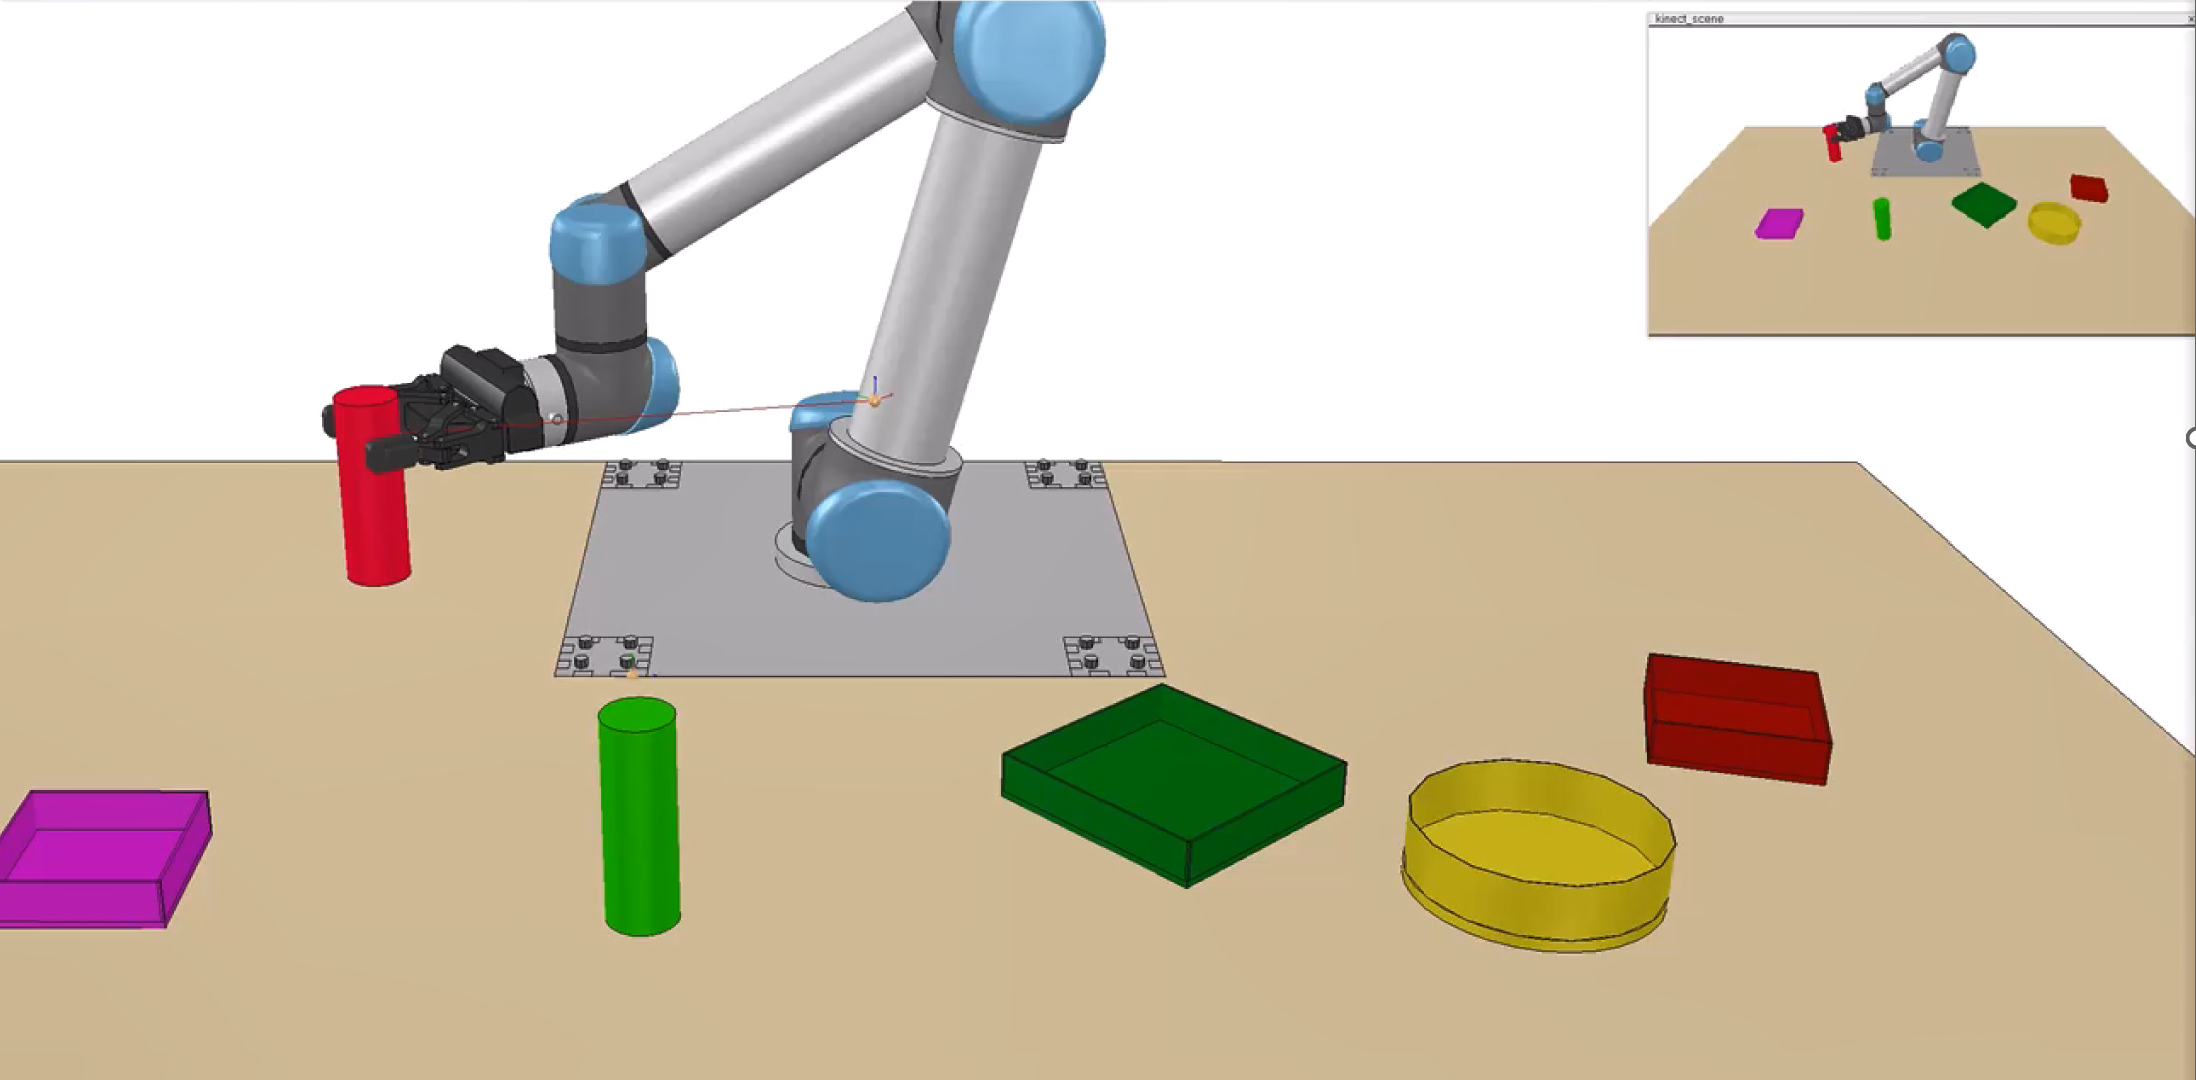
\includegraphics[width=\textwidth]{images/Language_Conditioned_Exp/theirs_1.png}
        \caption{Time step 60.}
    \end{subfigure}
    \begin{subfigure}[t]{0.18\textwidth}
        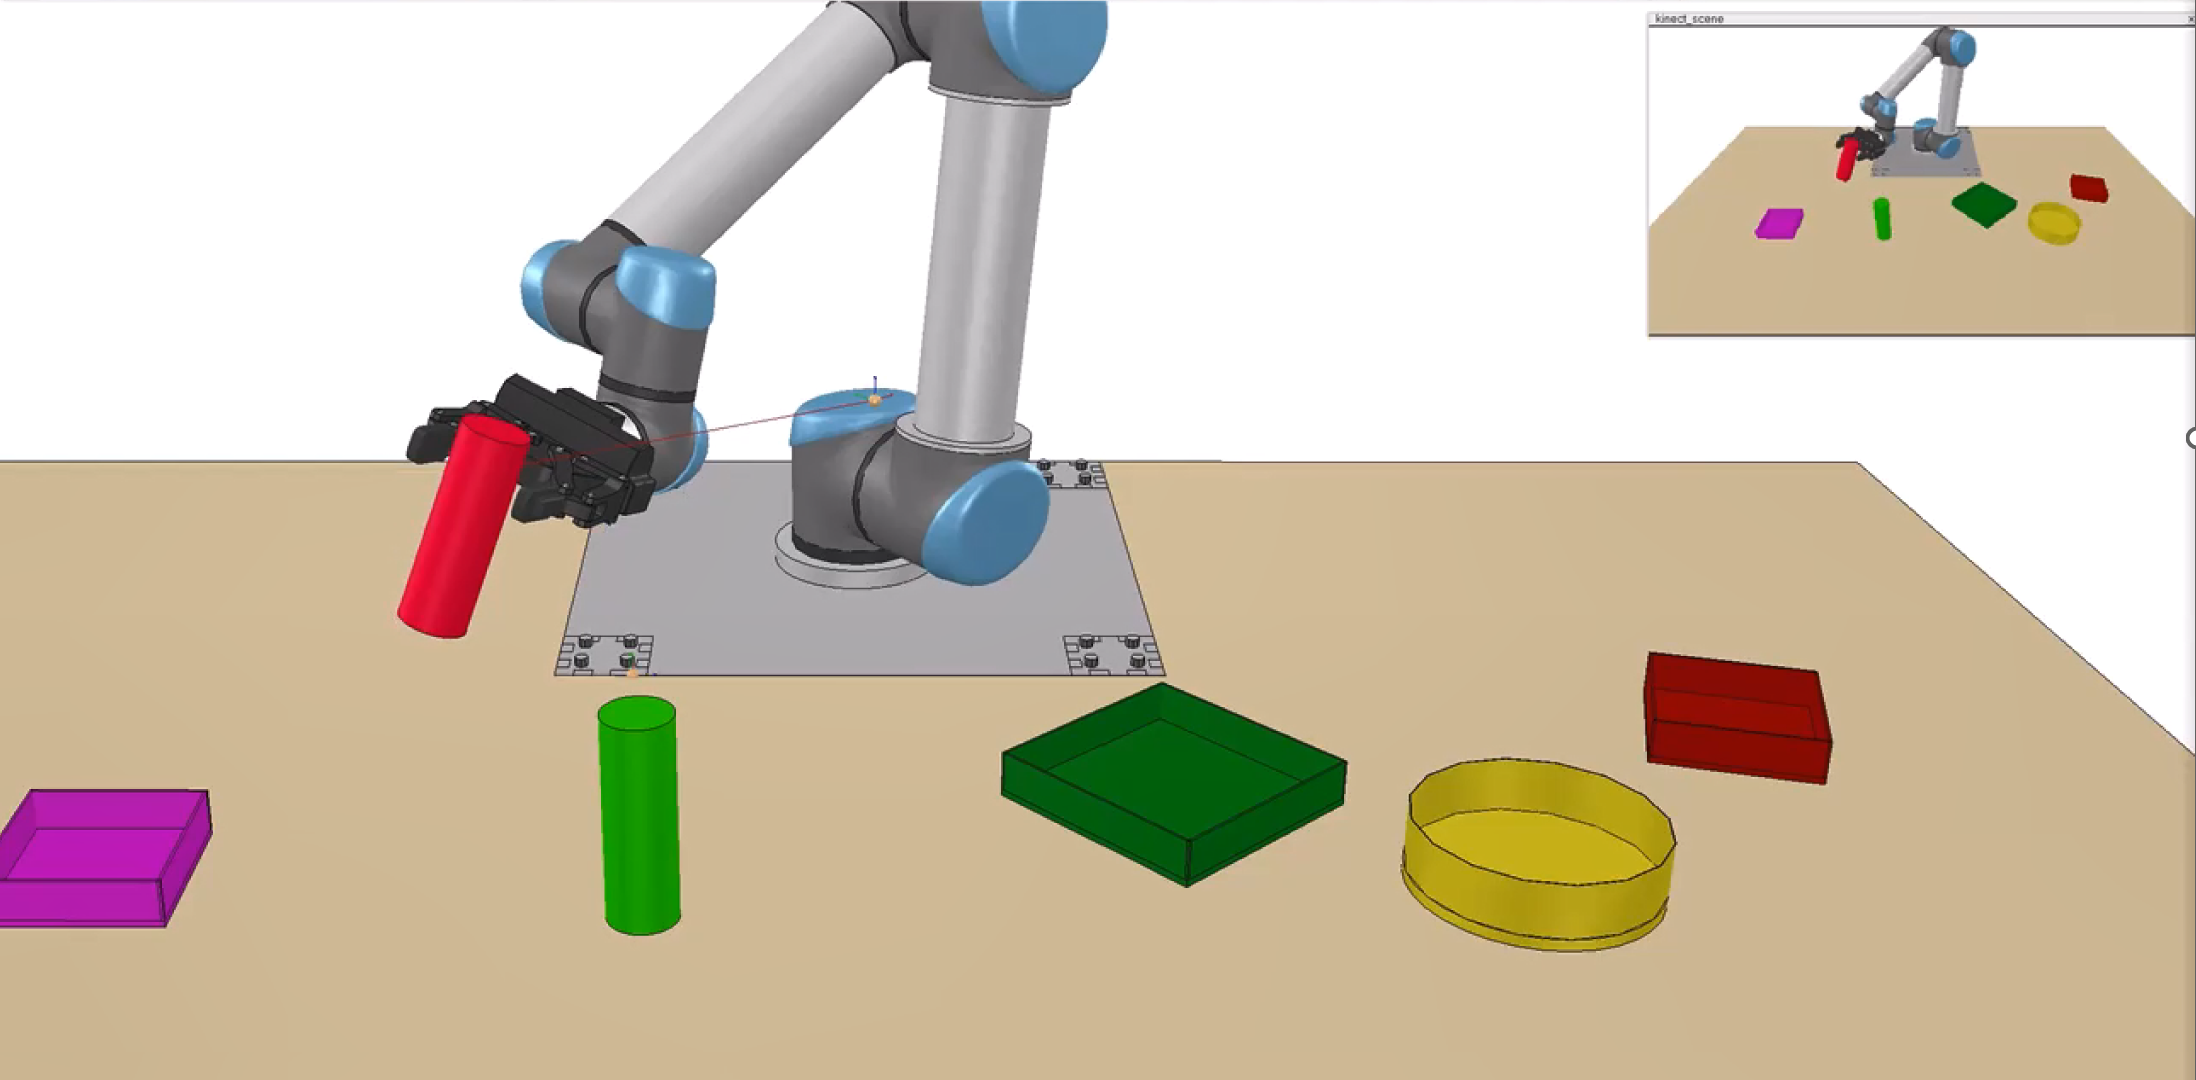
\includegraphics[width=\linewidth]{images/Language_Conditioned_Exp/theirs_2.png}
        \caption{Time step 120.}
    \end{subfigure}
    \begin{subfigure}[t]{0.18\textwidth}
        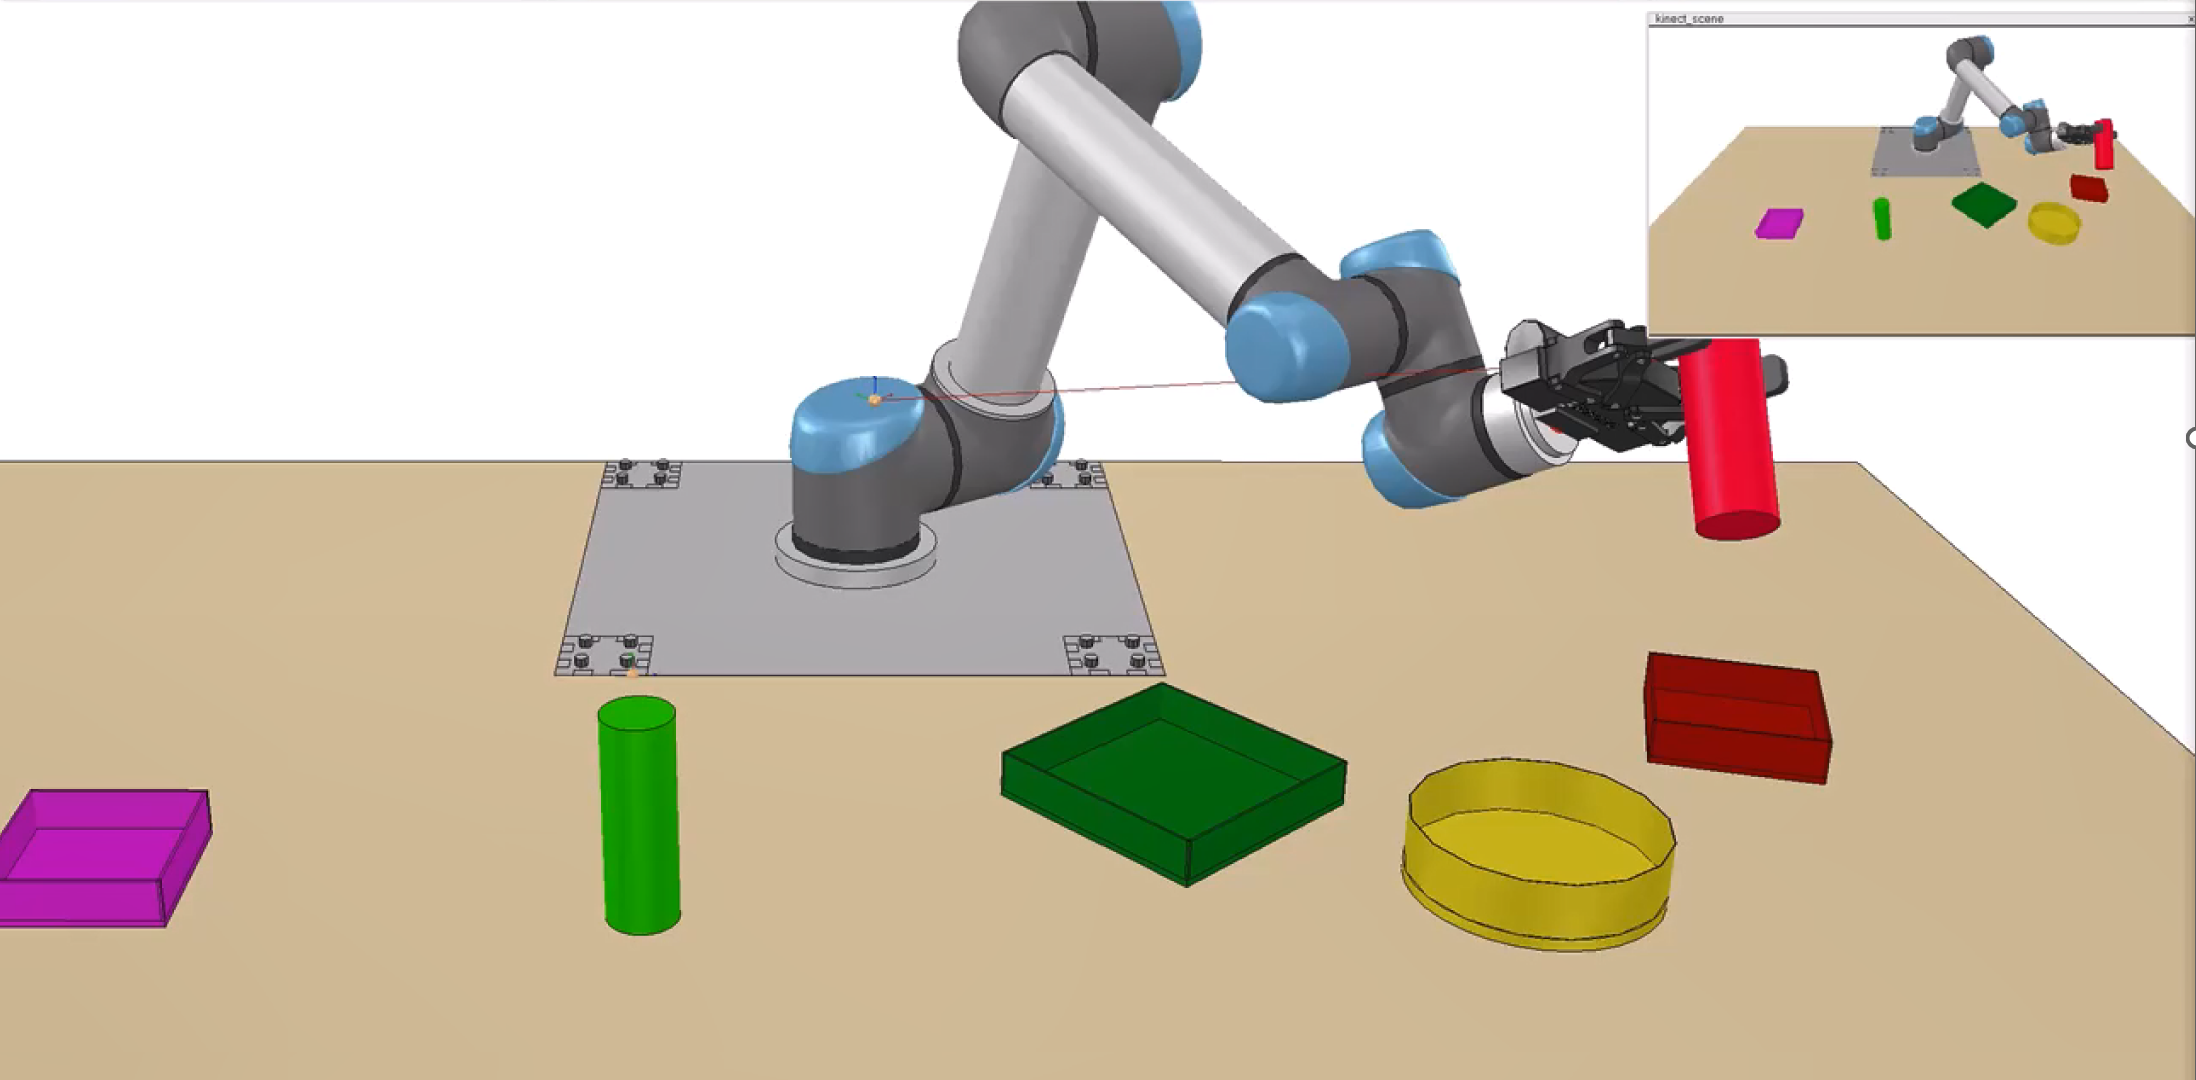
\includegraphics[width=\linewidth]{images/Language_Conditioned_Exp/theirs_3.png}
        \caption{Time step 180.}
    \end{subfigure}
    \begin{subfigure}[t]{0.18\textwidth}
        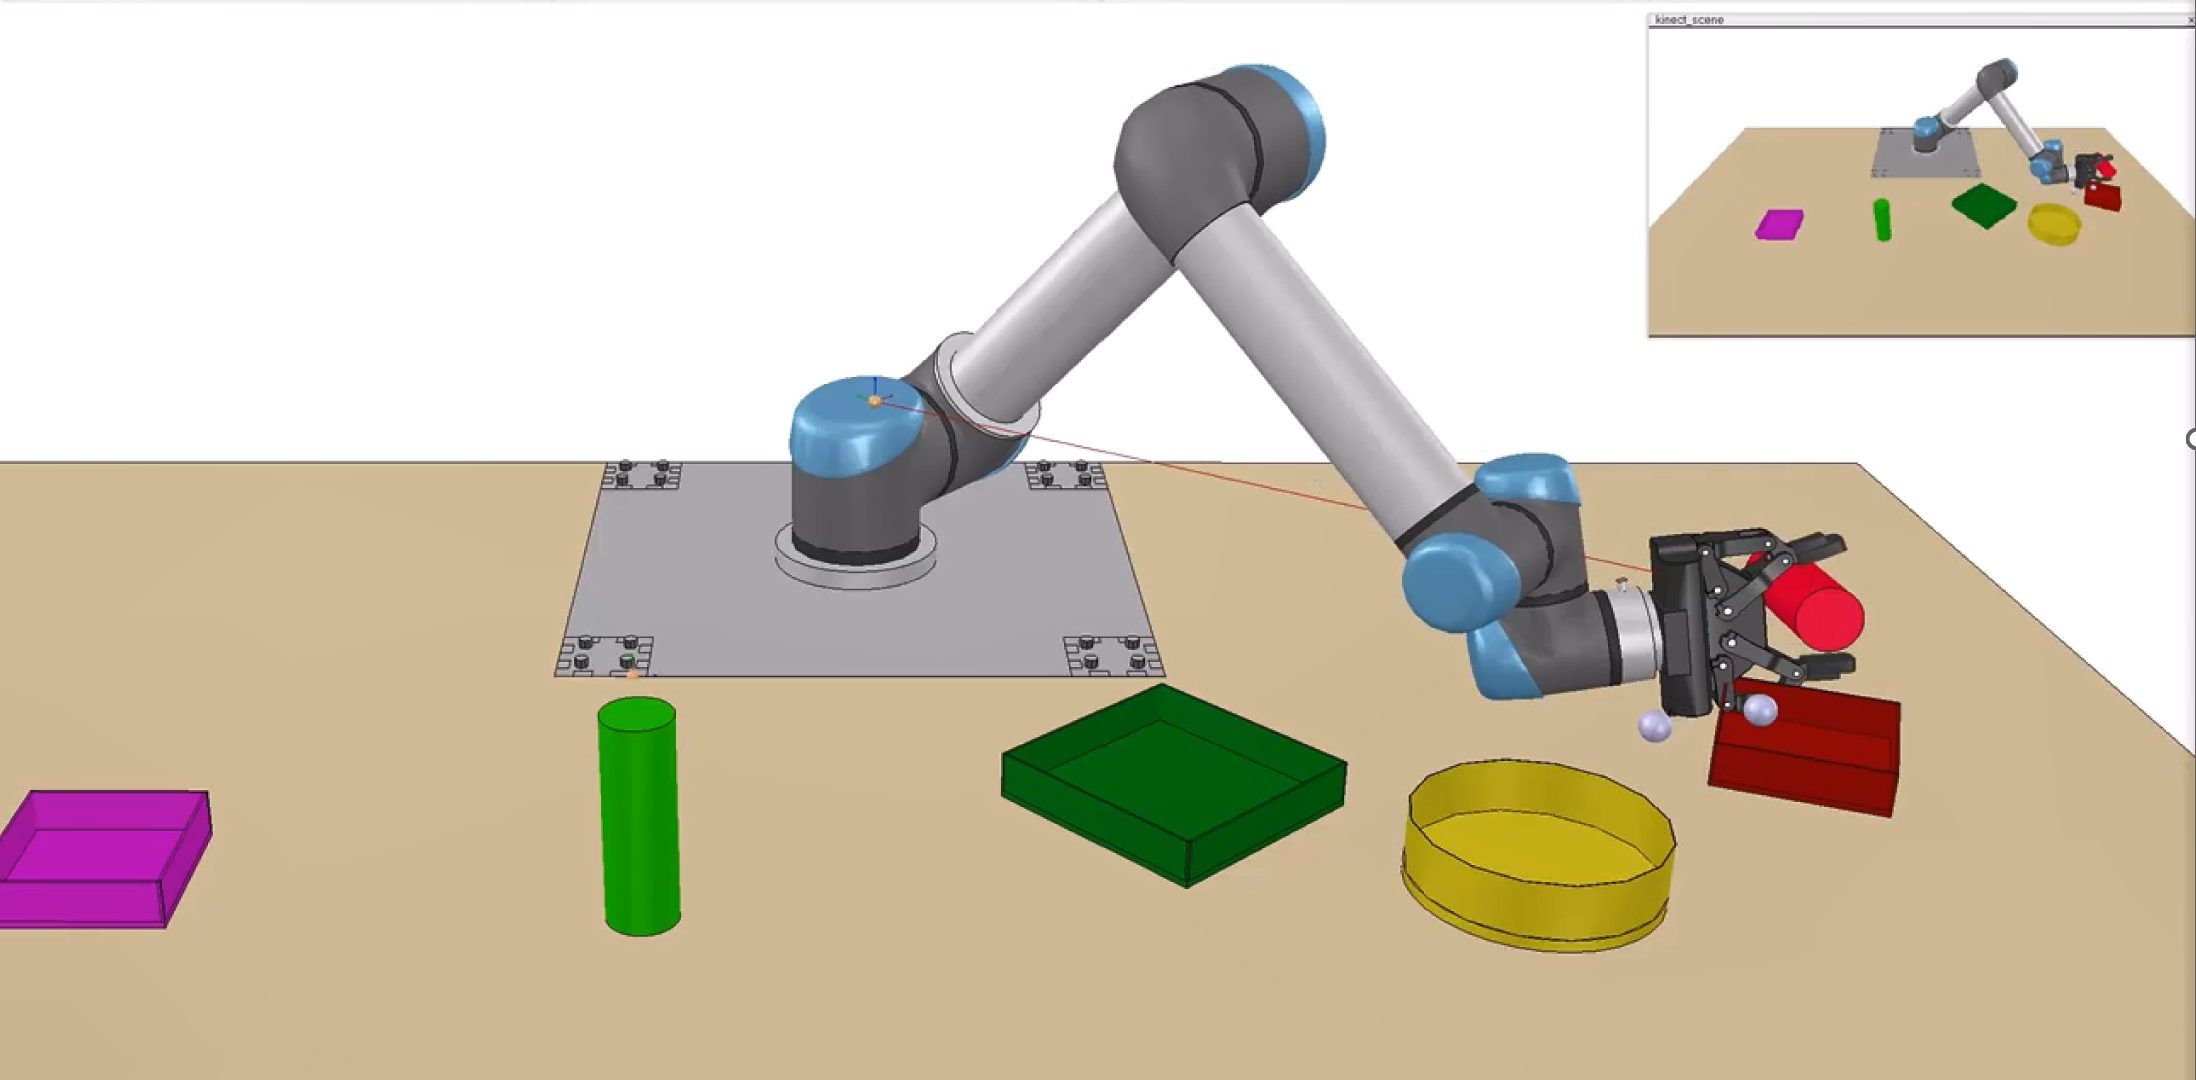
\includegraphics[width=\linewidth]{images/Language_Conditioned_Exp/theirs_4.png}
        \caption{Time step 240.}
    \end{subfigure}
    \begin{subfigure}[t]{0.18\textwidth}
        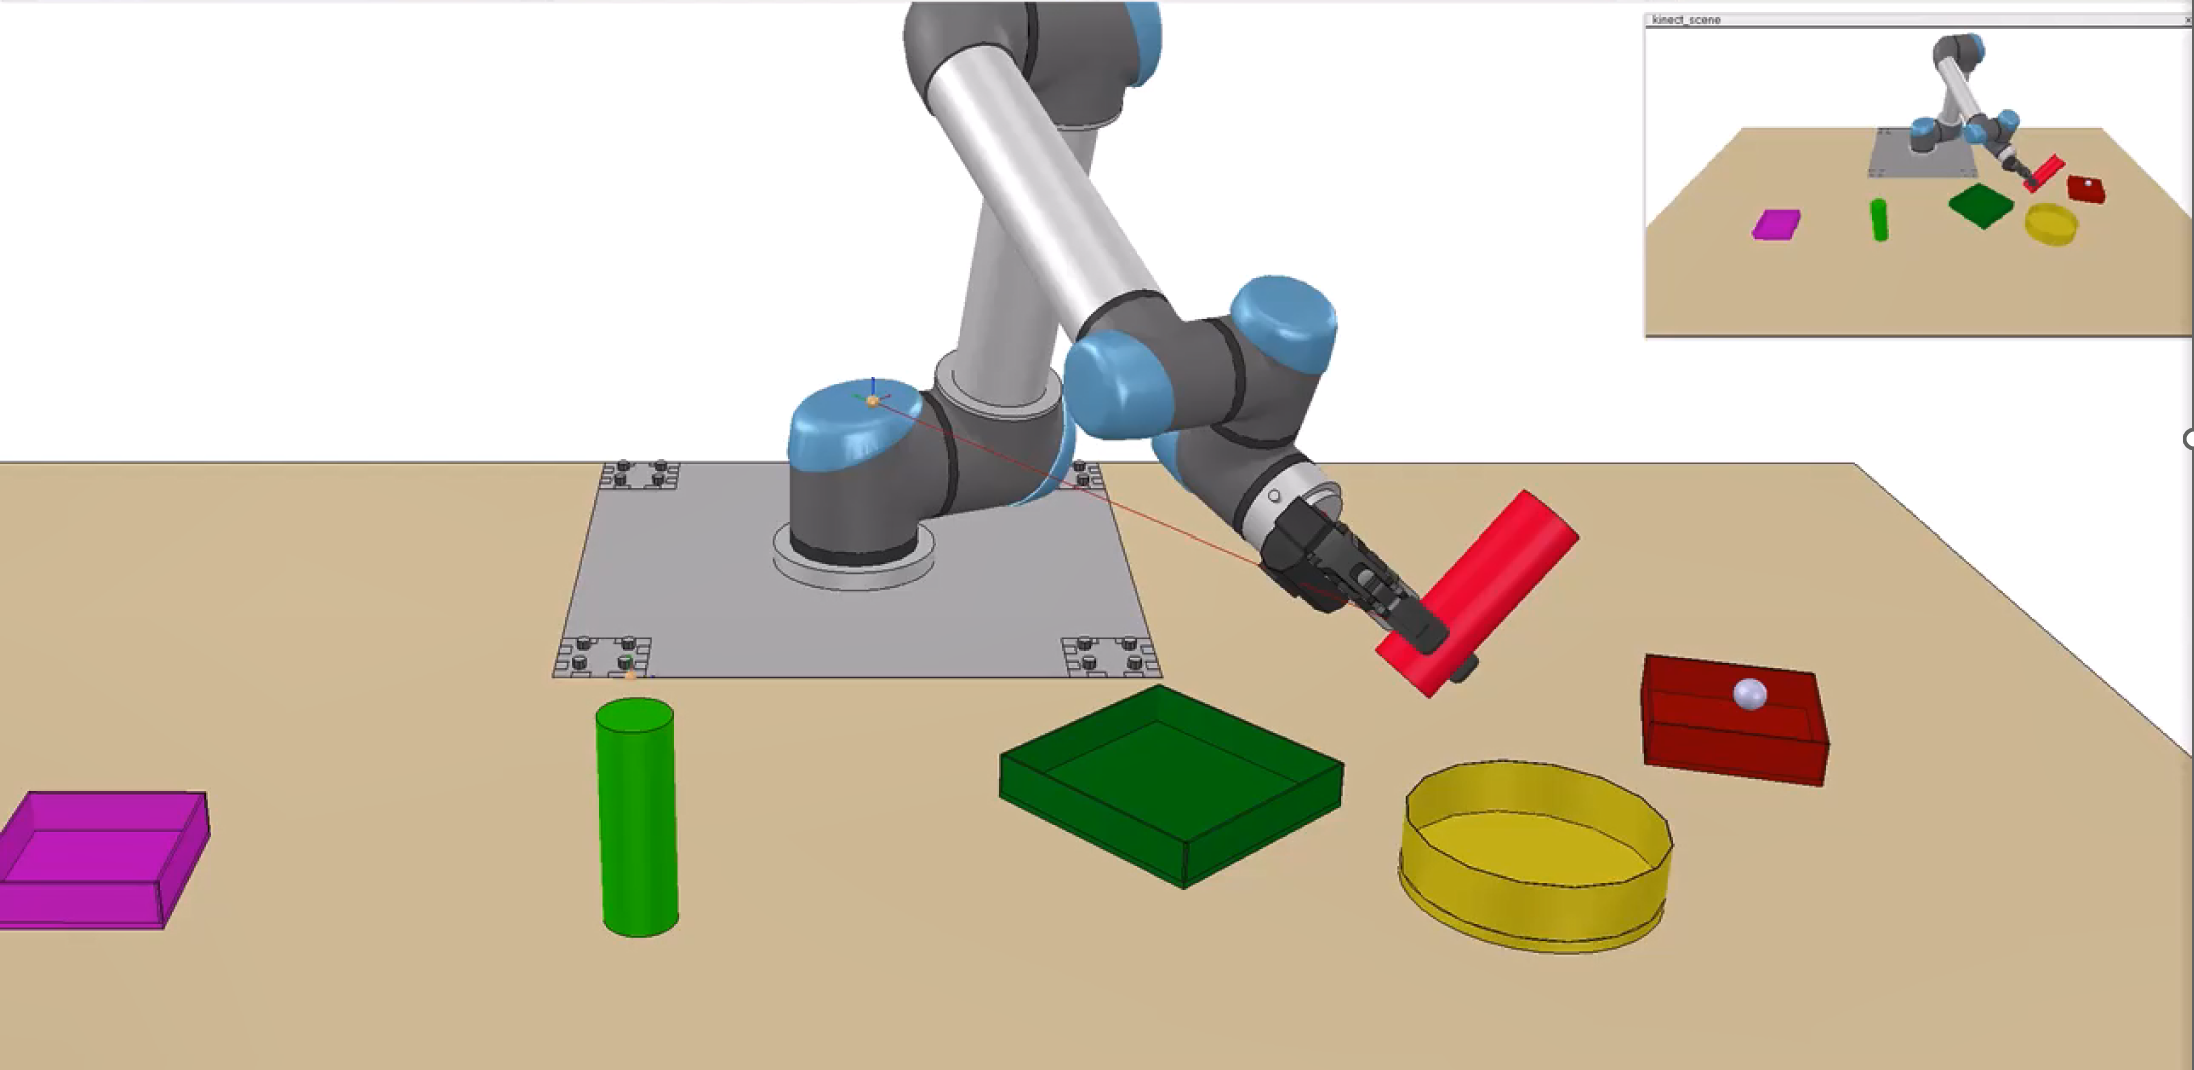
\includegraphics[width=\linewidth]{images/Language_Conditioned_Exp/theirs_5.png}
        \caption{Time step 300.}
    \end{subfigure}

    \bigskip % more vertical separation
    \begin{subfigure}[t]{0.18\textwidth}
        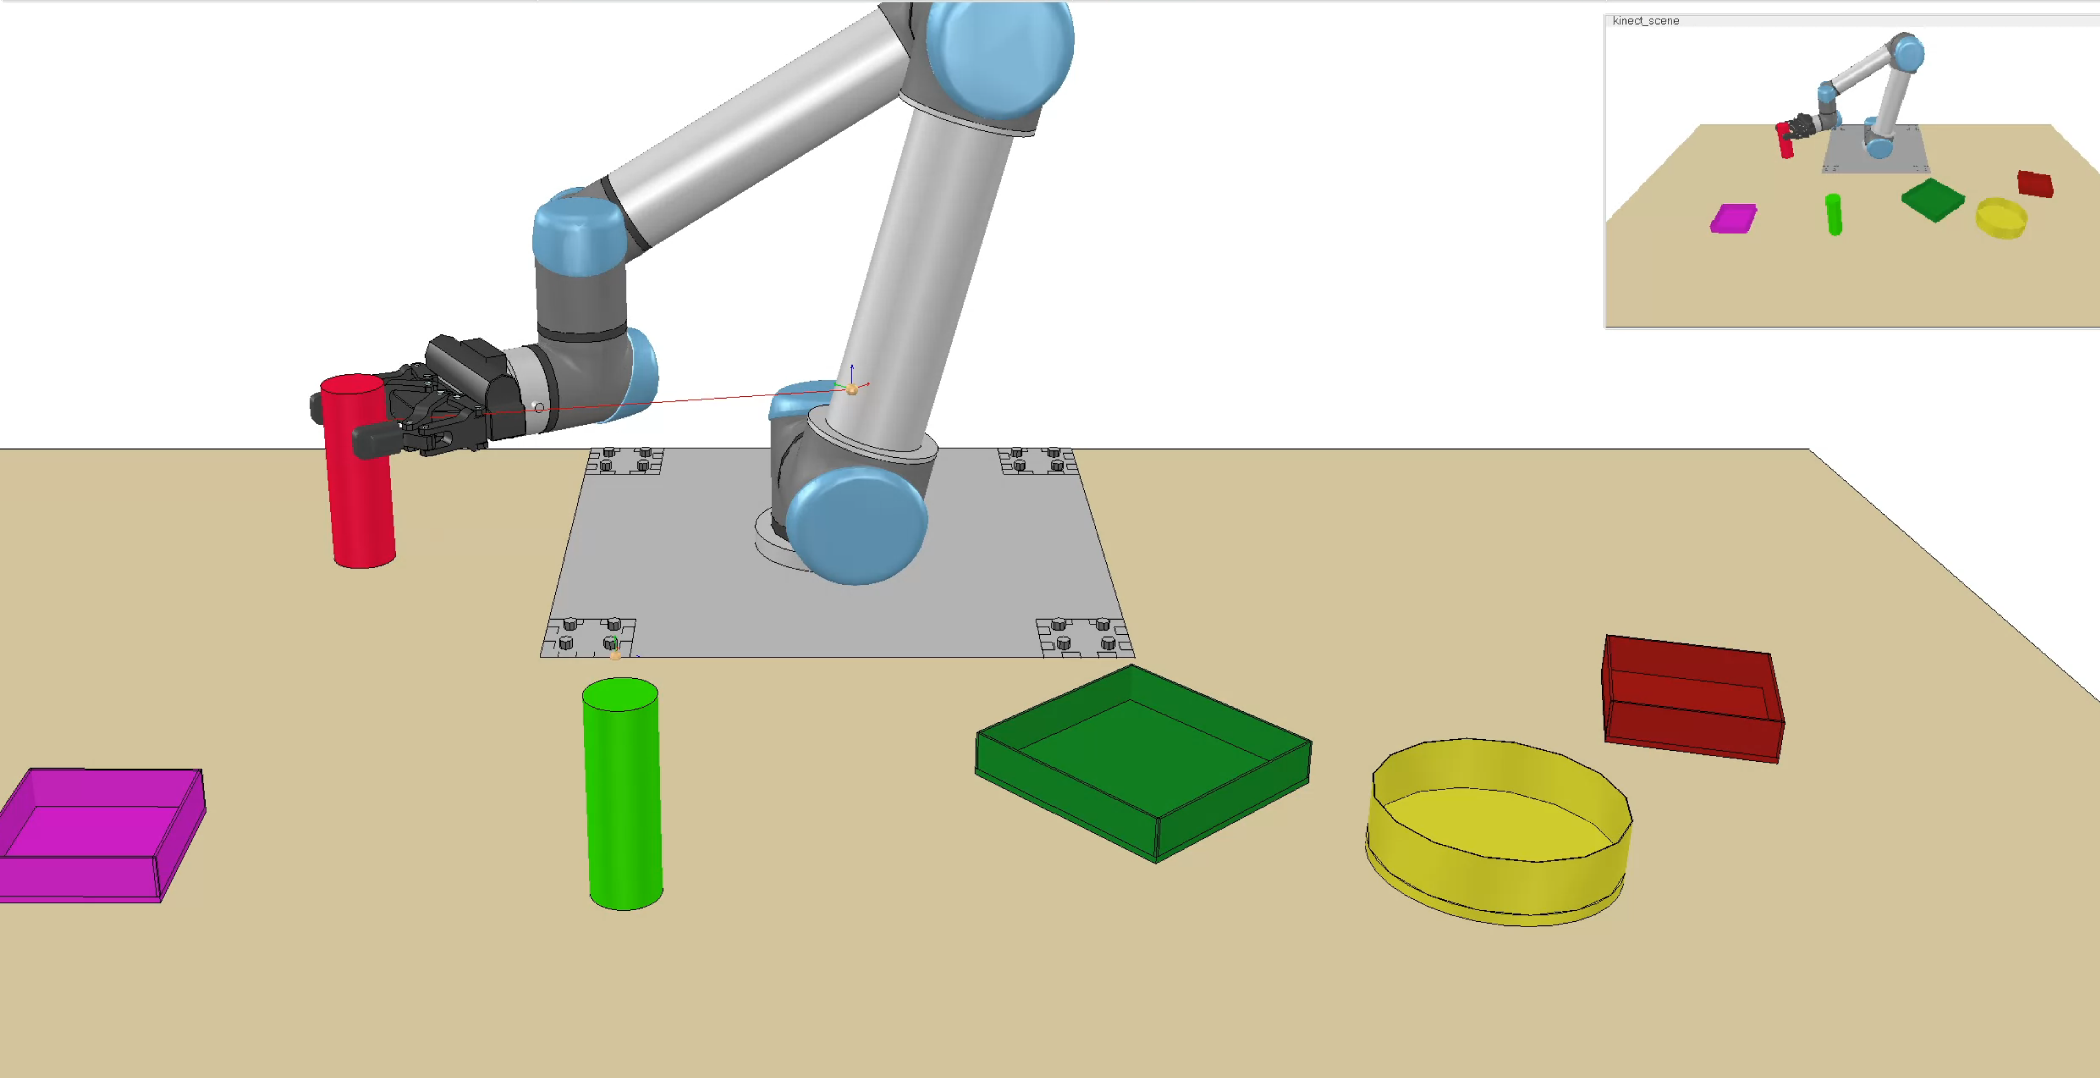
\includegraphics[width=\linewidth]{images/Language_Conditioned_Exp/mine_1.png}
        \caption{Time step 60.}
    \end{subfigure}
    \begin{subfigure}[t]{0.18\textwidth}
        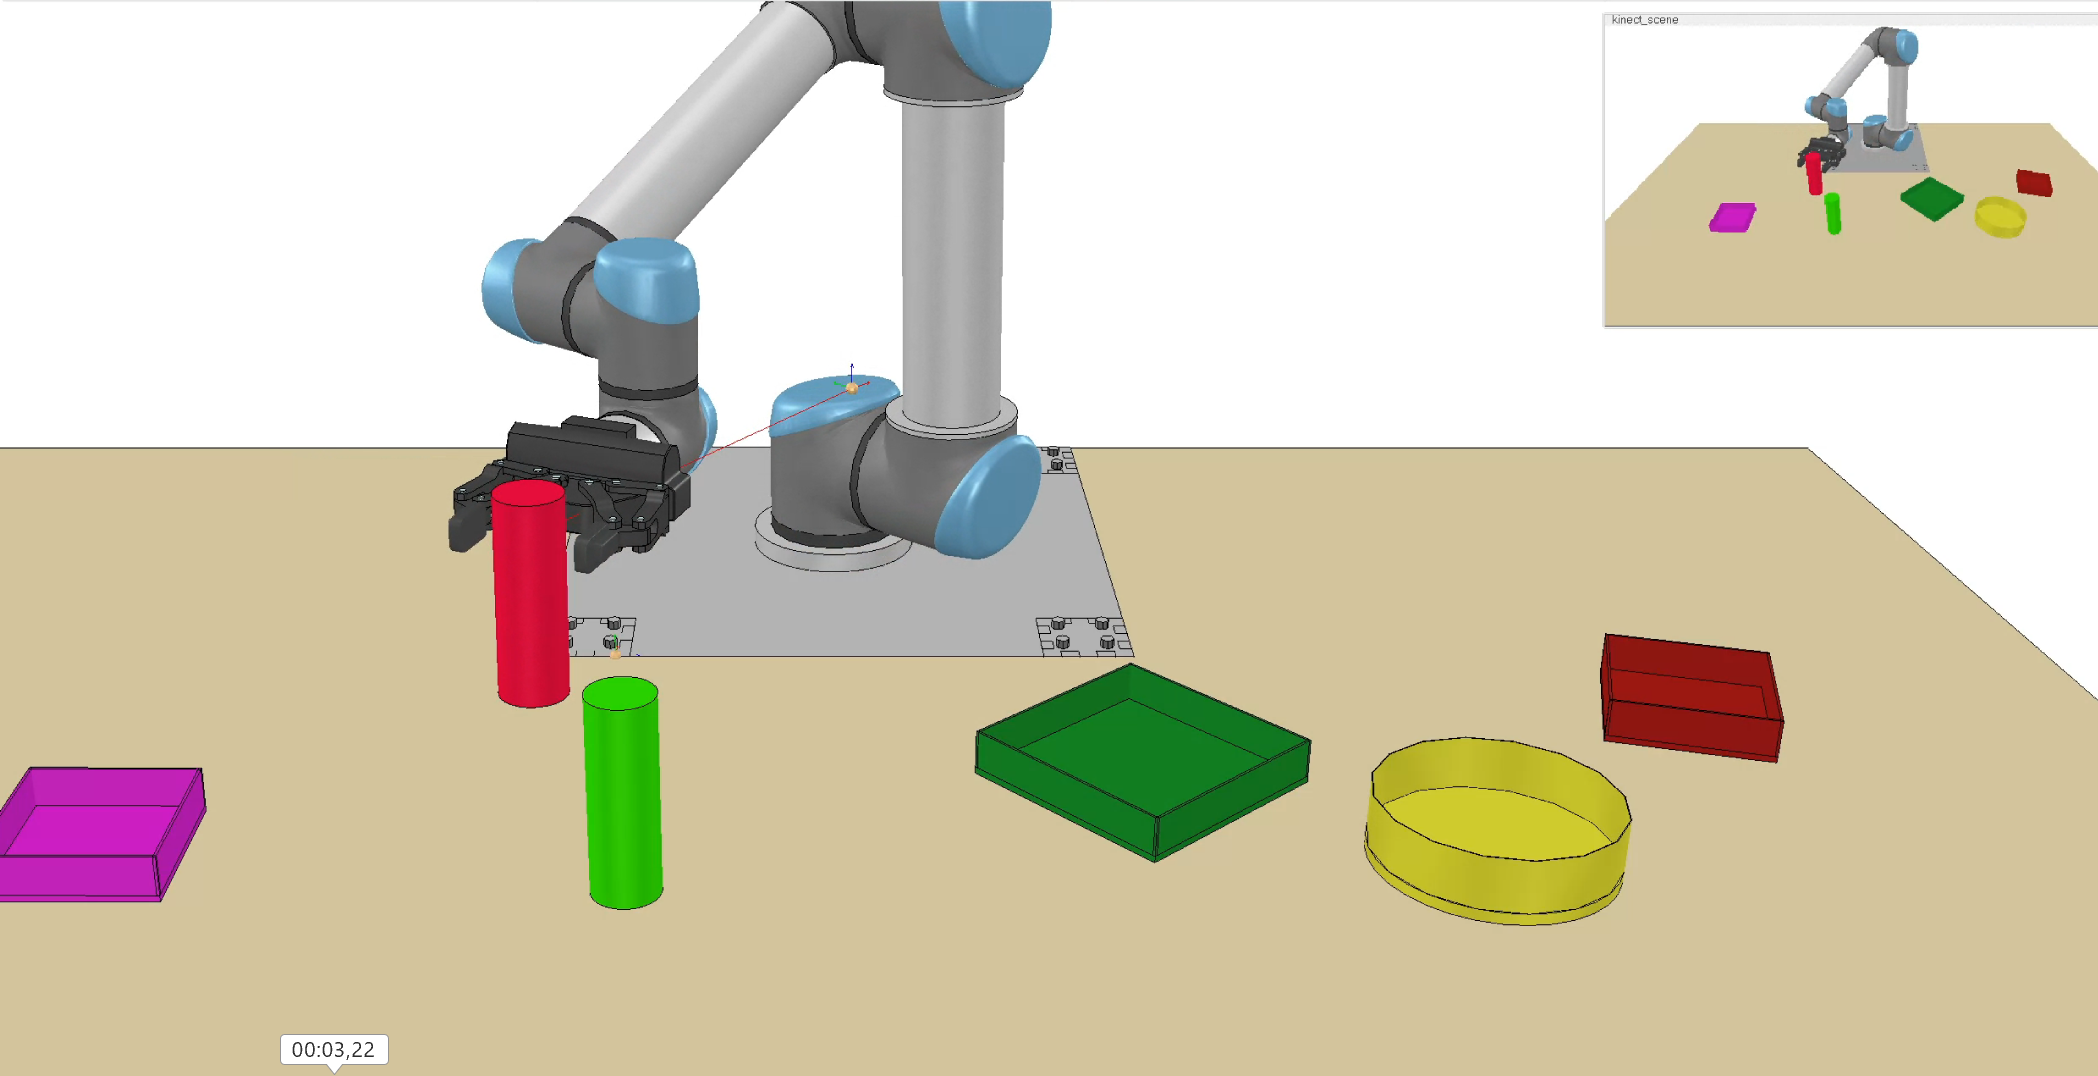
\includegraphics[width=\linewidth]{images/Language_Conditioned_Exp/mine_2.png}
        \caption{Time step 120.}
    \end{subfigure}
    \begin{subfigure}[t]{0.18\textwidth}
        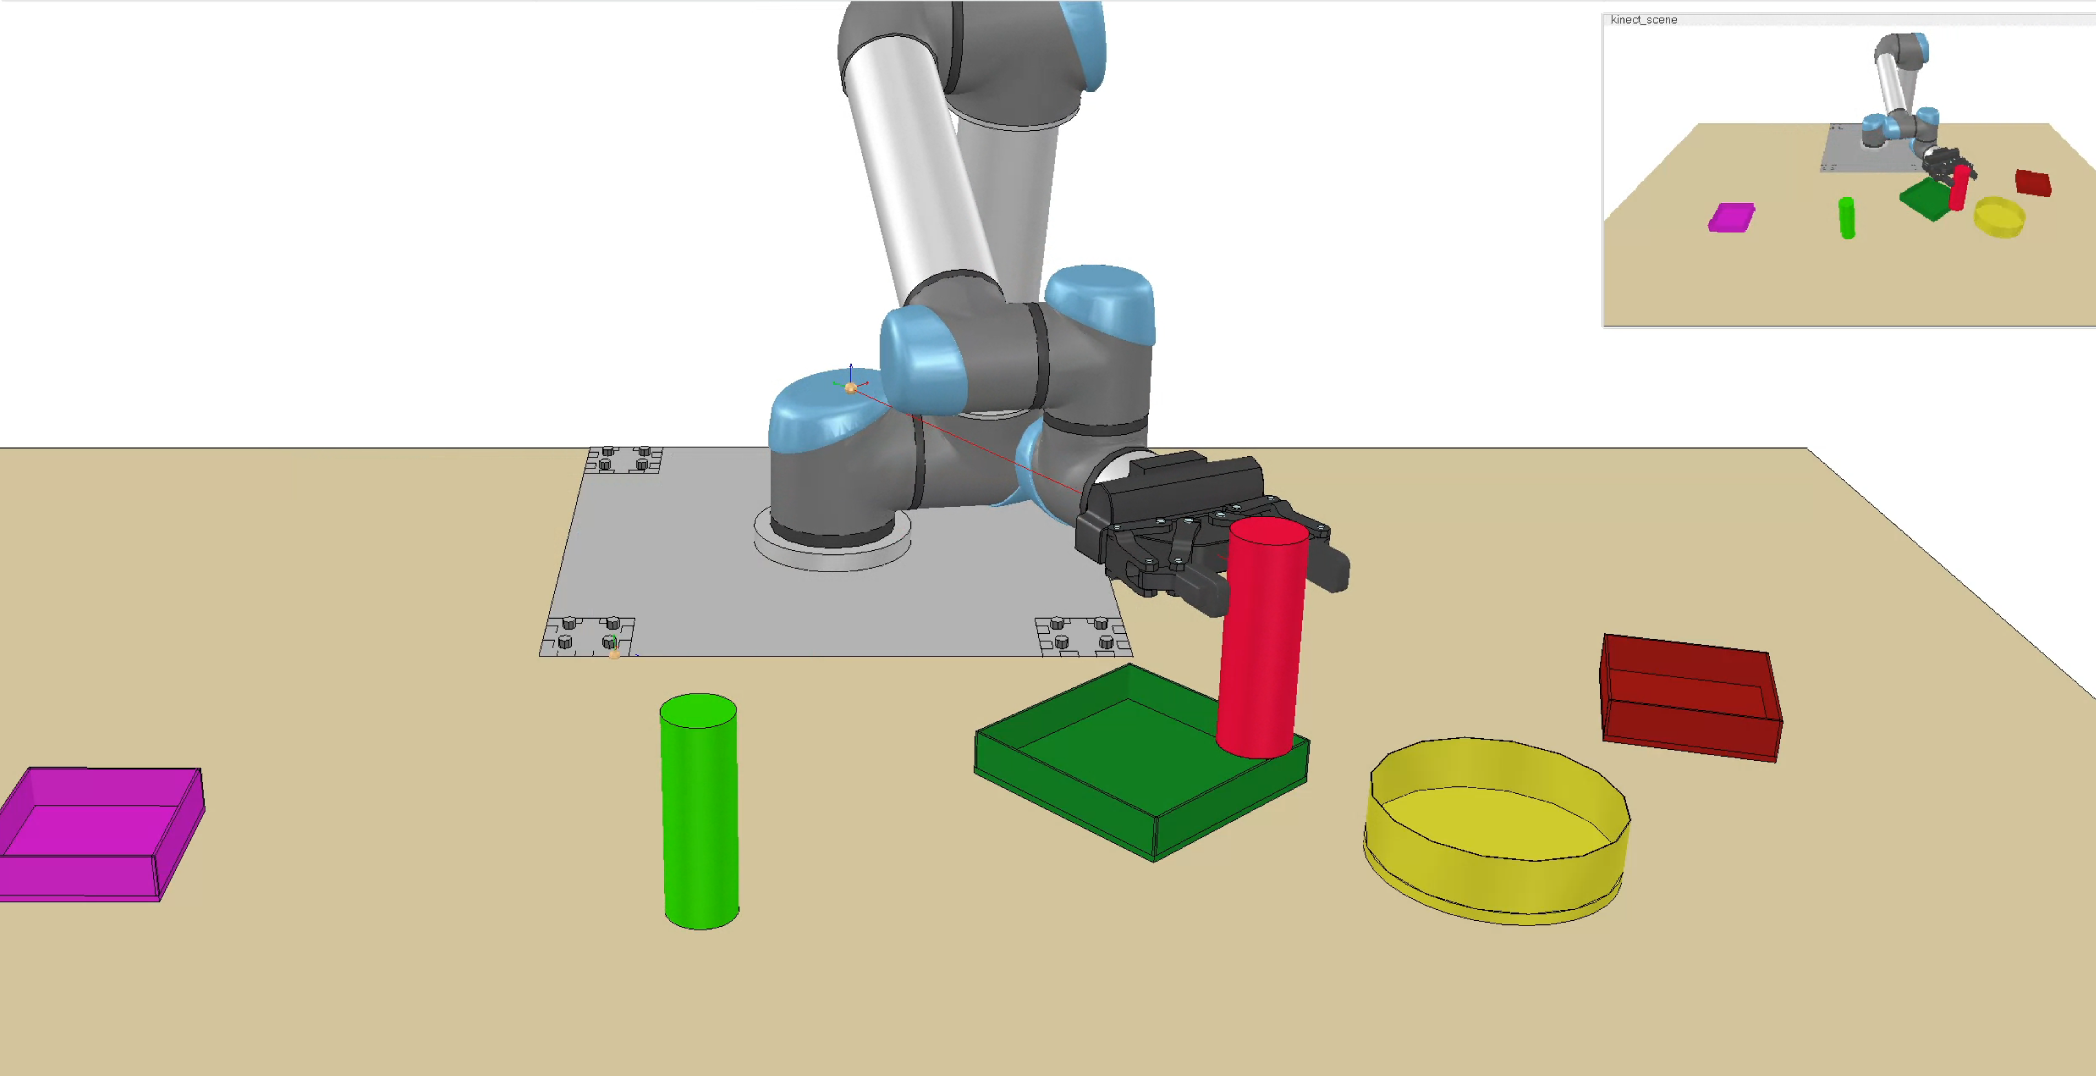
\includegraphics[width=\linewidth]{images/Language_Conditioned_Exp/mine_3.png}
        \caption{Time step 180.}
    \end{subfigure}
    \begin{subfigure}[t]{0.18\textwidth}
        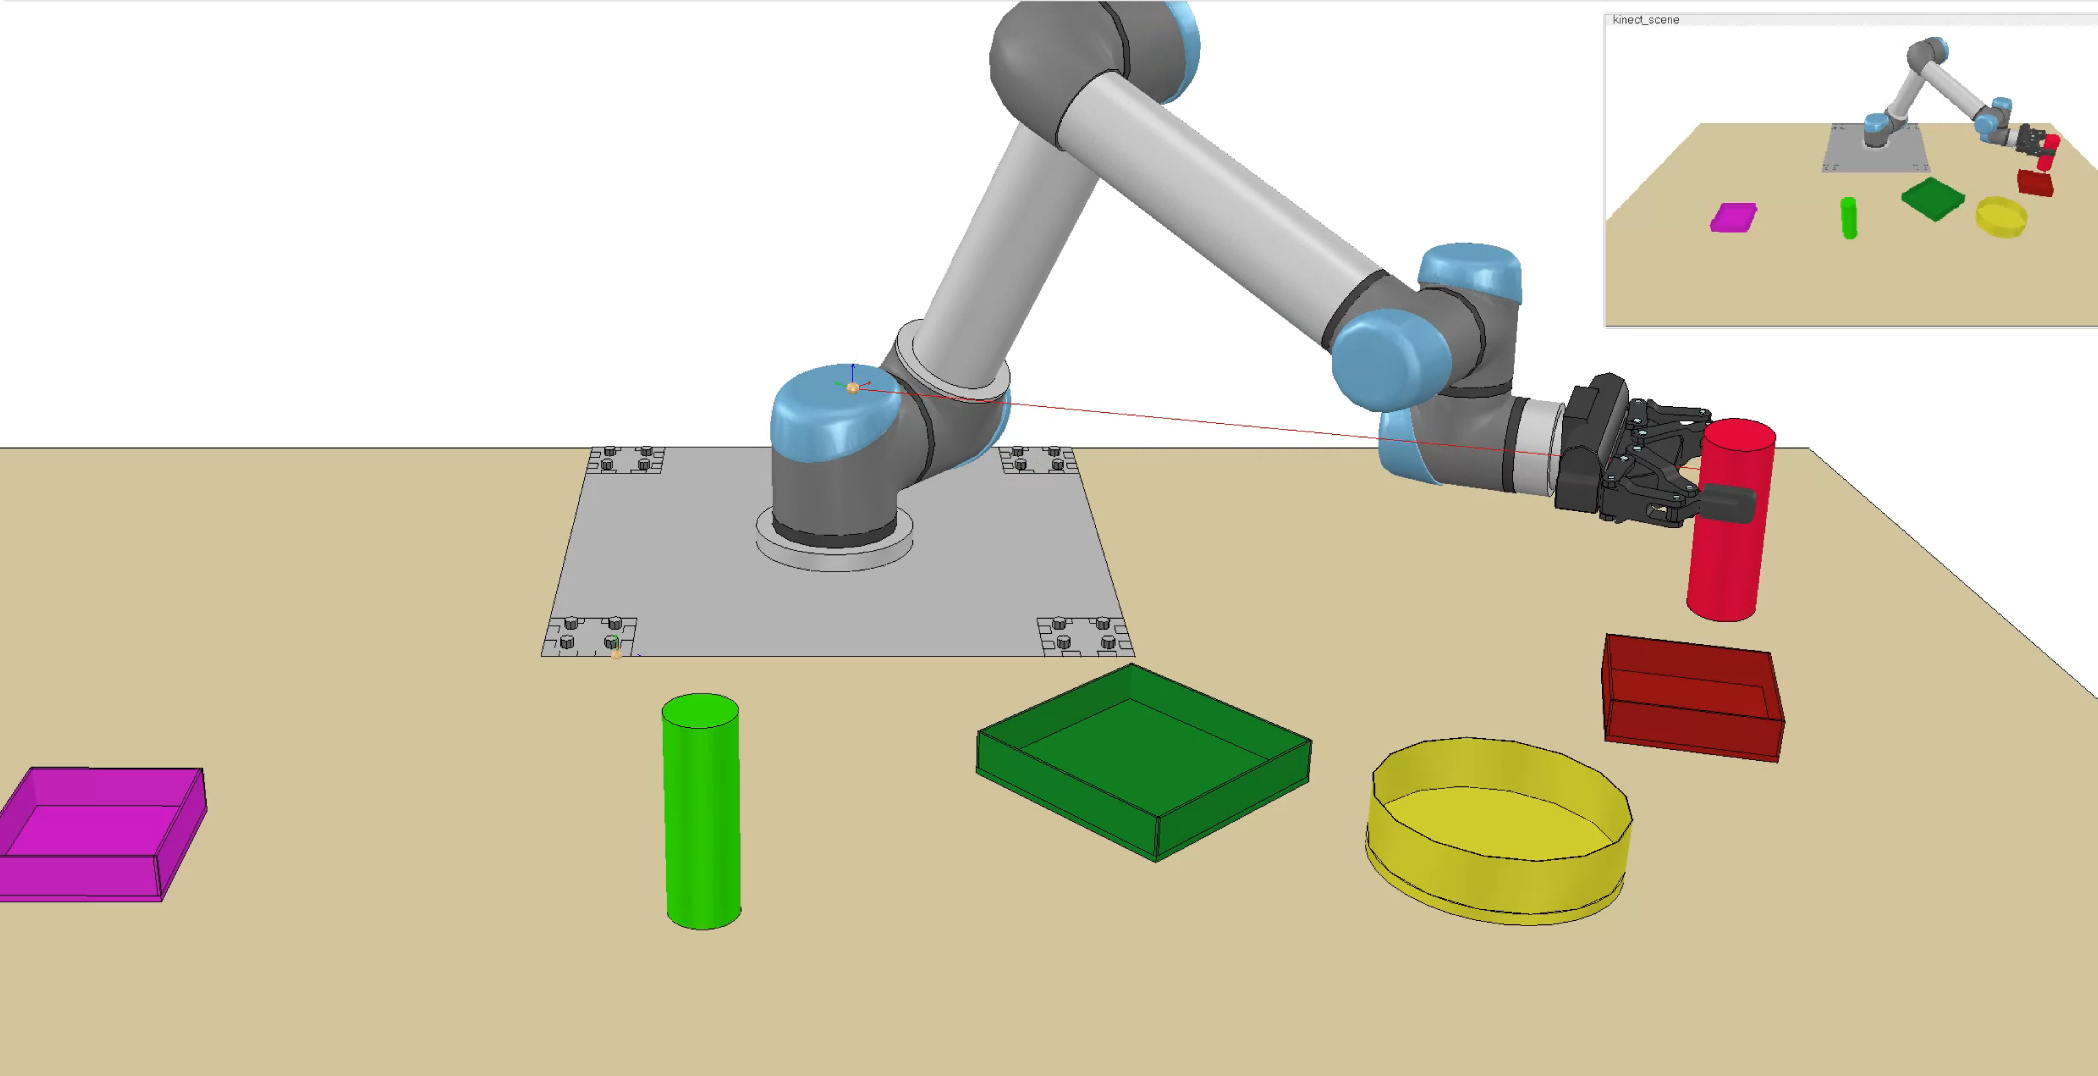
\includegraphics[width=\linewidth]{images/Language_Conditioned_Exp/mine_4.png}
        \caption{Time step 240.}
    \end{subfigure}
    \begin{subfigure}[t]{0.18\textwidth}
        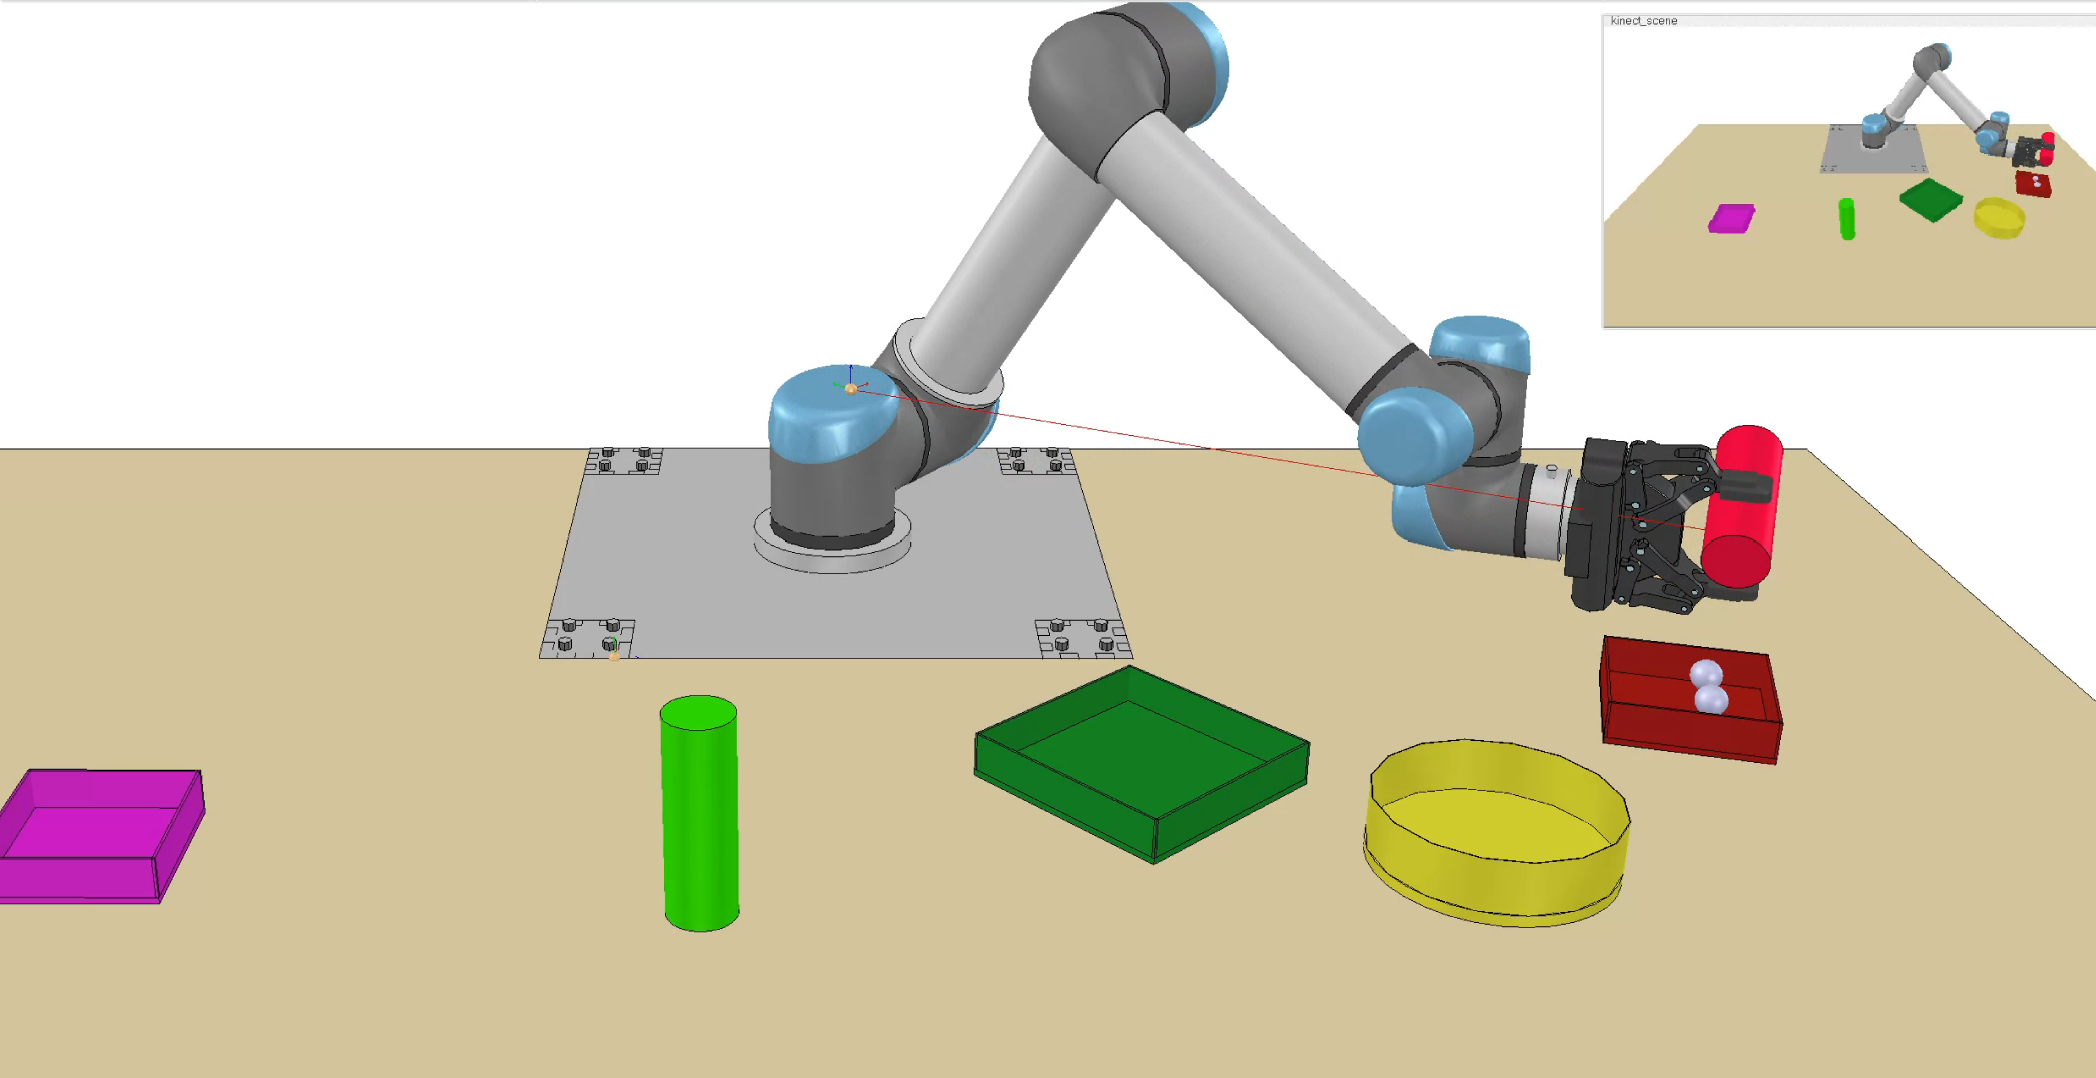
\includegraphics[width=\linewidth]{images/Language_Conditioned_Exp/mine_5.png}
        \caption{Time step 300.}
    \end{subfigure}
    \caption{Comparison of a pour task. The policy learned by the LCIL algorithm (top row) spills the content over the table and moves unpredictable. The task is considered a failure 
    by the benchmark, as most drops did not land in the goal bowl. Active critic (bottom row) performs the task as intended with no unexpected movement.}
    \label{fig: AVC vs. Rec}
\end{figure}
Furthermore, in Figure \ref{fig: AVC vs. Rec}, we have depicted a case in the test dataset that our policy solved and compared it to the performance 
of the recurrent algorithm, which failed at the task.
While our approach hit the target precisely, the recurrent model was widely off. We assume that this is caused by the fact that during inference 
time, the
i.i.d. assumption of the input data to the policy is broken. Intuitively, the recurrent policy
is in a state that it has not seen before and acts slightly differently to the expert movement. After some steps, the policy now sees 
inputs that are vastly
different from the training distribution, thus it starts to act unpredictably. As argued in Section \ref{COD_AC}, this is an advantage of our 
policy as it
does not break the i.i.d. assumption.

\section{Reinforcement Learning from Sparse Rewards in Single Observation Environments}
In this section, we will explore the performance of the AVC algorithm given a single observation per trajectory, one sparse reward per trajectory, and some expert demonstrations.
We motivated the practical relevance in the introduction. An additional advantage for testing the effectiveness of the search paradigm is that planning is most efficient in
single observation settings.
We discussed this in section \ref{sec:AC_Critic}, where we state that while predicting the MDP has a quadratic error bound, we don't get any updated information
during the trajectory, and thus no better estimate is possible. \\

We chose environments from the "Meta-World" \ref{yu2019meta} benchmark, as they have a success indication per environment, from which sparse rewards can be defined naturally.
Specifically, we chose five environments from the ML10 suite, namely "Pick and Place", "Push", "Reach", "Window Open" and "Drawer Close", which represent a variety
of difficulty levels suited to test different aspects of our algorithm. We defined a constant sequence length of 100 steps per trajectory and provided
a reward at the end according to whether the environment was solved at any step along the trajectory. Additionally, the environment
only returns the initial observation along the trajectory.\\

The single observation setup is not well-studied in continuous spaces, so we have to find baselines that are best suited to challenge the performance of our algorithm. For sparse rewards, a common
algorithm is "HER" as discussed in section \ref{sec:HER}, but it assumes a way to compute the goal from an environment state. This is not suitable in our setup, as we don't have access to the environment
states after the first state. Moreover, this assumption limits the generality of the approach, which AVC does not need to.
We use PPO, a state-of-the-art on-policy algorithm, and TQC, a state-of-the-art off-policy algorithm, together with transformer-style sequential encoding to indicate the timestep. We also include
RPPO, a recurrent implementation of PPO, where we repeatedly input the initial observation and use the hidden states to encode the position along the action sequence.
PPO, TQC, and RPPO were pre-trained using behavioural cloning. We chose the best-performing policy during behavioural cloning by testing the policy on 50 test
trajectories every 400 full cycles through the
expert transitions. Technically, these test trajectories were environment interactions, but we chose not to count them to give the best-case comparison to the AVC algorithm, which was not pre-trained.\

For the base implementations, we use "Stable Baselines3" \ref{stable-baselines3}, which is a common choice, as it provides well-implemented algorithms with tested
performance and fine-tuned hyperparameters for a wide range of environments. This includes our chosen environments, but with dense rewards and continuous observations,
thus some hyperparameter tuning was necessary. \\

In the following sections, we will test our algorithm in two different settings, namely fine-tuning and guided reinforcement learning. In fine-tuning, we provide
enough expert demonstrations, that the environment can be solved with acceptable performance, but with room for improvement. In guided reinforcement learning,
only one expert demonstration is provided. AVC will use the same set of hyperparameters for all experiments to showcase its generality and robustness. Also, we had no choice for time constraints.
We will use limited fine-tuning for the baselines, however.
With these experiments, we aim to test both exploitation and exploration of our algorithm and show stable
behaviour across a wide range of use cases. \\

In all plots, the first data point is sampled from the policy before any environment interaction. For the plots with behavioural cloning, it indicates learned performance from expert trajectories.
In plots with no provided expert trajectory, it displays the behaviour following random initialisation.


\subsection{Fine Tuning}
\label{sec:fine_tuning}
In this section, we analyse our algorithm in a fine-tuning setup. We provided the algorithms with 4 and 15 expert demonstrations per 
environment and used a relatively short reinforcement learning phase with 400 sampled trajectories consisting of 100 steps each. We 
repeated each experiment four times with 30 test trajectories per datapoint. One problem we wanted to overcome is "catastrophic forgetting" 
that can occur when the data distribution shifts. During the imitation phase, the learners only see positive examples sampled according to 
the distribution induced by the expert, which leads to overestimation by the critic. Our algorithm is more robust to this problem, as it 
decouples the actor from the critic, as discussed in section \ref{inference_time_planning}. We present our findings in figure \ref{fig:finetuning}. 
For the environments "Pick and Place" and "Push", we show the plots for 15 expert demonstrations, as we found 4 expert demonstrations were not 
enough to meaningfully learn within 400 training episodes. The environments "Reach" and "Window Open" are easier to learn, so we display the 
experiments with 4 expert demonstrations each, as giving 15 expert demonstrations lead to near perfect performance from imitation learning alone. 
All plots for all experiments can be found in Appendix \ref{chapter:additional_plots}.\\

We expected RPPO to be the least performant from our discussion of the curse of dimensionality in section \ref{COD_AC}. As no current input 
is provided from the environment, RPPO has to keep track of all previous actions. PPO and TQC use positional encoding to indicate the current 
timestep which makes the problem easier. The algorithms guided by GAIL did not improve meaningfully. We assume the limited amount of environment 
interaction was not proficient to learn a good discriminator and improve the policies. We found that the performance of the baselines was most 
reliant on the learning rate. Too high values lead to catastrophic forgetting. The values we chose were the highest possible values before 
catastrophic forgetting took place. However, the performance from behavioural cloning, indicated by the first datapoint per plot, was mostly 
the best achievable performance. PPO tends to do better than TQC in the single observation setup in general. We expect this is due to the 
fact that TQC's strength as an off-policy algorithm lies in exploration. In our chosen setup, exploration is specifically hard, given no 
information from the environment during the trajectories.\\

We find that AVC is the only algorithm that can meaningfully improve its performance given the limited amount of environment interactions. 
We propose this is due to the fact that catastrophic forgetting is not a problem with AVC, as discussed earlier in this section, which makes 
it specifically suitable for fine-tuning.

\begin{figure}[htbp]
    \centering
    \begin{subfigure}[t]{0.45\textwidth}
      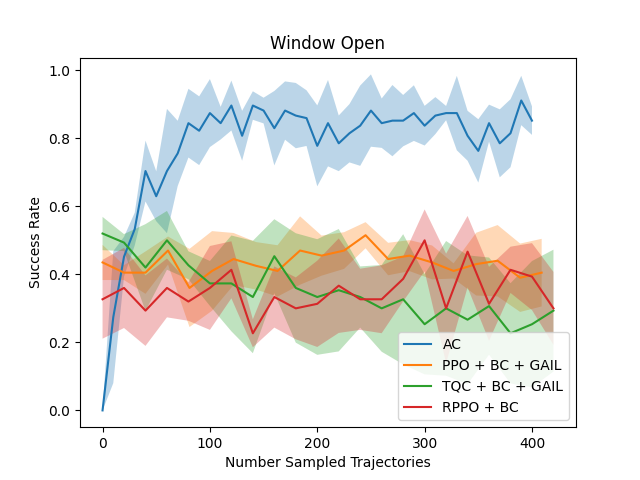
\includegraphics[width=\textwidth]{images/FineTuning/Window Open.png}
      \caption{Window Open environment, 4 expert demonstrations.}
      \label{fig:plot3}
    \end{subfigure}
    \begin{subfigure}[t]{0.45\textwidth}
      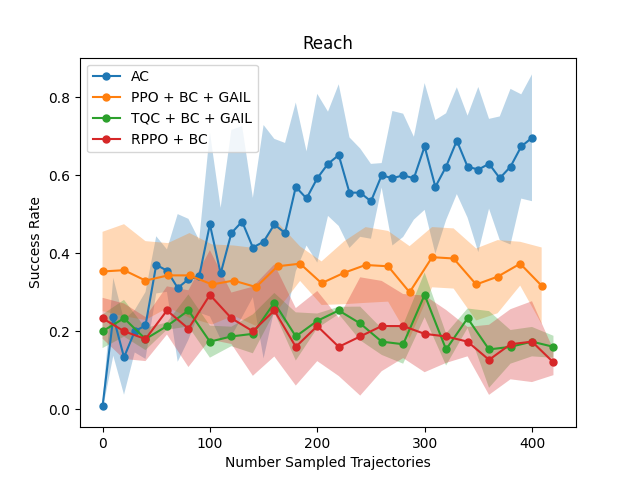
\includegraphics[width=\textwidth]{images/FineTuning/Reach.png}
      \caption{Reach environment, 4 expert demonstrations.}
      \label{fig:plot1}
    \end{subfigure}
    \medskip
    \begin{subfigure}[t]{0.45\textwidth}
      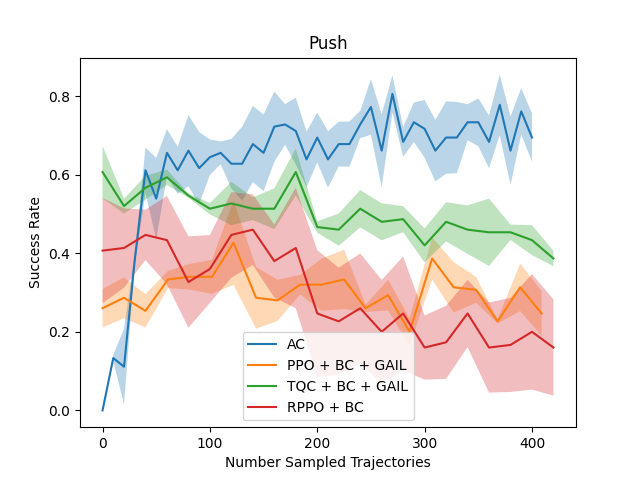
\includegraphics[width=\textwidth]{images/FineTuning/Push.png}
      \caption{Push environment, 15 expert demonstrations.}
      \label{fig:plot2}
    \end{subfigure}
    \begin{subfigure}[t]{0.45\textwidth}
      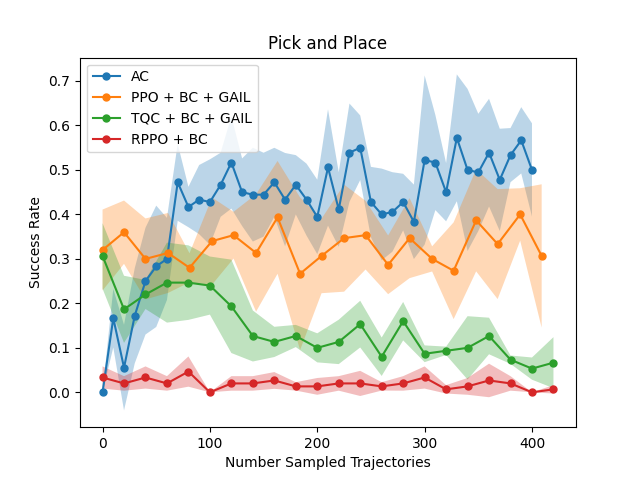
\includegraphics[width=\textwidth]{images/FineTuning/Pick and Place.png}
      \caption{Pick and Place environment, 15 expert demonstrations.}
      \label{fig:plot4}
    \end{subfigure}
    \caption{
    The learner trained by GAIL and RPPO were pretrained using behavioural cloning with the given number of expert demonstrations. 
    The x-axis shows the number of sampled environment episodes, each with 100 steps.  One initial observation and a sparse reward signal at the end of each episode was provided.}
    \label{fig:finetuning}
\end{figure}

\subsection{Guided Reinforcement Learning}
\label{sec:g_ref_ler}
In this section, we test the performance of AVC given minimal expert guidance. We use the "Reach" and "Window Open" environments with 2000 training episodes per run and three runs per experiment and learner.
Per data point, we sampled 30 trajectories to evaluate the success rate.\\
With this setting, the algorithms must learn most of the behaviour from reinforcement learning, but the expert
demonstration is needed to overcome the initial search problem. We only provide sparse reward and one observation per trajectory, thus finding the first viable solution by unguided
trial and error is unviable for most problems. However, we found the "Drawer Close" environment can be learned without any expert guidance.\\
For the baselines, we used RPPO, PPO and TQC with behavioural cloning as pre-training, where expert trajectories are provided. The results
are shown in figure \ref{fig:guided_ref}.

\begin{figure}[htbp]
    \centering
    \begin{subfigure}[t]{0.32\textwidth}
      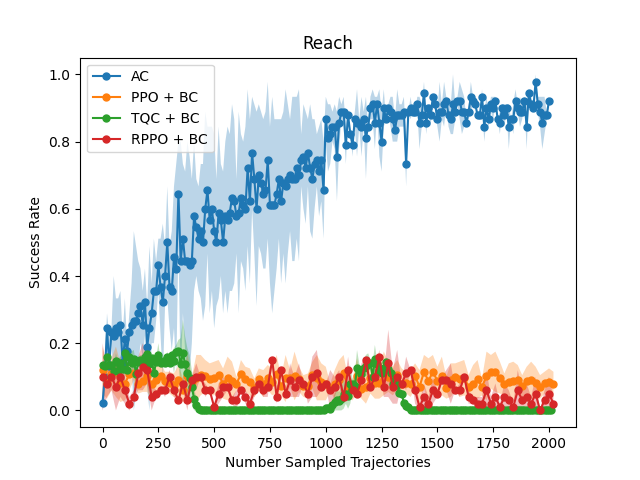
\includegraphics[width=\textwidth]{images/1_2000/Reach.png}
      \caption{1 expert demonstration.}
    \end{subfigure}
    \begin{subfigure}[t]{0.32\textwidth}
      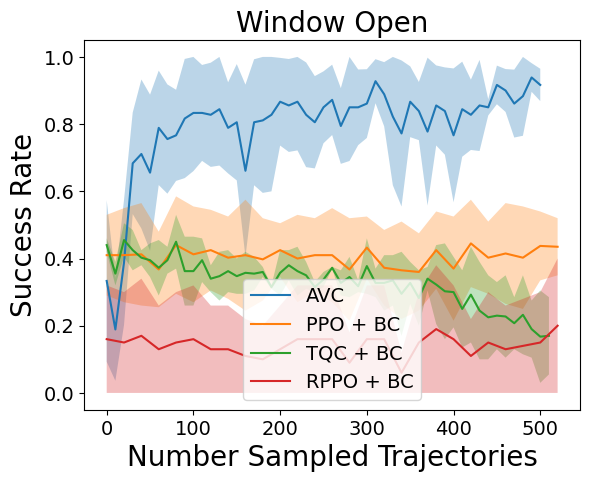
\includegraphics[width=\textwidth]{images/1_2000/Window Open.png}
      \caption{1 expert demonstration.}
    \end{subfigure}
    \begin{subfigure}[t]{0.32\textwidth}
      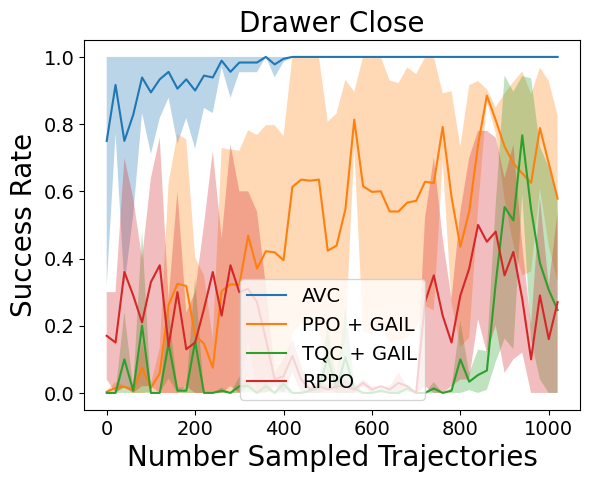
\includegraphics[width=\textwidth]{images/0/Drawer Close.png}
      \caption{0 expert demonstrations.}
      \label{fig:drawerclose}
    \end{subfigure}
    \medskip
    \begin{subfigure}[t]{0.45\textwidth}
      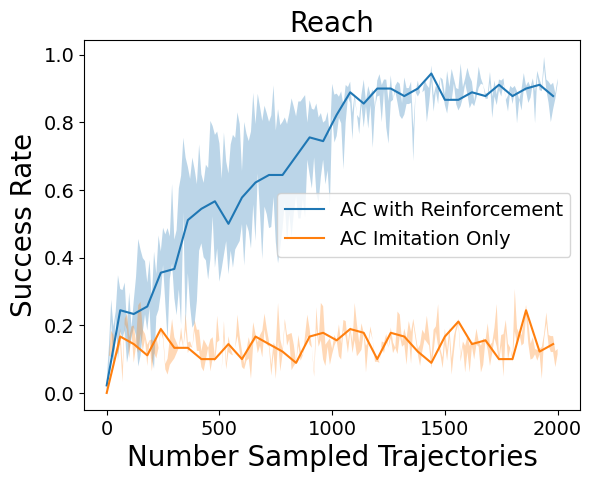
\includegraphics[width=\textwidth]{images/1_2000_imi/Reach.png}
      \caption{Reach environment. Comparison between pure imitation learning and reinforcement learning.}
    \end{subfigure}
    \hfill
    \begin{subfigure}[t]{0.45\textwidth}
      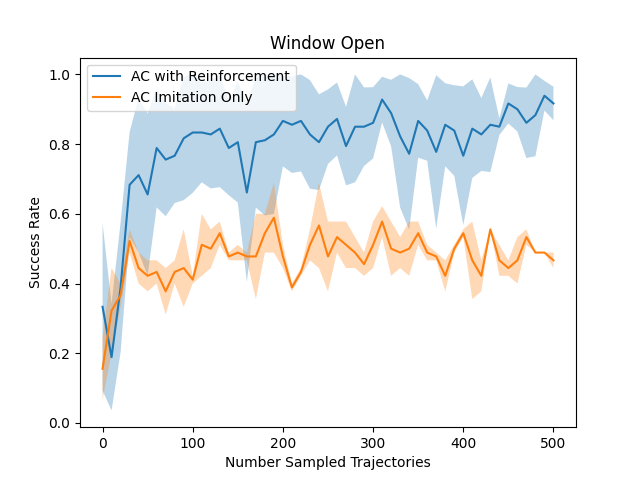
\includegraphics[width=\textwidth]{images/1_2000_imi/Window Open.png}
      \caption{Window Open environment. Comparison between pure imitation learning and reinforcement learning.}
    \end{subfigure}
    \caption{
    The learner trained by PPO, RPPO and TQC were pretrained using behavioural cloning given one demonstration except in the drawer close environment. 
    The pure imitation learning experiments on the buttom row were conducted using no additional episodes from the environment. There, the x-axis 
    displays equal amount of compute compared to the reinforcement learning runs.
    Each experiment was repeatet three times with 
    50 sampled validation episodes per run and data point. The shaded region displays one standard deviation.}
    \label{fig:guided_ref}
\end{figure}

The AVC algorithm was able to solve all environments with high success rates after 1000 or 2000 sampled trajectories. In "Reach" and "Window Open" the initial performance
of behavioural cloning was not improved in the reinforcement phase by any of the baselines. Similar to our discussion in section \ref{sec:fine_tuning},
we had to choose small learning rates to prevent catastrophic forgetting. With higher learning rates, all algorithms dropped to $0 \%$ success rate and did
not recover in initial tests. We find from the experiments that the challenging one observation sparse reward environment is difficult to learn in for
traditional actor critic algorithms. In these setups, AVC shows a significant improvement.\\

___________________________subsubsection --expert demonstratinos
First we wanted to rule out that the performance difference comes mainly from our behavioural cloning setup. As PPO and TQC natively don't make use of expert demonstrations,
we pretrained them using behavioural cloning. We expected that from the pretraining, at least one successful trajectory would be sampled in the training phase, thus
helping to overcome the initial search problem. We find that all algorithms perform significantly above $0\%$ success rate, so we conclude that all algorithms had
access to guidance to find successful trajectories. To further rule out that our methodology gives an unequal advantage to our algorithm, we tested all algorithms with 
zero expert demonstrations on the 
"Drawer Close" environment. We find that random trajectories can already solve the environment with about $20\%$ success rate, so no expert guidance is needed to learn a feasible behaviour.
The results are shown in subfigure \ref{fig:drawerclose}.\\ 

Notable, AVC performs significantly better then the baselines at the first datapoint of the plot. This is unexpected, since it indicates 
random behaviour from randomly initialisation of the policies. In further tests, we found that the initial success rate is either close to one or close to zero for all policies. This is likely 
due to the fact, that the initial observations for the "Drawer Close" environment are close in $L_2$ distance, thus a random policy will act similar in all environments. We find if that behaviour 
solves one enviroment, it solves all with high probability. In the three runs of the experiment, AVC was randomly initialized to have a high success rate in two runs, while PPO and TQC had no 
initial success. We did not have time to repeat the experiment until the initial performance of the algorithms converge. However, in train mode, 
all algorithms sample trajectories randomly in the initial training phase. 
We set the initial random phase to 1000 steps or 10 trajectories, so all algorithms had access to some successful trajectories with high probability. While the initialisation was an advantage 
for our algorithm in these experiment runs, it can still clearly be seen, that our algorithm is more stable and small variance in its performance compared to the baselines. In a later 
section, we also conduct an experiment on the "Drawer Close" enviroment with continued observations, as seen in figure \ref{fig:dense_ref}. We will discuss the figure in more detail later, but 
notice, that in the runs AVC started from $0 \%$ success rate and managed to find a good policy quickly, which we take as further evidence that the results of the "Drawer Close" experiment were not 
mainly due to luck. The overall high variance in the runs shown from the baselines can be explained by the sparse rewards, which provide highly non-linear feedback. 
AVC rapidly improved to perfect performance within about 400 steps. \\

___________________________subsubsection - NN achitecture
Next, we wanted to rule out that the observed performance gain of AVC over the baselines in the environments with expert demonstrations comes mostly from increased perforamce in imitation learning 
from the different underlying neural network architectures. AVC uses transformer encoders for the actor and 
critic, while the TQC and PPO implementations use MLPs and the RPPO implementation uses a GRU.\\ 
We tested the performance of AVC using pure imitation learning shown on the bottom row of
figure \ref{fig:guided_ref}. We find AVC significantly benifits from the reinfocement phase over pure imitation learning. \\
Overall, we take these finding as evidence for the effectiveness of the reinfocement aspect of the AVC algorithm.

\subsection{Comparison of Optimisation Modes}
\label{ref:com_opt_modes}
In section \ref{sec:inf_time_search} we discussed that we can use different modes of optimisation during inference time to optimize the action sequemce. In this section, 
we showcase the difference between optimising the action sequence directly and optimising the actor and planner weights. We tested the two different 
modes in the reach environment with the same setup as in section \ref{sec:g_ref_ler}, thus we used the same data for the actor planner optimisation runs. For the direct 
action optimisation runs we used 20000 sampled episodes to see, if reinforcement learning took place at all, as for the first 2000 episodes no improvement above 
imitation learning performance is seen. For this reason, we only repeated the experiment twice, as it took a long time to compute. The results are depicted in figure 
\ref{fig:action_vs_actor}. It is obvious, that the optimisation mode is key to the reinforcement learning performance. \\

In the bottom row of Figure \ref{fig:action_vs_actor}, the original generated trajectories (green) for the four action dimensions 
are shown alongside the optimized trajectories (orange) obtained using the gradient from the critic. We call the optimisation mode 
where we apply the gradient directly to the actions "action optimisation mode" and the optimisation mode where we apply 
the gradient to the actor and planner networks and recalculate the trajectories given the changed networks "actor planner 
optimisation mode".\\

We hypothesise that 
the actor planner optimisation mode's much faster convergence rate is due to the actor and planner networks ability to 
encode an informed representation of the useful trajectory space. This informed representation guides the gradient search 
given by the critic, leading to more efficient exploration. Subfigure \ref{fig:direct_actions} illustrates the trajectory 
changes resulting from the action optimisation mode, while Subfigure \ref{fig:ac_pl_actions} displays 
the trajectory changes resulting from the actor planner optimisation mode. \\

We observe that the actor planner 
optimisation mode produces a structured search, whereas the direct action optimisation mode's trajectory changes are less structured.\\

\begin{figure}[htbp]
    \centering
    \begin{subfigure}[t]{0.65\textwidth}
      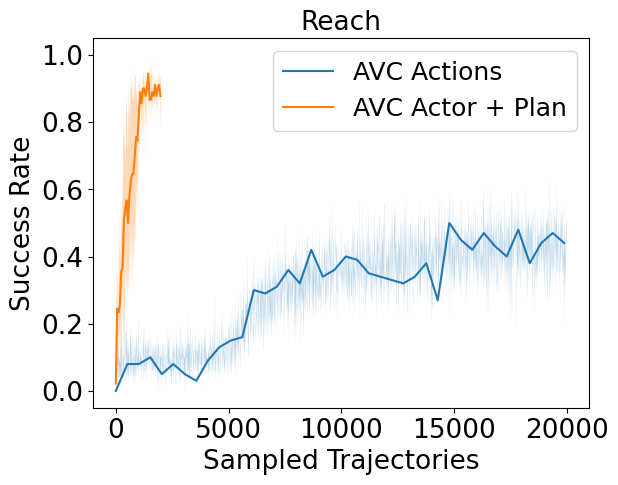
\includegraphics[width=\textwidth]{images/Plan_vs_Actions/Reach.png}
      \caption{Reach environment. Shown is the difference in learning efficiency of the active critic algorithm using two different optimisation modes.}
      \label{fig:plot1}
    \end{subfigure}
    \medskip
    \begin{subfigure}[t]{0.45\textwidth}
      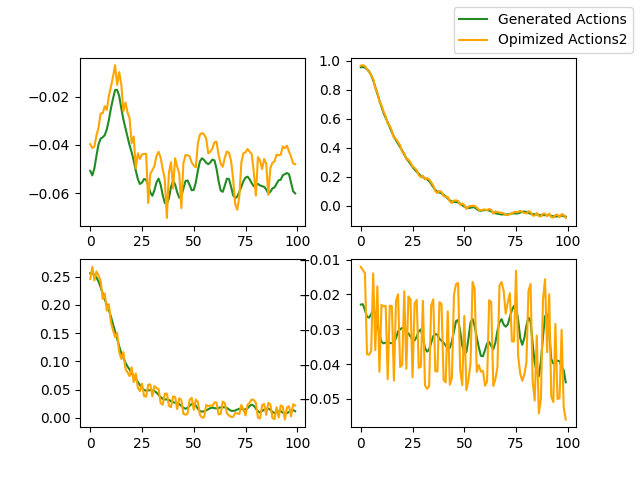
\includegraphics[width=\textwidth]{images/Plan_vs_Actions/changes/actions_1.png}
      \caption{Optimized trajectories (orange) and trajectories generated by the actor (green). The gradient from the critic was applied to the actions.}
      \label{fig:direct_actions}
    \end{subfigure}
    \hfill
    \begin{subfigure}[t]{0.45\textwidth}
      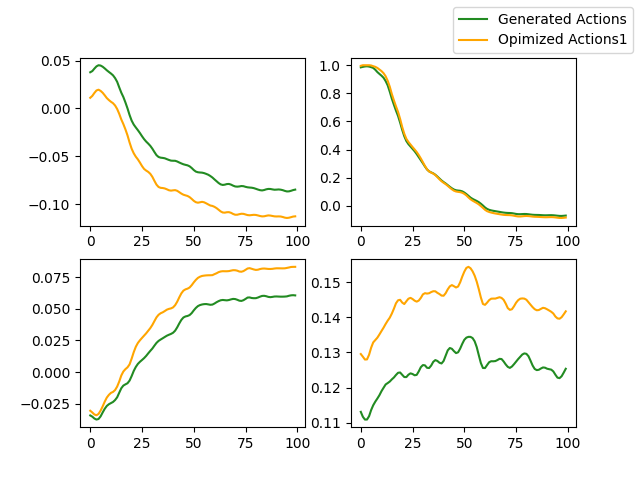
\includegraphics[width=\textwidth]{images/Plan_vs_Actions/changes/plans_actor_0.png}
      \caption{Optimized trajectories (orange) and trajectories generated by the actor (green). The gradient from the critic was applied to the actor and planner.}
      \label{fig:ac_pl_actions}
    \end{subfigure}
    \caption{Comparison of two different optimisation modi. The experiments have four action dimensions, which are depicted in the 
    four plots per figure on the buttom row.}
    \label{fig:action_vs_actor}
\end{figure}

\subsection{Dense Observations}
In this section we test the relaxation of the AVC algorithm to MDP environments, developed in section \ref{sec:relax_dense}, with the environment state given as an observation after each step. \\
We use sparse rewards 
and compare continued observation active critic (DOAVC) to PPO and TQC on the "Reach", "Window Open" and "Drawer Close" environments. Again, we don't use "HER", as it limits the generality of 
the approach. Apart from 
providing an observation per time step,
we use the same setup as described in previous sections. The results are shown in figure \ref{fig:dense_ref} for three runs per experiment.\\ 

First, we note that both baseline algorithms exhibit similar performance in behavioural cloning as in the single 
observation setup. This is unsurprising as behavioural cloning does not rely on interactions with the environment. \\

After the first data point, both algorithms sharply drop to near zero success rate, which displays that catastrophic forgetting is more 
pronounced than in the single observation enviroment. We explain this with the distribution shift after training starts. A policy trained by imitation learning 
will induce a different distribution of observations then the expert data. This breaks the i.i.d. assumption. In the single observation case for PPO and TQC, this assumption was not broken, 
since the inputs for the whole trajectory are computed from the first observation. The distribution of the first observations is a constant of the enviroment.\\

PPO did not find solutions to the "Reach" and "Window Open" environments, 
but we find TQC got about $20 \%$ success rate on "Reach" and achieved about $80 \%$ success rate on "Window Open" leveling out after about 2500 episodes. 
The superior performance of TQC over PPO is expected, as TQC tends to perform better in environments where exploration is important. As TQC now gets 
feedback from it's actions on the environment, the better exploration is an advantage over PPO.\\ 

In particular, as TQCs performance drops to about $0 \%$ for the "Window Open" 
environment after the first data point, we wanted to analyze, if TQC uses the guidance from the expert at all, or if it starts from 
no usable knowledge about the environment. To do this, we also conducted the experiment three times with no initial behavioural cloning. The results are shown in 
subfigure \ref{fig:TQC_0_vs_exp}. We observe that TQC can solve the environment within 5000 steps from no expert demonstrations in one case, but does not find a good policy in the other two. 
We propose pretraining from behavioural cloning is a useful bias for the algorithm to find feasable solutions quicker with higher probability.\\ 

Following this insight, 
we also conducted the "Window Open" experiment in MDP setting with GAIL to make better use of the provided expert demonstration. We find our initial 
baseline with pretrained TQC performs best. This is probably due to the fact that GAIL makes no use of the sparse reward. Additionaly, 
the authors mentioned in the paper, that GAIL is not more efficient in terms of environment interactions then TRPO with rewards. A large number of 
environment interactions are needed, before the discriminator of GAIL provides useful rewards for the learner. We suppose that is a reason, why GAIL does not perform 
well in our setting, where relatively small amount of environment interactions are used. \\

We also included results for the "Drawer Close" environment with no expert demonstrations. All algorithms perform better than in the single observation environment, 
but DOAVC is the only algorithm with stable performance. It found a solution with near perfect success rate in all three runs quickly. \\

Overall, DOAVC performs well in all shown environments. Especially in the "Reach" environment it is the only algorithm that finds a feasable solution while it 
converges much quicker and has a more robust bahaviour in general. 




\begin{figure}[htbp]
  \centering
  \begin{subfigure}[t]{0.45\textwidth}
    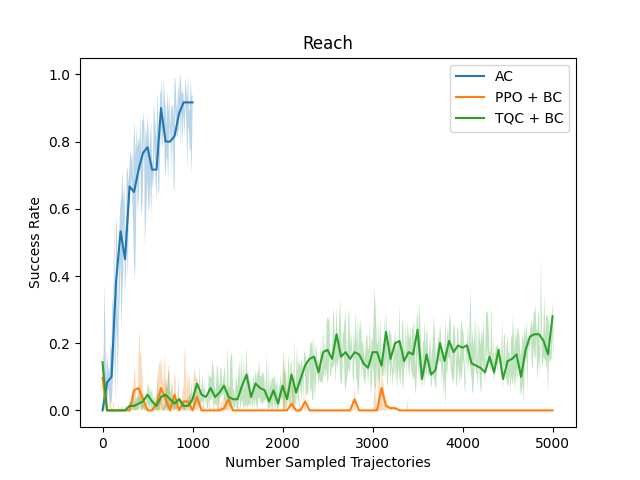
\includegraphics[width=\textwidth]{images/dense_1/Reach.png}
    \caption{One expert demonstration.}
  \end{subfigure}
  \hfill
  \begin{subfigure}[t]{0.45\textwidth}
    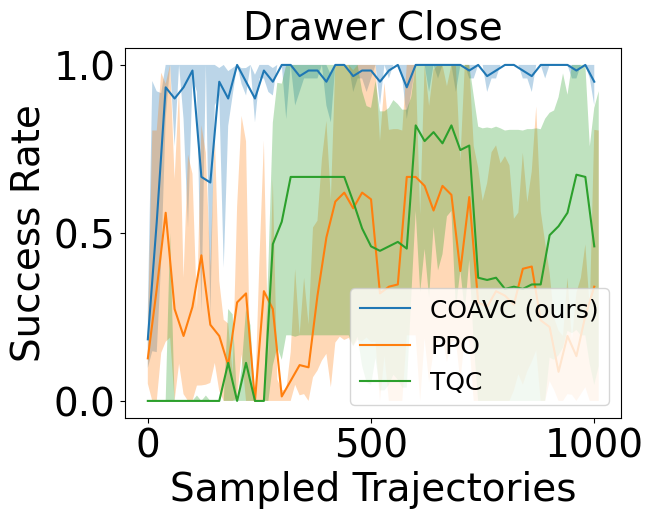
\includegraphics[width=\textwidth]{images/dense_0/Drawer Close.png}
    \caption{No expert demonstrations.}
  \end{subfigure}
  \medskip
  \begin{subfigure}[t]{0.45\textwidth}
    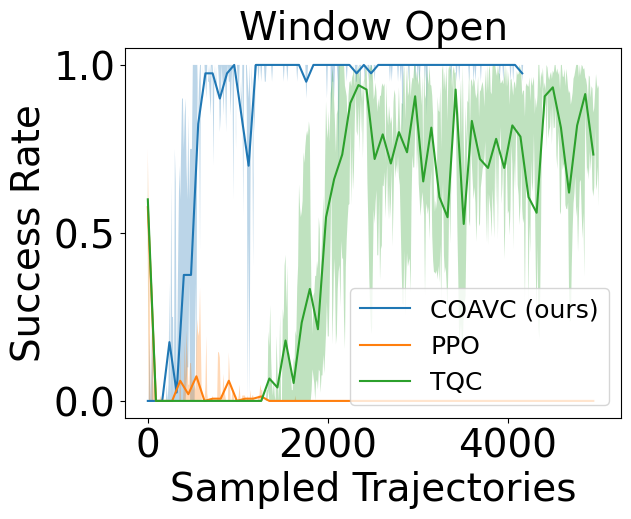
\includegraphics[width=\textwidth]{images/dense_1/Window Open.png}
    \caption{One expert demonstration.}
  \end{subfigure}
  \hfill
  \begin{subfigure}[t]{0.45\textwidth}
    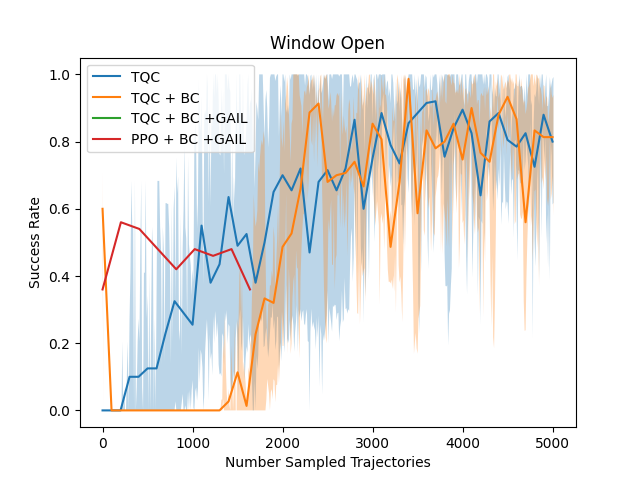
\includegraphics[width=\textwidth]{images/TQC_bc_GAIL_vs_ref/Window Open.png}
    \caption{Comparison between TQC with no expert demonstrations and expert guided baselines.}
    \label{fig:TQC_0_vs_exp}
  \end{subfigure}
  \caption{Comparison between DOAVC and various baselines given one or no expert demonstrations. The environment state was provided after each step.
  Each experiment was repeated three times with 50 evaluation episodes per data point.}
  \label{fig:dense_ref}
\end{figure}

\subsection{Comparison of Continued and Single Observation}
In this section we compare DOAVC and AVC, to investigate if DOAVC makes use of the additionally provided information from the continued observations. 
The results are shown in figure \ref{fig:dense_vs_single}.\\

We observe that in "Reach" and "Drawer Close", DOAVC converges quicker. Especially in "Reach", we see a stable improvement from DOAVC over AC. In "Drawer Close", the difference is 
small, which is mainly due to the fact that AVC already solves the environment very quickly. Note however, that DOAVC had worse initial performance then AVC in the shown experiments. 
As previously discussed, the initial performance is determined by random initialisation of the networks and can exhibit substantial 
variance.\\ 

The observation that DOAVC achieved convergence at a faster rate than AVC, despite starting with inferior initializations in 
all three runs, provides additional support for the proposition that DOAVC makes effective use of the continued observations. \\

In the "Window Open" environment, DOAVC initially converged slower but 
reached near perfect performance quicker then AC. We suppose this is due to the different optimisation modes used for the two algorithms. Recall that AVC optimizes the whole 
trajectory at the beginning, while DOAVC makes small improvements per time step, due to self imposed inference time constraints. We expect this has the effect that in inference time, the critic of 
AVC can make larger changes to the trajectory proposed by the actor. In other words, DOAVC makes smaller moves towards the critic target than AC. Also out of time constraints, we could 
not conduct a hyperparameter search for DOAVC. It is possible that DOAVC would converge quicker, given more optimisation steps per inference step or a higher inference optimisation 
learning rate $\alpha_{inf}$.\\ 

AVC already performs close to the MDP setup used by DOAVC. We propose this is due to the fact, that AVC uses the information about the environment 
from the expert demonstrations effectively to search for new candidate solutions. As discussed in section \ref{ref:com_opt_modes}, AVC searches on a prestructured subspace given the "knowledge" of the 
actor. This means it does not conduct random search even though it does not get any feedback from the environment. This is probably a key for the good performance of AVC and DOAVC and explains 
the relative close performance of both algorithms. We expect a major advantage of DOAVC over AVC in non-deterministic environments, as AVC will not be able to solve those from the initial 
observation alone. DOAVC already has a method to disambiguate action sequences given the same observations as discussed in section \ref{avr_action_problem}. This is key, if the same initial 
observations and actions can lead to different observations at later time steps. However out of time constraints, we leave this research question to future work.\\
Overall, we find that DOAVC works well in the tested environments and outperforms all baselines in the MDP setting with sparse rewards.

\begin{figure}[htbp]
  \centering
  \begin{subfigure}[t]{0.32\textwidth}
    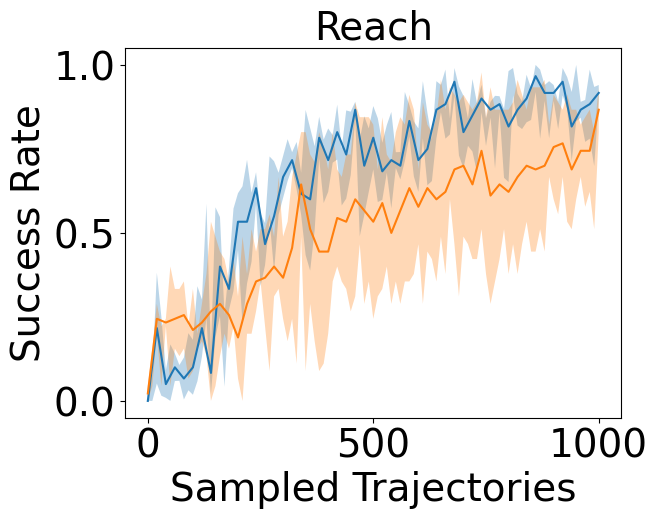
\includegraphics[width=\textwidth]{images/dense_vs_sparse_1/Reach.png}
    \caption{1 expert demonstration.}
  \end{subfigure}
  \medskip
  \begin{subfigure}[t]{0.32\textwidth}
    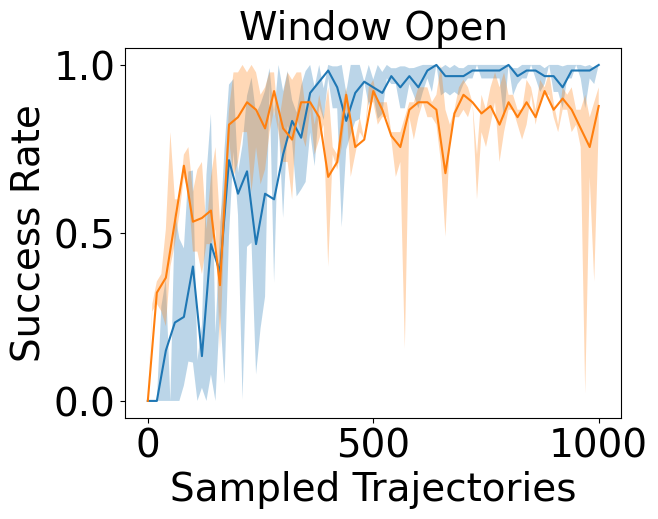
\includegraphics[width=\textwidth]{images/dense_vs_sparse_1/Window Open.png}
    \caption{1 expert demonstration.}
  \end{subfigure}
  \hfill
  \begin{subfigure}[t]{0.32\textwidth}
    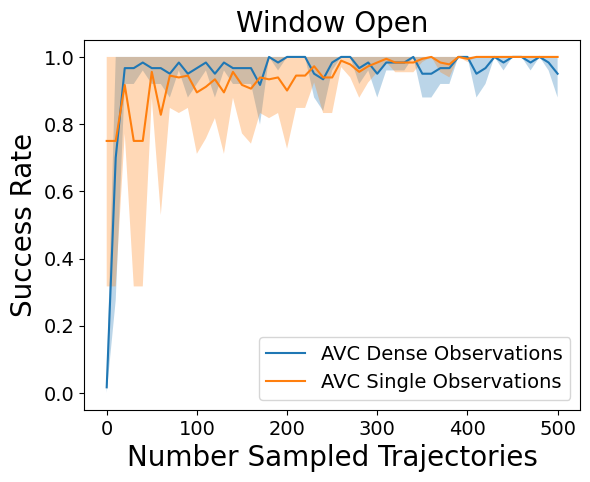
\includegraphics[width=\textwidth]{images/dense_vs_sparse_0/Window Open.png}
    \caption{0 expert demonstrations.}
  \end{subfigure}
  \caption{Comparison of AVC in single observation and DOAVC in continued observation MDP environments. Each experiment was repeated three times with 30 evaluation episodes per data point.
  }
  \label{fig:dense_vs_single}
\end{figure}

% !TEX root = ../main.tex

\chapter{Discussion}
\label{chapter:Discussion}
In this chapter we will summarize our findings and discuss advantages as well es remaining limitations of our approach and evaluation.
\section{Applicability and Advantages}
\subsection{Imitation Learning}
Our results from section \ref{sec:exp_imi_lr} demonstrate that our imitation learning approach outperforms recurrent algorithms in continuous action space, 
given a single observation per trajectory. We propose this is due to generating the whole sequence in one step, 
rather than using an autoregressive approach. This method does not break the i.i.d. assumption, making predictions more robust and effective 
for planning in continuous space. \\

\subsection{Optimisation Mode}
In Section \ref{ref:com_opt_modes}, we conducted an analysis of various optimisation modes employed in the active critic algorithm. 
Our experiments revealed that the optimisation mode plays a critical role in determining the reinforcement learning performance. 
Specifically, we propose leveraging the actor to encode a useful space of candidate solutions that the critic can search on. 
This approach allows for informed search and leads to faster convergence and more efficient exploration of candidate solutions. We take the strong effect of the inference time 
search paradigm on the convergence rate of the algorithm as evidence for the importance and effectiveness of our use of inference time search.

\subsection{Reinforcement Learning}
We explored the effectiveness of reinforcement learning in improving the performance of our approach as compared to pure imitation learning. 
Our results in section \ref{sec:fine_tuning} demonstrate that our approach can effectively leverage both expert demonstrations and reinforcement learning data to achieve 
superior performance compared to our baselines.\\

To further assess the impact of reinforcement learning, we conducted experiments on the Drawer Close environment without expert demonstrations. 
In this environment, a solution can be achieved through random trajectories to some degree. 
Our analysis revealed that our algorithm outperformed the baselines significantly in this pure reinforcement setting, 
indicating that our approach is more stable with sparse rewards than traditional actor critic methods.\\




\subsection{MDP Setting}
In Section \ref{sec_exp_con_obs}, we evaluated the performance of the continued observation active critic (COAVC) approach in the standard MDP setting, 
where observations are available after each step.\\

Our experiments demonstrated that our method significantly outperforms the baselines, making efficient use of expert demonstrations and reinforcement learning.\\

To evaluate the performance of pure reinforcement learning in MDPs, we conducted experiments on the Drawer Close 
environments without expert demonstrations. Our results show that all baselines and COAVC can find solutions, but COAVC is more stable and achieves 
faster convergence. These findings provide further evidence of the general applicability and better performance of our approach over the baselines. 

\subsection{Single Observation and MDP Comparison}
We compared COAVC to AVC in section \ref{sec:com_coavc_avc} and observed that while COAVC performs better, 
AVC already achieves high accuracy in solving environments. We attribute this to the structured exploration enabled by knowledge from 
expert data. Moreover, the inference of AVC is i.i.d., while that of COAVC is not, as observations at inference time are dependent on actions. 

In conclusion, our experiments demonstrate that the AVC paradigm is highly stable and performs well in settings with sparse rewards. 
It effectively leverages expert demonstrations for both exploitation and informed search. While COAVC provides improved performance over 
AVC, the latter already achieves high accuracy in solving environments.

\section{Limitations and Drawbacks}
\subsection{Baselines}
We have chosen general-purpose reinforcement learning algorithms for our baselines, because our paradigm is also generally applicable 
and we wanted to test it in a wide range of experiments, including those with no expert demonstrations.\\ 

However, we think it is interesting to test the specific strength in finetuning against baselines which are 
tailored for it. In section Guided Reinforcement Learning with Sparse Rewards \ref{sec:rel_work_finetuning} of our related work, we introduced 
a candidate. While we argued why we expect our algorithm to perform better in cases with provided expert demonstrations than the featured algorithm, we have to 
leave testing it for future work.\\

Another aspect that we would like to test in more depths is the sparse reward setting. In section \ref{sec:HER}, we have introduced two concepts that are used for sparse reinforcement learning, namely 
HER and curiosity driven exploration. While HER is not generally applicable, we would like to both test our approach against a baseline using curiosity, as well as incorporate 
curiosity into our algorithm as an additional reward signal. 

\subsection{Exploration}
Although COAVC outperformed baselines, its performance in the Pick and Place and Push environments did not reach near-perfect levels, 
indicating limitations in more challenging environments. While a longer reinforcement phase might improve performance, this was not explored 
due to time constraints. AVC currently does not use a stochastic actor, which we expect to be key for improved exploration.\\ 

Additionally, exploration from no expert demonstrations was not extensively studied, except for the Drawer Close 
environment. We expected pure reinforcement learning is not feasible for more challenging environments given sparse rewards. 
However, we found TQC was able to solve the Window Open environment without expert demonstrations, but further investigation on whether 
COAVC performs well in this environment was not possible due to time constraints.\\ 

  

\subsection{Indeterminacy}
In COAVC, the critic estimates the expected reward given an action sequence and chooses the best sequence greedily. 
However, choosing the action sequence with the highest expected reward is not equivalent to choosing the action with the highest posterior 
expectation over both the environment dynamics and action sequences. In indeterministic environments, the optimal action sequence may depend on later observations. To 
search for the best current action in an indeterministic MDP requires the estimate of multiple possible observations and action sequences, respectively. \\

In the current version, planning with multiple possible action sequences that can depend on later observations is not possible. 
Although COAVC can update the action sequence given new observations, it can not plan for multiple possible future observations.

% !TEX root = ../main.tex

\chapter{Conclusion & Future Work}
\label{chapter:Conc_Fut}
In this thesis, we have presented the \ac{avc} paradigm, which effectively employs search on continuous action spaces and utilizes 
expert demonstrations to solve sparse reward \ac{rl} tasks. Our results demonstrate that \ac{avc} 
outperforms state-of-the-art general-purpose \ac{rl} algorithms in a variety of robot manipulation tasks, achieving superior performance 
while maintaining high sample efficiency. We provided evidence that search is a critical component that enables us to make the best use of available 
environment interactions.

\section{Future Work}
\subsection{Indeterminacy}
Our current search paradigm does not account for the various possible future observations, which poses a significant challenge in 
continuous observation and action spaces where enumeration is impossible. To address this issue, we propose incorporating a stochastic 
representation of observations to sample from a probability density estimate provided by the critic. 
This approach could prove promising in developing an efficient search paradigm in such environments.

\subsection{Uncertainty Estimate}
Modelling an uncertainty estimate could be another crucial aspect of improving our search paradigm. 
Currently, the critic searches for solutions with a high expected probability without considering uncertainty. 
Incorporating an uncertainty estimate could assist the critic in finding solutions that maximize expected reward with high confidence. 
Existing uncertainty-aware approaches \cite{gawlikowski2022survey,liu2022simple} 
could be integrated into the \ac{avc} algorithm.

\subsection{Curiosity Driven Exploration}
To further enhance exploration, we could incorporate curiosity-driven exploration approaches \cite{pathak2017curiositydriven}. 
Curiosity provides an intrinsic reward that could be specifically useful in sparse reward settings. 
Currently, the \ac{avc} algorithm selects a provided trajectory if the critic estimates that it solves the environment. By incorporating curiosity, 
we can explore more robust solutions or gain a better understanding of \ac{mdp} dynamics by modifying trajectories even in environments that the 
algorithm can already solve. Here, incorporating an uncertainty estimate could be beneficial as well.



% ---------------------------------------------------------------------------
%
% Appendix
%
% ---------------------------------------------------------------------------
\part*{Appendix}
\addcontentsline{toc}{part}{Appendix}

\appendix %---------------------------------------

% !TEX root = ../main.tex
\chapter{Implementation Details}
%\section{Detailed Validation Results}
\label{chapter:DetailedDescriptions}\label{appendix}
%\inputminted{c++}{../../src/wos_native.cuh}

\chapter{Meta World}
\label{chapter:MetaWorld}\label{appendix}

\chapter{Additional Plots}

\begin{figure}[htbp]
    \centering
    \begin{subfigure}[b]{0.45\textwidth}
      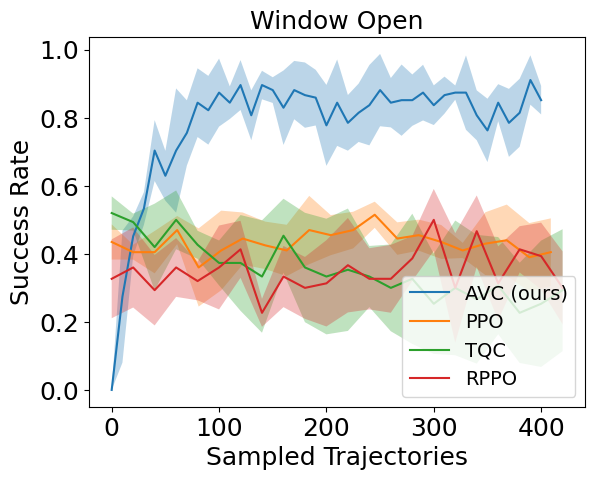
\includegraphics[width=\textwidth]{images/4_400/Window Open.png}
      \caption{Window Open environment.}
      \label{fig:plot1}
    \end{subfigure}
    \hfill
    \begin{subfigure}[b]{0.45\textwidth}
      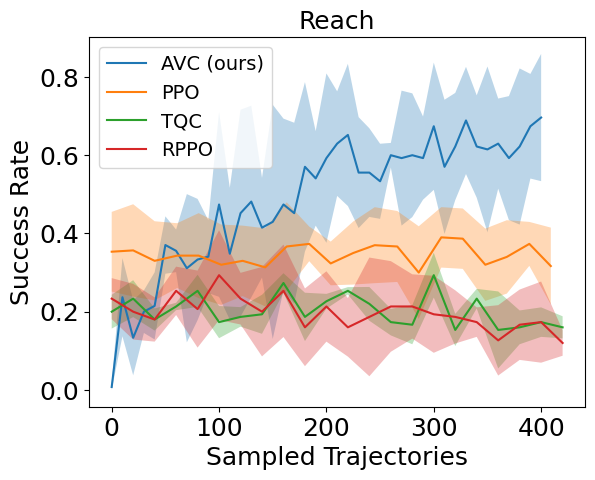
\includegraphics[width=\textwidth]{images/4_400/Reach.png}
      \caption{Reach environment.}
      \label{fig:plot2}
    \end{subfigure}
    \medskip
    \begin{subfigure}[b]{0.45\textwidth}
      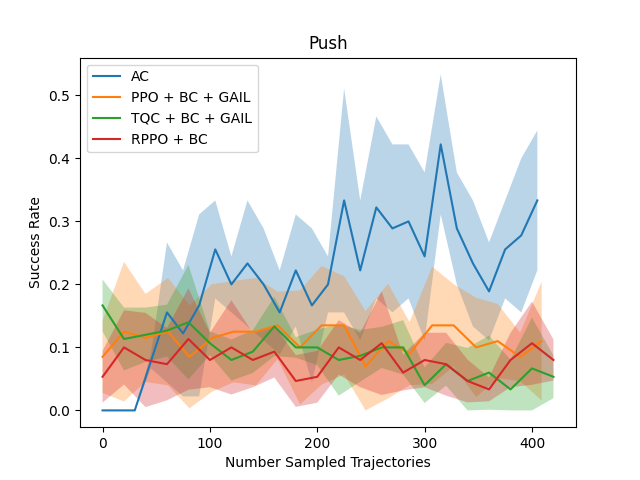
\includegraphics[width=\textwidth]{images/4_400/Push.png}
      \caption{Push environment.}
      \label{fig:plot3}
    \end{subfigure}
    \hfill
    \begin{subfigure}[b]{0.45\textwidth}
      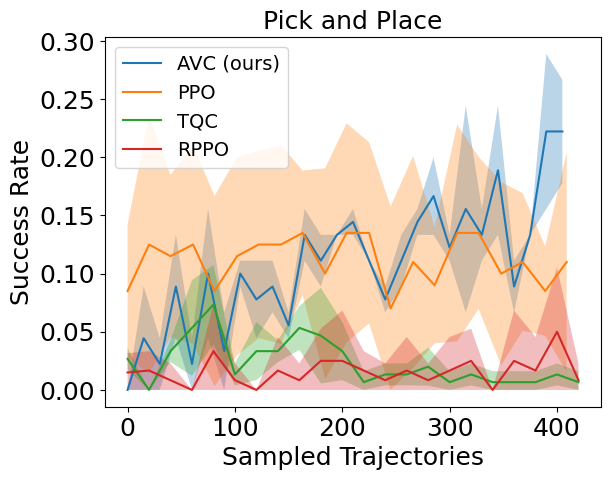
\includegraphics[width=\textwidth]{images/4_400/Pick and Place.png}
      \caption{Pick and Place environment.}
      \label{fig:plot4}
    \end{subfigure}
    \caption{Each learner had access to 4 expert demonstrations. 
    The learner trained by GAIL and RPPO were pretrained using behavioural cloning given the 4 demonstrations. 
    The x-axis shows the number of sampled environment epsiodes, each with 100 steps. One initial observation and a sparse reward signal at the end of each episode was provided.}
    \label{fig:4}
\end{figure}

\begin{figure}[htbp]
    \centering
    \begin{subfigure}[b]{0.45\textwidth}
      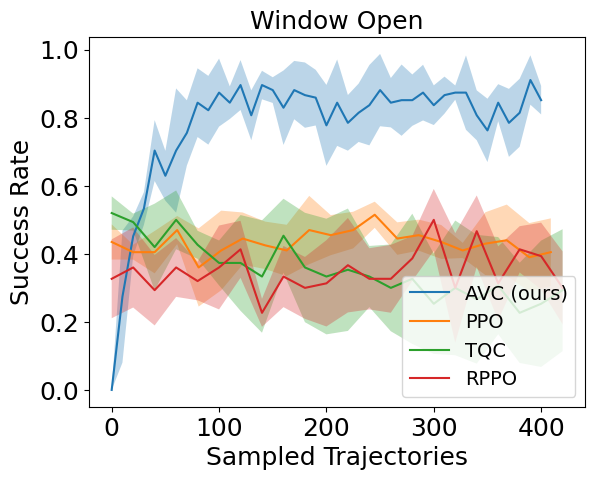
\includegraphics[width=\textwidth]{images/4_400/Window Open.png}
      \caption{Window Open environment.}
      \label{fig:plot1}
    \end{subfigure}
    \hfill
    \begin{subfigure}[b]{0.45\textwidth}
      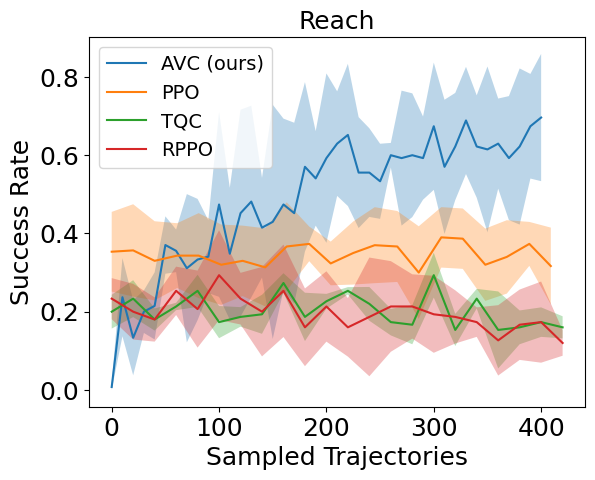
\includegraphics[width=\textwidth]{images/4_400/Reach.png}
      \caption{Reach environment.}
      \label{fig:plot2}
    \end{subfigure}
    \medskip
    \begin{subfigure}[b]{0.45\textwidth}
      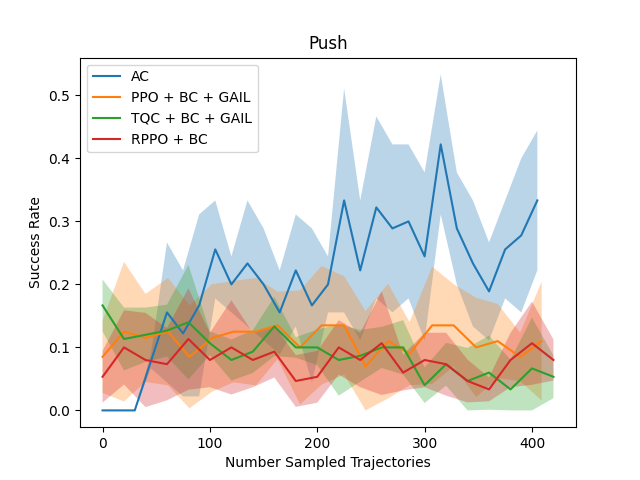
\includegraphics[width=\textwidth]{images/4_400/Push.png}
      \caption{Push environment.}
      \label{fig:plot3}
    \end{subfigure}
    \hfill
    \begin{subfigure}[b]{0.45\textwidth}
      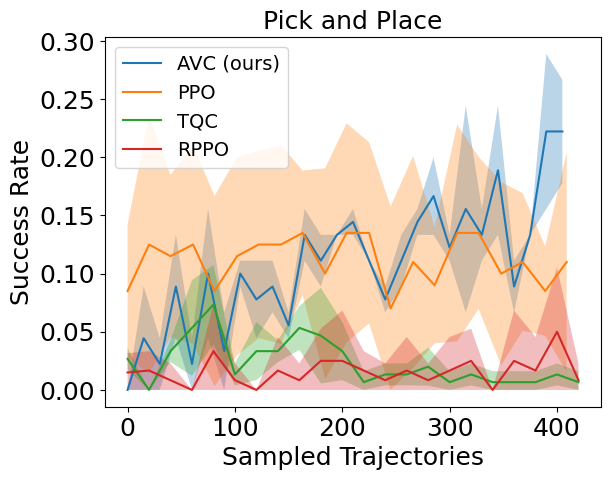
\includegraphics[width=\textwidth]{images/4_400/Pick and Place.png}
      \caption{Pick and Place environment.}
      \label{fig:plot4}
    \end{subfigure}
    \caption{Each learner had access to 4 expert demonstrations. 
    The learner trained by GAIL and RPPO were pretrained using behavioural cloning given the 4 demonstrations. 
    The x-axis shows the number of sampled environment epsiodes, each with 100 steps. One initial observation and a sparse reward signal at the end of each episode was provided.}
    \label{fig:4}
\end{figure}


 \clearemptydoublepage

 \printglossaries

 \addcontentsline{toc}{chapter}{Bibliography}
 \printbibliography
\end{document}
